% Options for packages loaded elsewhere
\PassOptionsToPackage{unicode}{hyperref}
\PassOptionsToPackage{hyphens}{url}
%
\documentclass[
]{book}
\usepackage{amsmath,amssymb}
\usepackage{iftex}
\ifPDFTeX
  \usepackage[T1]{fontenc}
  \usepackage[utf8]{inputenc}
  \usepackage{textcomp} % provide euro and other symbols
\else % if luatex or xetex
  \usepackage{unicode-math} % this also loads fontspec
  \defaultfontfeatures{Scale=MatchLowercase}
  \defaultfontfeatures[\rmfamily]{Ligatures=TeX,Scale=1}
\fi
\usepackage{lmodern}
\ifPDFTeX\else
  % xetex/luatex font selection
\fi
% Use upquote if available, for straight quotes in verbatim environments
\IfFileExists{upquote.sty}{\usepackage{upquote}}{}
\IfFileExists{microtype.sty}{% use microtype if available
  \usepackage[]{microtype}
  \UseMicrotypeSet[protrusion]{basicmath} % disable protrusion for tt fonts
}{}
\makeatletter
\@ifundefined{KOMAClassName}{% if non-KOMA class
  \IfFileExists{parskip.sty}{%
    \usepackage{parskip}
  }{% else
    \setlength{\parindent}{0pt}
    \setlength{\parskip}{6pt plus 2pt minus 1pt}}
}{% if KOMA class
  \KOMAoptions{parskip=half}}
\makeatother
\usepackage{xcolor}
\usepackage{color}
\usepackage{fancyvrb}
\newcommand{\VerbBar}{|}
\newcommand{\VERB}{\Verb[commandchars=\\\{\}]}
\DefineVerbatimEnvironment{Highlighting}{Verbatim}{commandchars=\\\{\}}
% Add ',fontsize=\small' for more characters per line
\usepackage{framed}
\definecolor{shadecolor}{RGB}{248,248,248}
\newenvironment{Shaded}{\begin{snugshade}}{\end{snugshade}}
\newcommand{\AlertTok}[1]{\textcolor[rgb]{0.94,0.16,0.16}{#1}}
\newcommand{\AnnotationTok}[1]{\textcolor[rgb]{0.56,0.35,0.01}{\textbf{\textit{#1}}}}
\newcommand{\AttributeTok}[1]{\textcolor[rgb]{0.13,0.29,0.53}{#1}}
\newcommand{\BaseNTok}[1]{\textcolor[rgb]{0.00,0.00,0.81}{#1}}
\newcommand{\BuiltInTok}[1]{#1}
\newcommand{\CharTok}[1]{\textcolor[rgb]{0.31,0.60,0.02}{#1}}
\newcommand{\CommentTok}[1]{\textcolor[rgb]{0.56,0.35,0.01}{\textit{#1}}}
\newcommand{\CommentVarTok}[1]{\textcolor[rgb]{0.56,0.35,0.01}{\textbf{\textit{#1}}}}
\newcommand{\ConstantTok}[1]{\textcolor[rgb]{0.56,0.35,0.01}{#1}}
\newcommand{\ControlFlowTok}[1]{\textcolor[rgb]{0.13,0.29,0.53}{\textbf{#1}}}
\newcommand{\DataTypeTok}[1]{\textcolor[rgb]{0.13,0.29,0.53}{#1}}
\newcommand{\DecValTok}[1]{\textcolor[rgb]{0.00,0.00,0.81}{#1}}
\newcommand{\DocumentationTok}[1]{\textcolor[rgb]{0.56,0.35,0.01}{\textbf{\textit{#1}}}}
\newcommand{\ErrorTok}[1]{\textcolor[rgb]{0.64,0.00,0.00}{\textbf{#1}}}
\newcommand{\ExtensionTok}[1]{#1}
\newcommand{\FloatTok}[1]{\textcolor[rgb]{0.00,0.00,0.81}{#1}}
\newcommand{\FunctionTok}[1]{\textcolor[rgb]{0.13,0.29,0.53}{\textbf{#1}}}
\newcommand{\ImportTok}[1]{#1}
\newcommand{\InformationTok}[1]{\textcolor[rgb]{0.56,0.35,0.01}{\textbf{\textit{#1}}}}
\newcommand{\KeywordTok}[1]{\textcolor[rgb]{0.13,0.29,0.53}{\textbf{#1}}}
\newcommand{\NormalTok}[1]{#1}
\newcommand{\OperatorTok}[1]{\textcolor[rgb]{0.81,0.36,0.00}{\textbf{#1}}}
\newcommand{\OtherTok}[1]{\textcolor[rgb]{0.56,0.35,0.01}{#1}}
\newcommand{\PreprocessorTok}[1]{\textcolor[rgb]{0.56,0.35,0.01}{\textit{#1}}}
\newcommand{\RegionMarkerTok}[1]{#1}
\newcommand{\SpecialCharTok}[1]{\textcolor[rgb]{0.81,0.36,0.00}{\textbf{#1}}}
\newcommand{\SpecialStringTok}[1]{\textcolor[rgb]{0.31,0.60,0.02}{#1}}
\newcommand{\StringTok}[1]{\textcolor[rgb]{0.31,0.60,0.02}{#1}}
\newcommand{\VariableTok}[1]{\textcolor[rgb]{0.00,0.00,0.00}{#1}}
\newcommand{\VerbatimStringTok}[1]{\textcolor[rgb]{0.31,0.60,0.02}{#1}}
\newcommand{\WarningTok}[1]{\textcolor[rgb]{0.56,0.35,0.01}{\textbf{\textit{#1}}}}
\usepackage{longtable,booktabs,array}
\usepackage{calc} % for calculating minipage widths
% Correct order of tables after \paragraph or \subparagraph
\usepackage{etoolbox}
\makeatletter
\patchcmd\longtable{\par}{\if@noskipsec\mbox{}\fi\par}{}{}
\makeatother
% Allow footnotes in longtable head/foot
\IfFileExists{footnotehyper.sty}{\usepackage{footnotehyper}}{\usepackage{footnote}}
\makesavenoteenv{longtable}
\usepackage{graphicx}
\makeatletter
\def\maxwidth{\ifdim\Gin@nat@width>\linewidth\linewidth\else\Gin@nat@width\fi}
\def\maxheight{\ifdim\Gin@nat@height>\textheight\textheight\else\Gin@nat@height\fi}
\makeatother
% Scale images if necessary, so that they will not overflow the page
% margins by default, and it is still possible to overwrite the defaults
% using explicit options in \includegraphics[width, height, ...]{}
\setkeys{Gin}{width=\maxwidth,height=\maxheight,keepaspectratio}
% Set default figure placement to htbp
\makeatletter
\def\fps@figure{htbp}
\makeatother
\setlength{\emergencystretch}{3em} % prevent overfull lines
\providecommand{\tightlist}{%
  \setlength{\itemsep}{0pt}\setlength{\parskip}{0pt}}
\setcounter{secnumdepth}{5}
\usepackage{booktabs}
\usepackage{lscape}

\ifLuaTeX
  \usepackage{selnolig}  % disable illegal ligatures
\fi
\usepackage[]{natbib}
\bibliographystyle{apalike}
\IfFileExists{bookmark.sty}{\usepackage{bookmark}}{\usepackage{hyperref}}
\IfFileExists{xurl.sty}{\usepackage{xurl}}{} % add URL line breaks if available
\urlstyle{same}
\hypersetup{
  pdftitle={Basis Data dan Penelusuran Data},
  pdfauthor={Bakti Siregar, M.Sc},
  hidelinks,
  pdfcreator={LaTeX via pandoc}}

\title{Basis Data dan Penelusuran Data}
\author{Bakti Siregar, M.Sc}
\date{2023-08-26}

\begin{document}
\maketitle

{
\setcounter{tocdepth}{1}
\tableofcontents
}
\hypertarget{kata-pengantar}{%
\chapter*{Kata Pengantar}\label{kata-pengantar}}
\addcontentsline{toc}{chapter}{Kata Pengantar}

Selamat datang dalam modul praktikum mengenai basis data dan penelusuran data. Dalam era digital yang semakin maju, pengelolaan informasi dan akses terhadap data sangatlah penting. Basis data merupakan fondasi utama dalam pengelolaan data yang efisien dan terstruktur, sedangkan penelusuran data memungkinkan kita untuk menggali wawasan berharga dari kumpulan informasi yang tersedia. Dalam modul ini, kita akan menjelajahi konsep-konsep dasar dalam basis data, termasuk jenis-jenis basis data, model data, bahasa kueri, dan praktik terbaik dalam merancang basis data yang optimal. Secara khusus, mudul ini

Selain itu, penelusuran basis data yang menjadi fokus penting adalah menggunakan R Programing dan SQL dalam membuat data analytics system. Penelusuran data melibatkan teknik-teknik dan alat-alat untuk menggali informasi yang berharga dari kumpulan data yang besar dan kompleks. Dengan adanya kemajuan dalam analisis data dan kecerdasan buatan, penelusuran data telah menjadi aspek penting dalam pengambilan keputusan dan inovasi. Penulis berharap bimbingan ini akan memberikan pemahaman yang kokoh tentang basis data dan penelusuran data, serta memberi Anda wawasan yang berguna dalam mengelola data dan mengambil informasi berharga dari sumber daya yang ada. Selamat belajar!

\hypertarget{ringkasan-materi}{%
\section*{Ringkasan Materi}\label{ringkasan-materi}}
\addcontentsline{toc}{section}{Ringkasan Materi}

Adapun isi pembelajaran dalam modul ini adalah sebagai berikut:

\begin{itemize}
\tightlist
\item
  Bab 1
\item
  Bab 2
\item
  Bab 3
\item
  Dst
\end{itemize}

\hypertarget{penulis}{%
\section*{Penulis}\label{penulis}}
\addcontentsline{toc}{section}{Penulis}

\begin{itemize}
\tightlist
\item
  \textbf{Bakti Siregar, M.Sc} adalah Ketua Program Studi di Jurusan Statistika Universitas Matana. Lulusan Magister Matematika Terapan dari National Sun Yat Sen University, Taiwan. Beliau juga merupakan dosen dan konsultan Data Scientist di perusahaan-perusahaan ternama seperti \href{https://www.jne.co.id/id/beranda}{JNE}, \href{https://www.samoragroup.co.id/home/en}{Samora Group}, \href{https://www.pertamina.com/}{Pertamina}, dan lainnya. Beliau memiliki antusiasme khusus dalam mengajar Big Data Analytics, Machine Learning, Optimisasi, dan Analisis Time Series di bidang keuangan dan investasi. Keahliannya juga terlihat dalam penggunaan bahasa pemrograman Statistik seperti R Studio dan Python. Beliau mengaplikasikan sistem basis data MySQL/NoSQL dalam pembelajaran manajemen data, serta mahir dalam menggunakan tools Big Data seperti Spark dan Hadoop. Beberapa project beliau dapat dilihat di link berikut: \href{https://rpubs.com/dsciencelabs}{Rpubs}, \href{https://github.com/dsciencelabs}{Github}, \href{https://dsciencelabs.github.io/web/index.html}{Website}, dan \href{https://www.kaggle.com/baktisiregar/code}{Kaggle}.
\end{itemize}

\hypertarget{asisten-lab}{%
\section*{Asisten Lab}\label{asisten-lab}}
\addcontentsline{toc}{section}{Asisten Lab}

\begin{itemize}
\tightlist
\item
  \textbf{Yonathan Anggraiwan, S.Stat} adalah seorang alumni Statistika yang bersemangat dalam dunia pemrograman dan analisis data. Lahir di Tangerang, minatnya terhadap teknologi dan komputer muncul sejak usia dini. Ia tumbuh dengan rasa ingin tahu yang kuat terhadap bahasa pemrograman, dan ini membawanya menuju dunia analisis data menggunakan bahasa pemrograman R dan Python. Selama menjalankan tugas sebagai asisten lab, Yonathan Anggraiwan berperan dalam membantu mahasiswa dalam memahami konsep-konsep dasar dan kompleks dalam pemrograman R dan Python. Ia memberikan penjelasan yang jelas dan dukungan kepada mahasiswa yang mengalami kesulitan. Selain itu, ia juga terlibat dalam merancang tugas dan ujian praktikum, serta memberikan umpan balik konstruktif kepada para mahasiswa. Dalam perjalanan waktu, Yonathan Anggraiwan mulai mengambil tanggung jawab lebih besar dalam laboratorium. Ia membantu mengembangkan materi pembelajaran tambahan, seperti tutorial online tentang analisis data menggunakan R dan Python. Ia juga aktif dalam berbagai proyek penelitian di bawah bimbingan dosen, yang melibatkan pengolahan data besar untuk analisis statistik dan visualisasi. Dengan semangat yang tinggi, dedikasi, dan keterampilan yang dimilikinya, Yonathan Anggraiwan adalah contoh nyata dari seorang mahasiswa yang berhasil menggabungkan minatnya dalam pemrograman R dan Python dengan peran yang produktif sebagai asisten laboratorium dan kontributor dalam dunia analisis data.
\end{itemize}

\hypertarget{ucapan-terima-kasih}{%
\section*{Ucapan Terima Kasih}\label{ucapan-terima-kasih}}
\addcontentsline{toc}{section}{Ucapan Terima Kasih}

Saya ingin mengucapkan terima kasih yang tulus kepada semua yang telah mendukung dan berkontribusi dalam perjalanan pembuatan modul ``Basis Data dan Penelusuran Data''. Modul ini tidak akan mungkin menjadi kenyataan tanpa kerja keras, semangat, dan dukungan yang luar biasa dari berbagai pihak. Terima kasih juga kepada rekan-rekan dan kolega yang telah memberikan masukan, saran, dan diskusi berharga sepanjang perjalanan penulisan modul ini. Kontribusi kalian telah membantu memperkaya isi modul dan menghadirkan sudut pandang yang beragam. Tentu saja,modul ini tidak akan lengkap tanpa rasa terima kasih kepada para peneliti dan praktisi di bidang basis data dan penelusuran data yang telah menciptakan landasan pengetahuan yang menjadi dasar dari modul ini. Pengalaman dan pengetahuan yang kalian bagikan sangat berharga. Saya juga ingin mengucapkan terima kasih kepada keluarga dan teman-teman saya atas dukungan, pengertian, dan dorongan yang tak henti-hentinya. Tanpa dukungan kalian, perjalanan menulis modul ini pastinya tidak akan semudah ini.

Akhir kata, semoga modul ini dapat memberikan manfaat dan wawasan baru kepada para pembaca yang ingin mendalami dunia basis data dan penelusuran data. Ucapan terima kasih terakhir saya tujukan untuk semua yang telah berkontribusi, baik secara langsung maupun tidak langsung, dalam menghadirkan modul ini kepada para pembaca.

\hypertarget{masukan-saran}{%
\section*{Masukan \& Saran}\label{masukan-saran}}
\addcontentsline{toc}{section}{Masukan \& Saran}

Semua masukan dan tanggapan Anda sangat berarti bagi kami untuk memperbaiki template ini kedepannya. Bagi para pembaca/pengguna yang ingin menyampaikan masukan dan tanggapan, dipersilahkan melalui kontak dibawak ini!

\textbf{Email:} \href{mailto:dsciencelabs@outlook.com}{\nolinkurl{dsciencelabs@outlook.com}}

\hypertarget{pendahuluan}{%
\chapter{Pendahuluan}\label{pendahuluan}}

Sejak tahun 1970, \textbf{Structured Query Language (SQL)} telah digunakan oleh para programmer untuk membangun dan mengakses \textbf{Sistem Basis Data (SBD)}. Banyak sekali perdebatan mengenai cara penyebutan SQL ini, namun pada kenyataannya, kita dapat melafalkannya sebagai ``sequel'' ataupun ``S.Q.L''. Mempelajari bahasa pemrograman umum seperti R adalah penting dan akan lebih baik jika memiliki kemampuan SQL dalam bidang pengolahan data.

\begin{figure}

{\centering 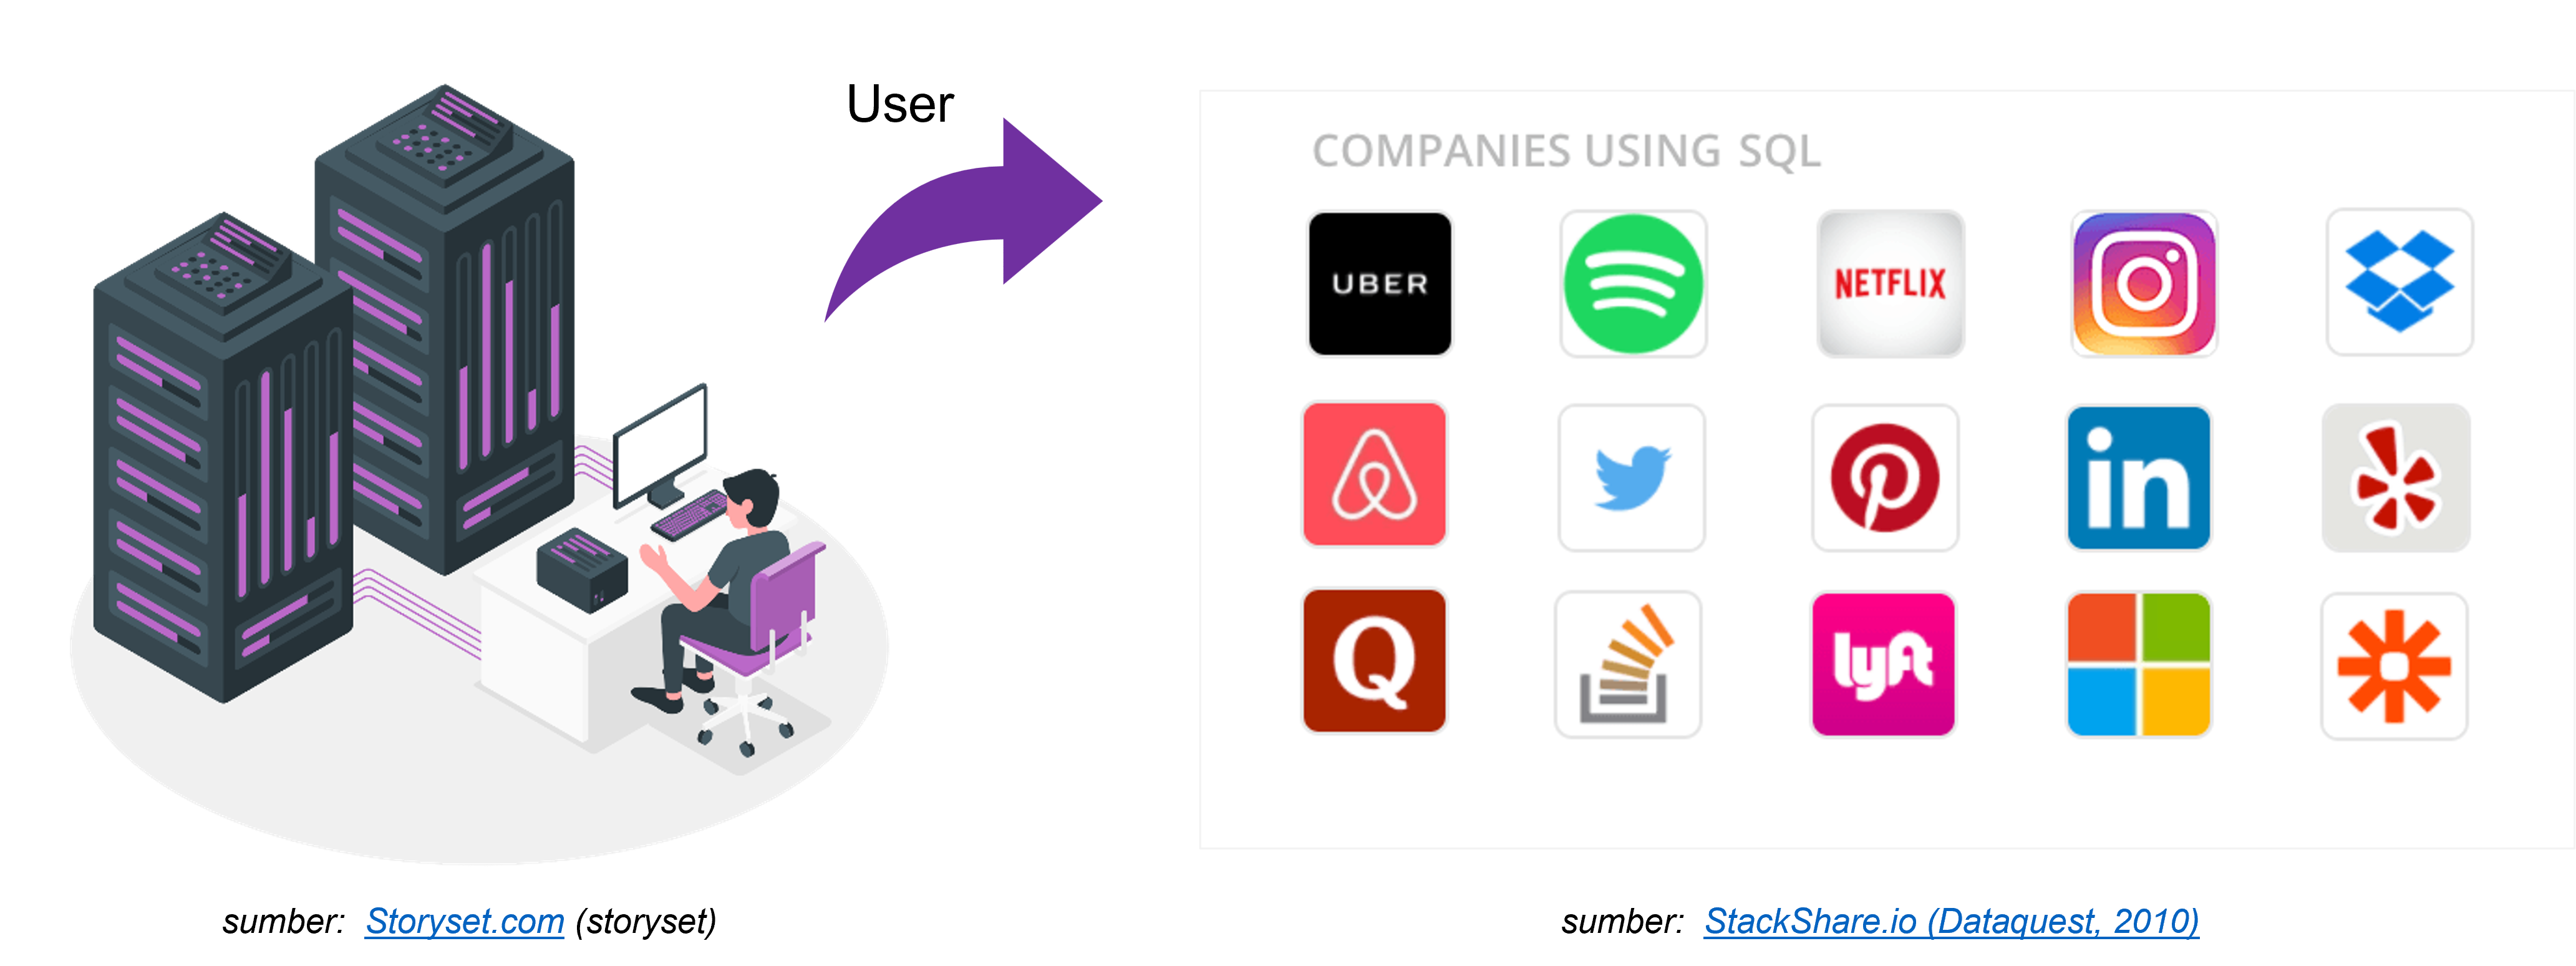
\includegraphics[width=1\linewidth]{./images/Bab1/SQL} 

}

\caption{Beberapa Perusahaan Besar Pengguna SQL}\label{fig:user-SQL}
\end{figure}

Banyak perusahaan besar di bidang teknologi menggunakan SQL seperti Uber, Netflix, dan Airbnb. Bahkan dalam perusahaan seperti Facebook, Google dan Amazon, yang telah membuat sendiri \textbf{SBD} berkemampuan tinggi, tetap menggunakan SQL untuk melakukan query dan analisis data.

\hypertarget{apa-itu-sbd}{%
\section{Apa itu SBD?}\label{apa-itu-sbd}}

Secara umum \textbf{SBD} dapat didefinisikan sebagai berikut:

\begin{figure}

{\centering 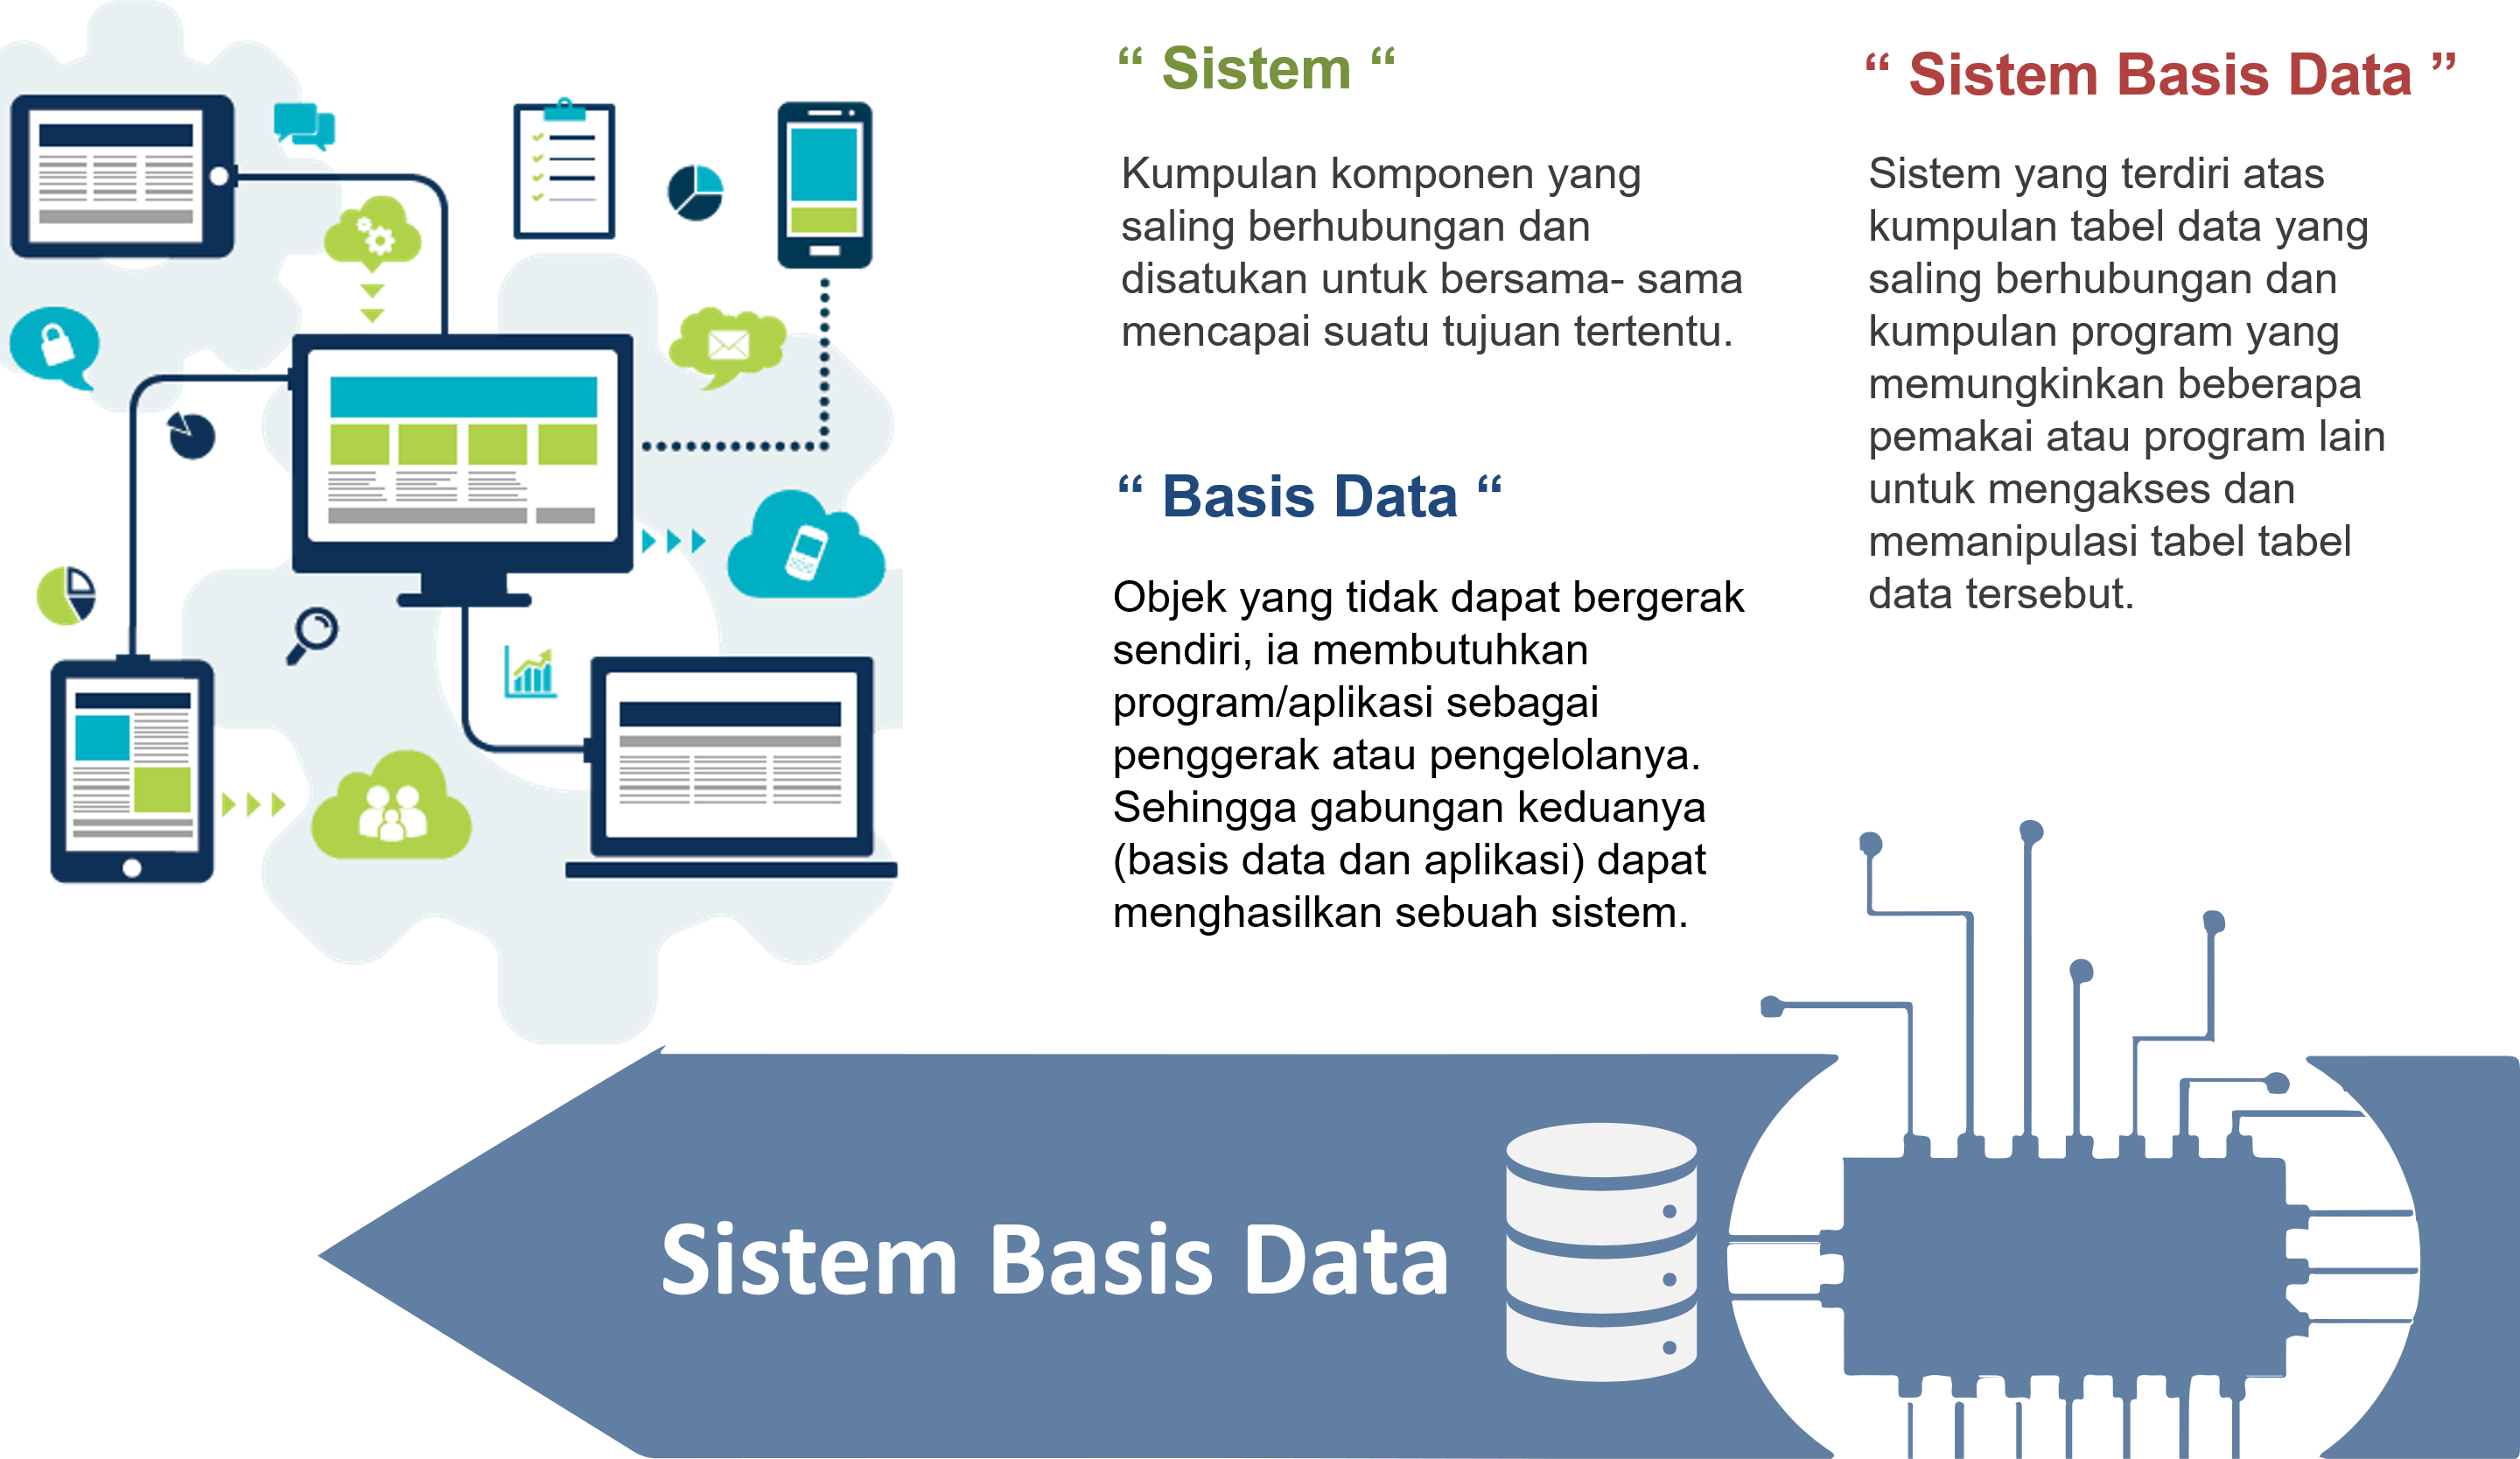
\includegraphics[width=1\linewidth]{./images/Bab1/definisi_DB} 

}

\caption{Definisi Sistem Basis Data}\label{fig:SBD}
\end{figure}

\hypertarget{komponen-sbd}{%
\subsection{Komponen SBD}\label{komponen-sbd}}

Adapun beberapa komponen dasar yang diperlukan dalam SBD adalah:

\begin{figure}

{\centering 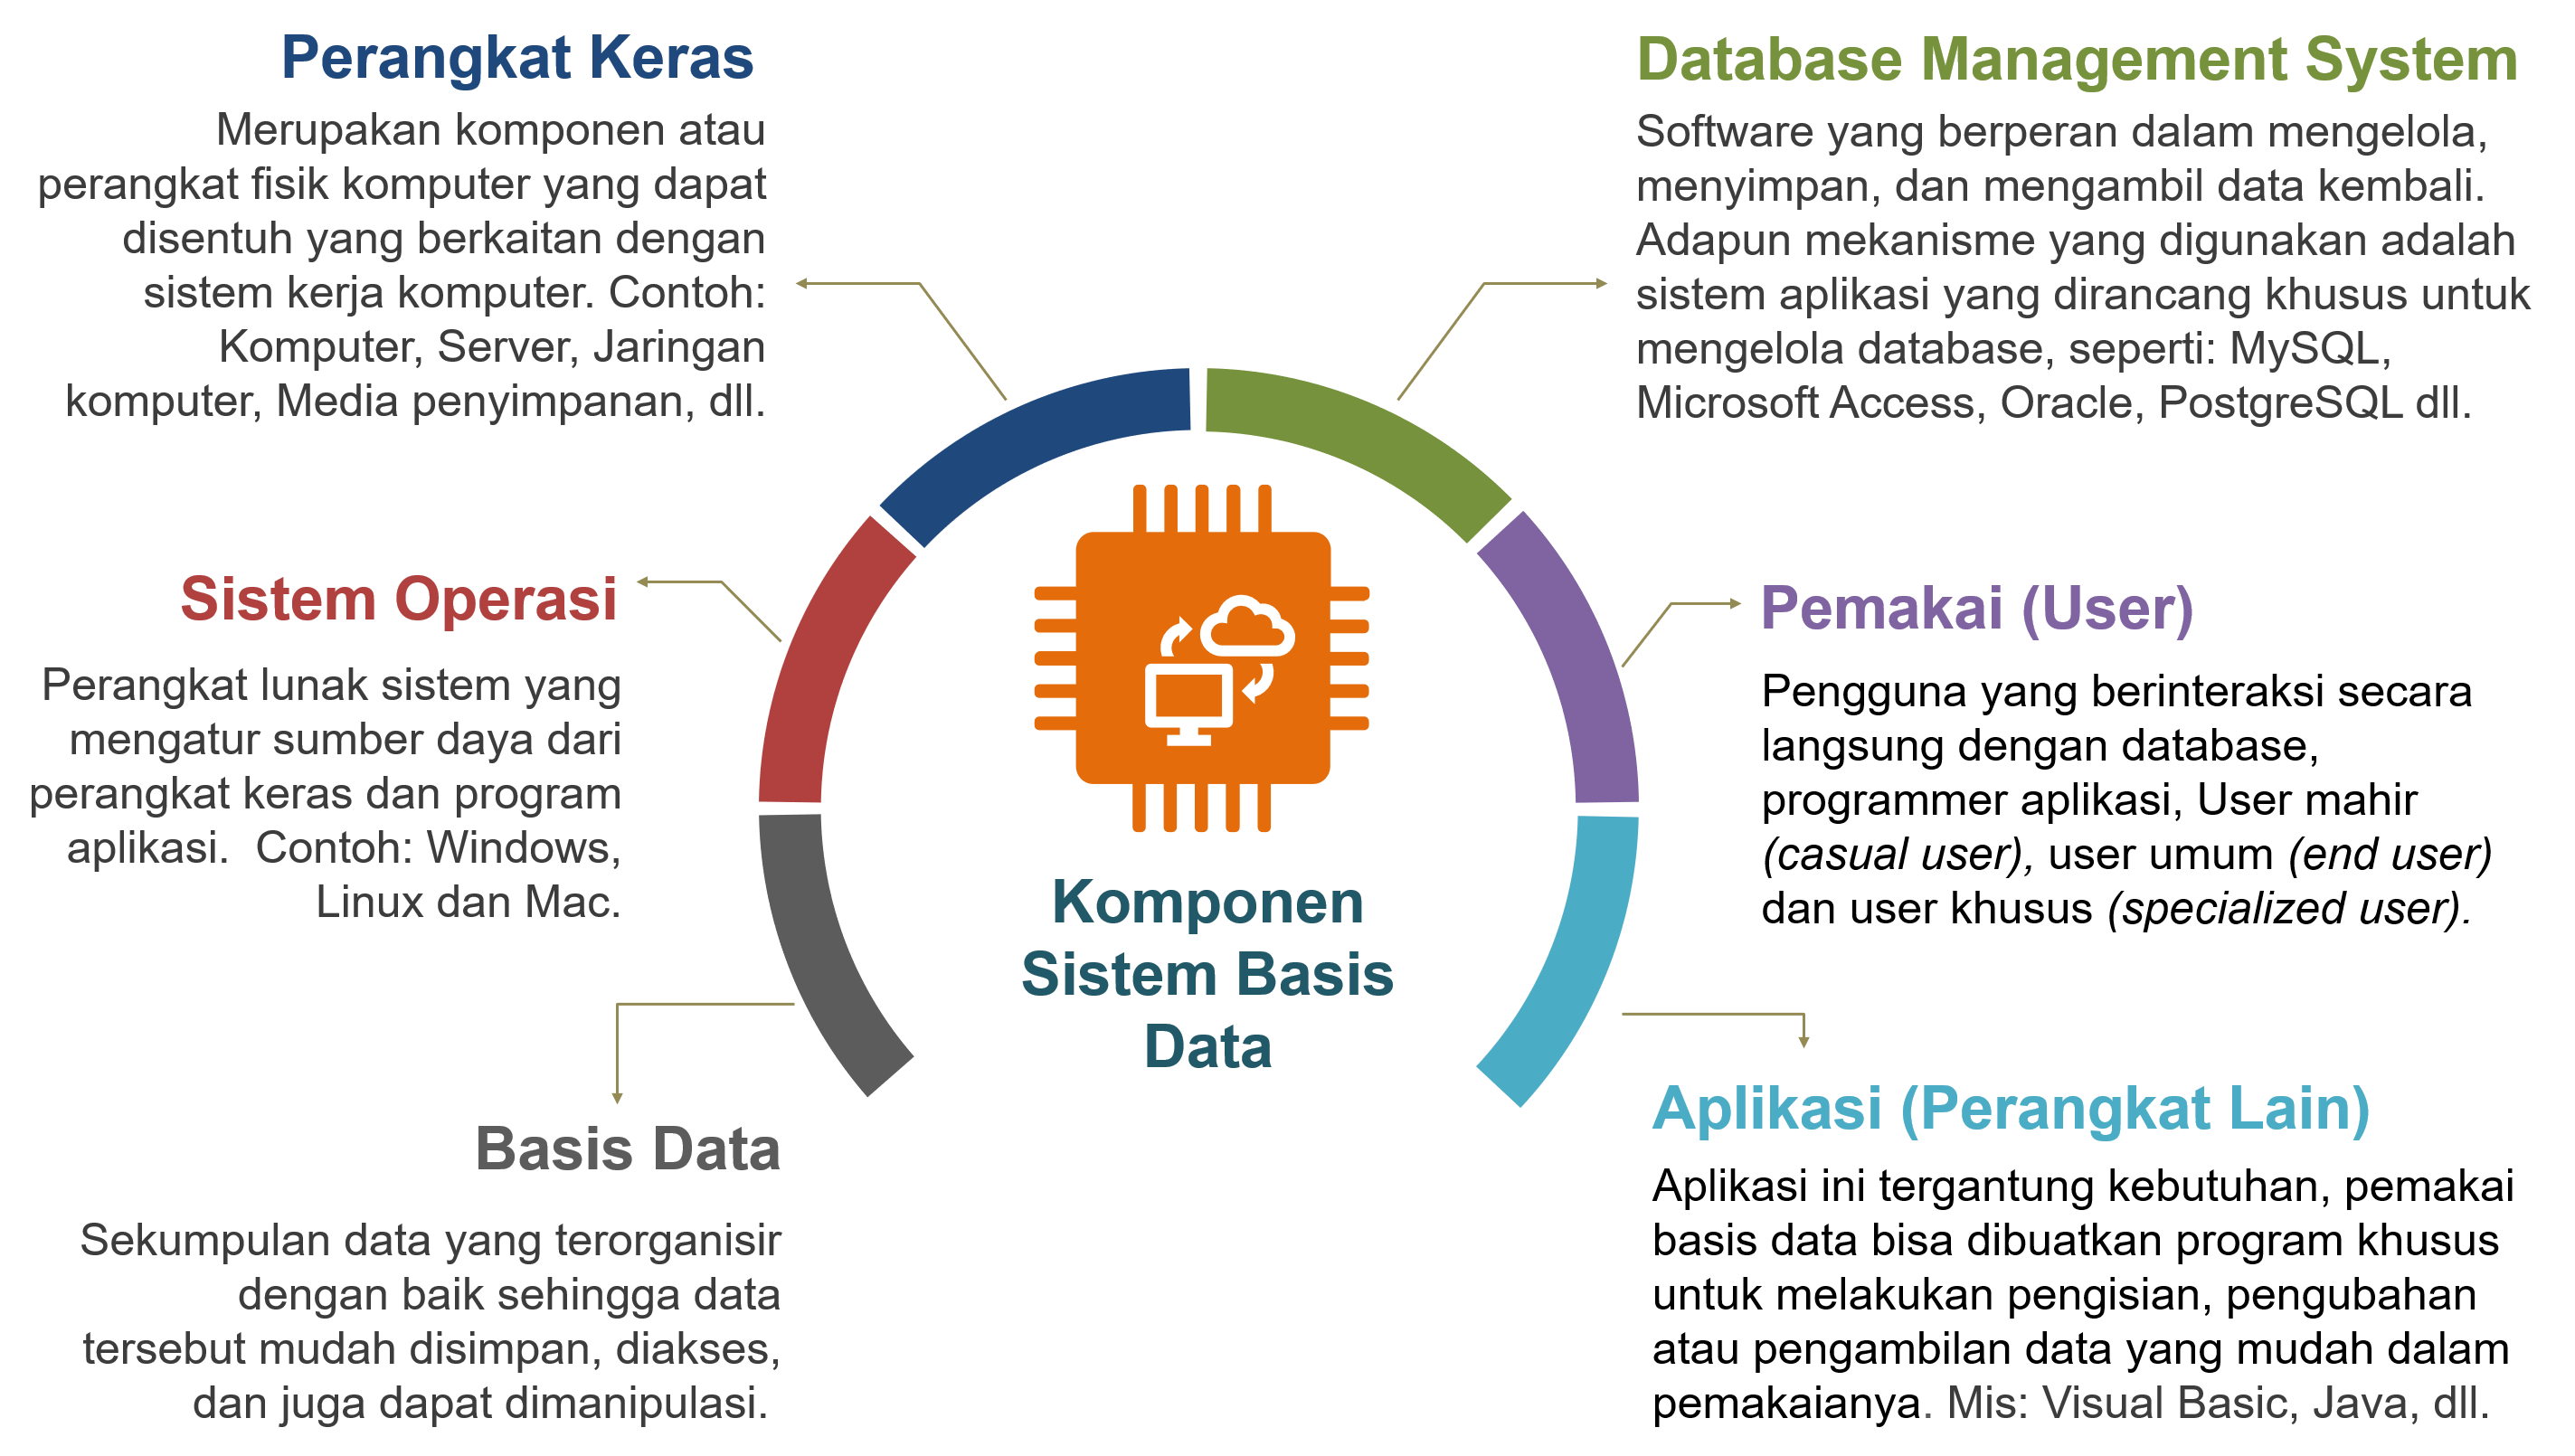
\includegraphics[width=1\linewidth]{./images/Bab1/komponen_DB} 

}

\caption{Komponen SBD}\label{fig:komponen}
\end{figure}

\begin{center}\rule{0.5\linewidth}{0.5pt}\end{center}

\hypertarget{manfaat-sbd}{%
\subsection{Manfaat SBD}\label{manfaat-sbd}}

Manfaat atau kegunaan penerapan SBD cukup banyak dan cakupannya pun luas dalam mendukung keberadaan lembaga atau organisasi maupun perusahaan, diantaranya:

\begin{figure}

{\centering 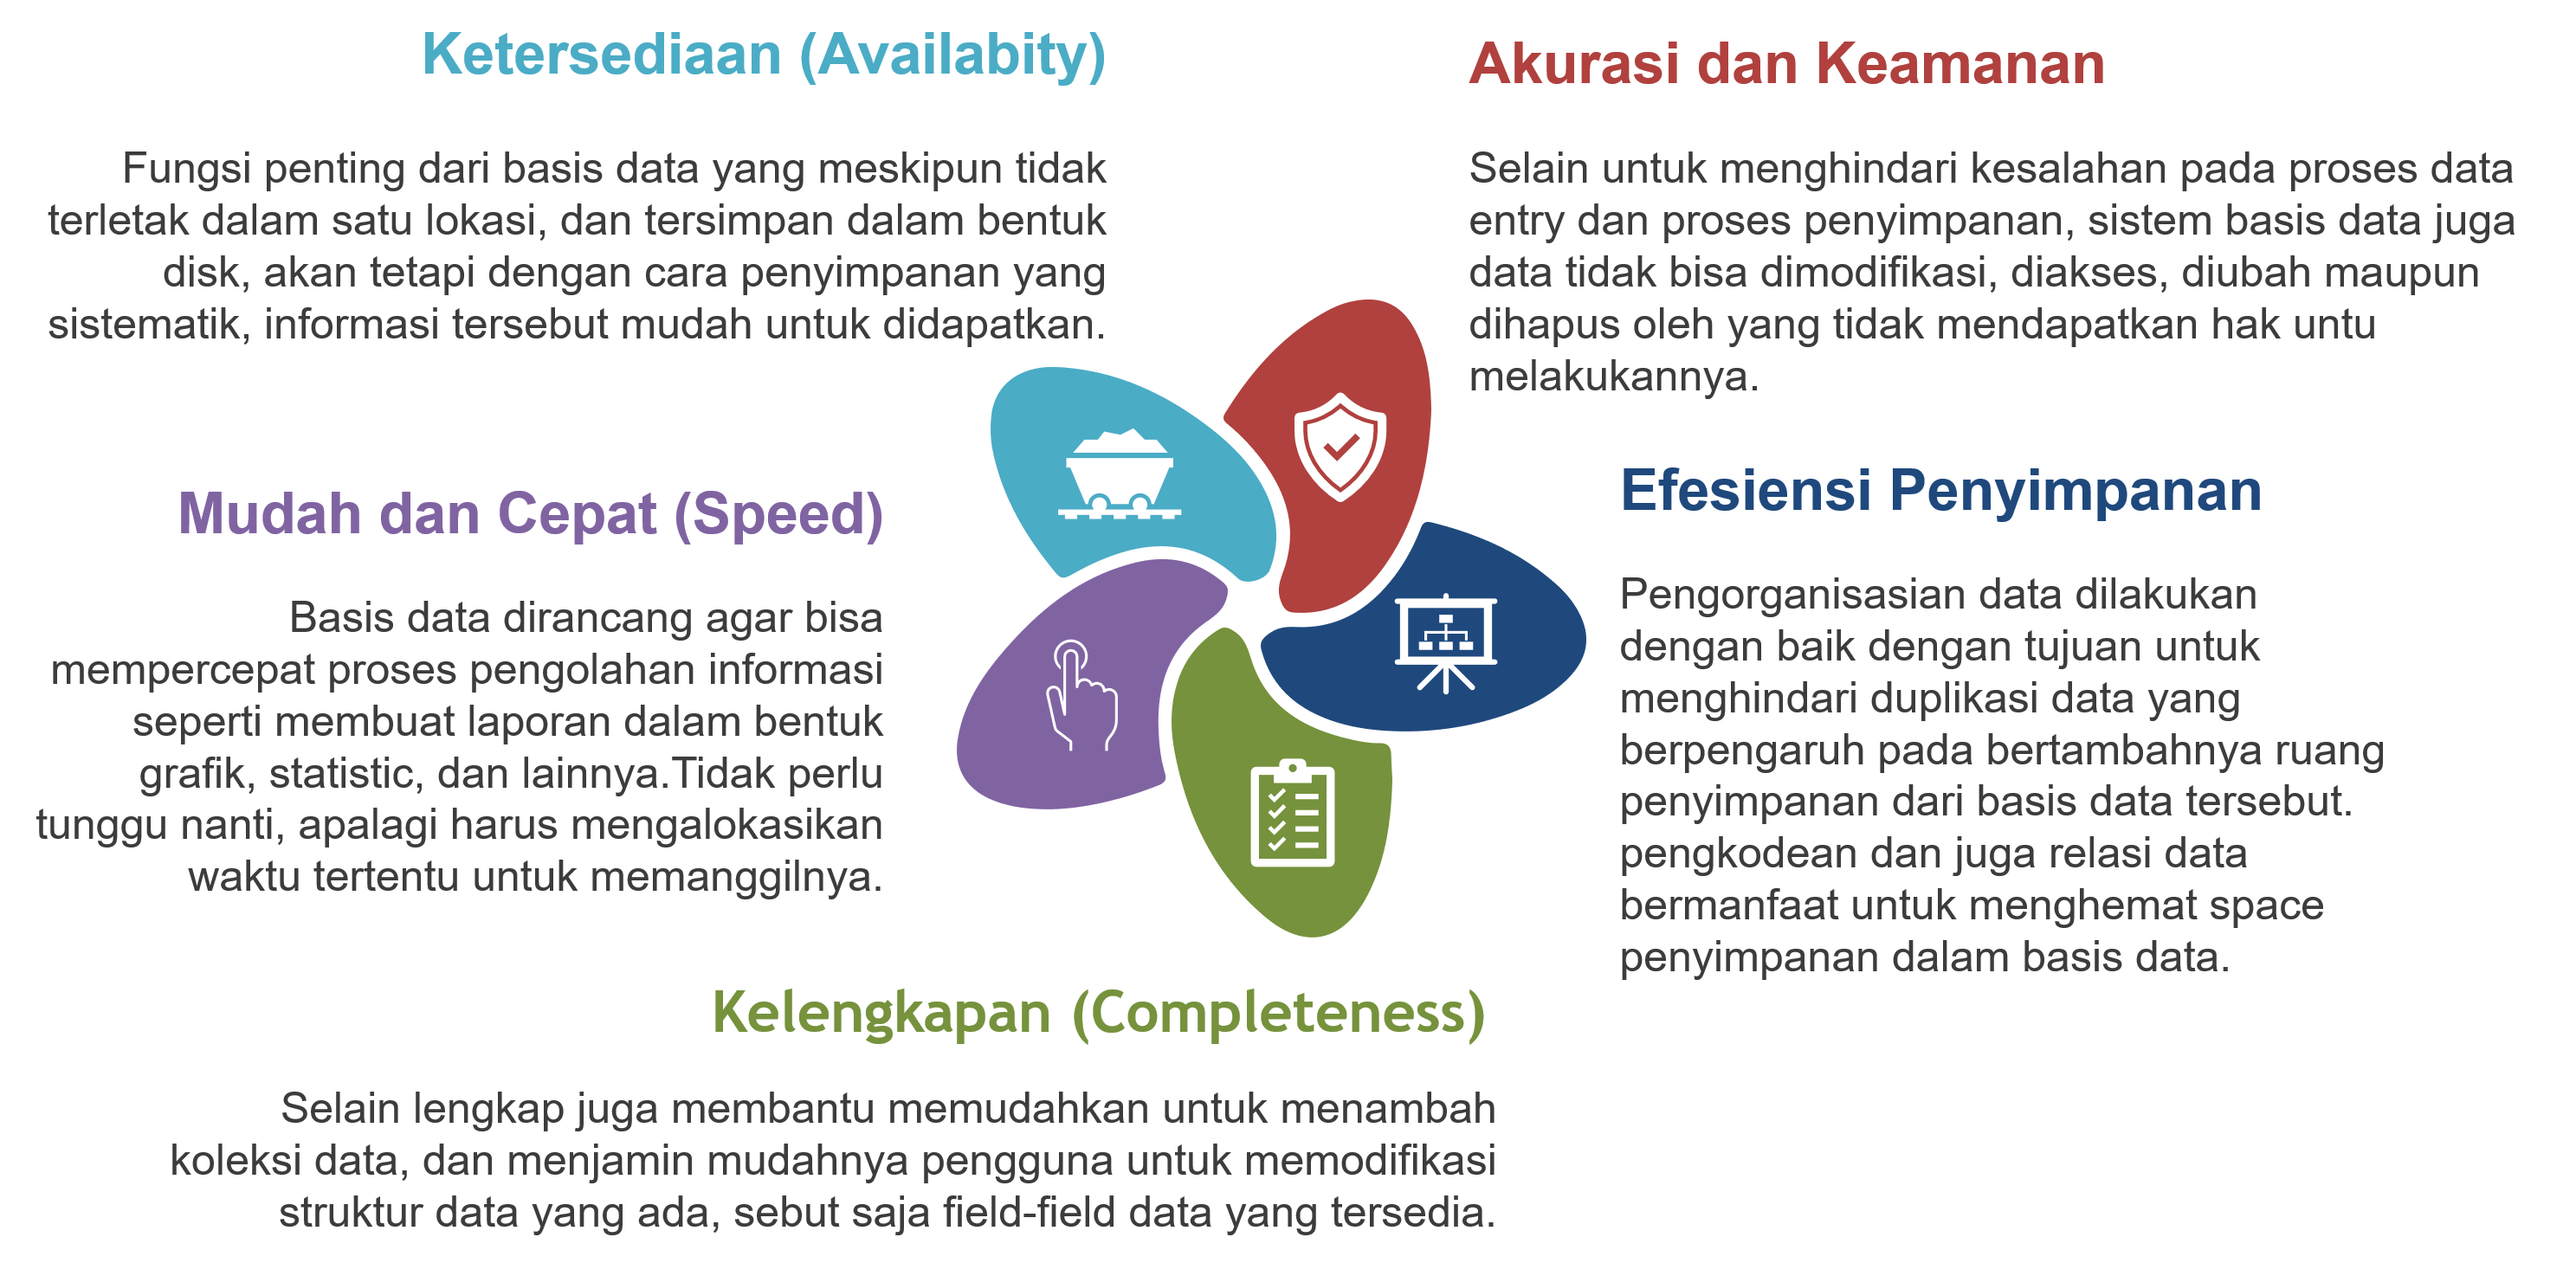
\includegraphics[width=1\linewidth]{./images/Bab1/manfaat_DB} 

}

\caption{Manfaat SBD}\label{fig:manfaat}
\end{figure}

\begin{center}\rule{0.5\linewidth}{0.5pt}\end{center}

\hypertarget{definisi-sql-vs-nosql}{%
\subsection{Definisi SQL vs NoSQL}\label{definisi-sql-vs-nosql}}

Sebenarnya perbedaan antara \href{https://www.dewaweb.com/blog/sql-pengertian-fungsi-beserta-perintah-dasarnya/}{SQL} dan \href{https://aws.amazon.com/id/nosql/}{NoSQL} secara mendasar sudah dapat dijelaskan dari akronimnya.

\begin{figure}

{\centering 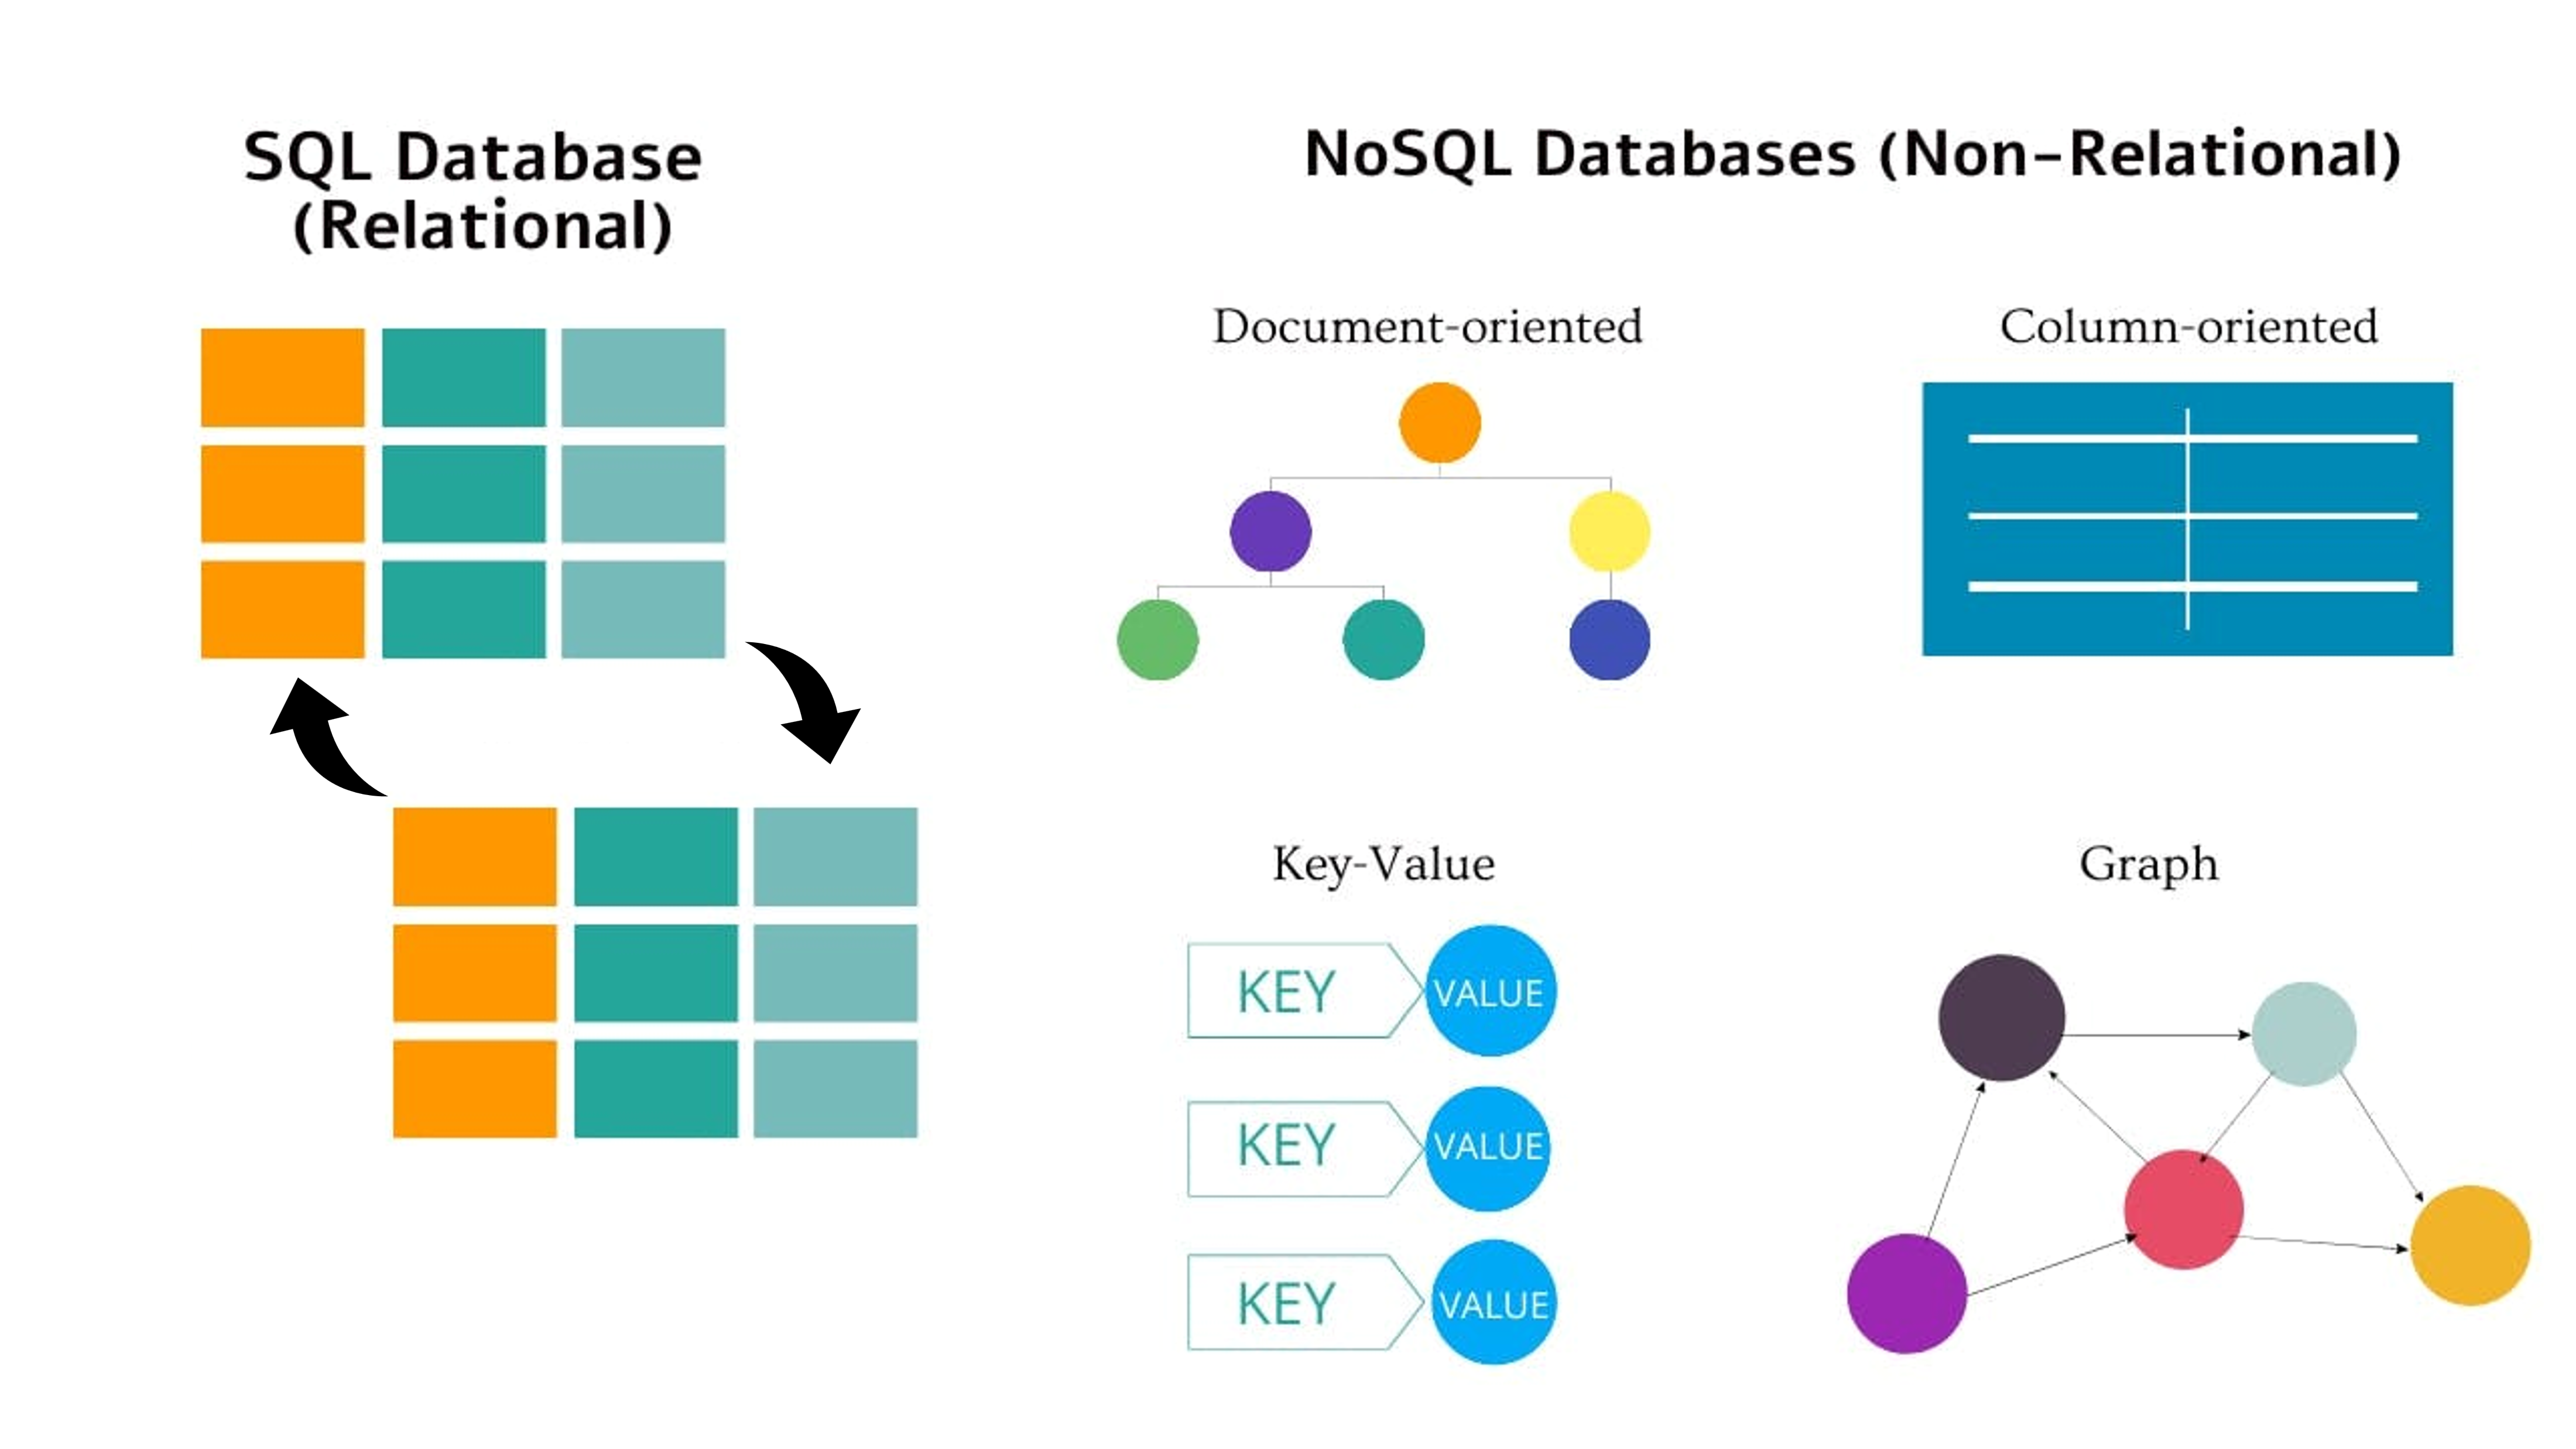
\includegraphics[width=1\linewidth]{./images/Bab1/SQLvsNoSQL_DB} 

}

\caption{SQL vs NoSQL}\label{fig:SQLvsNoSQL}
\end{figure}

\emph{SQL} basis data relasional yang menggunakan `relasi' (yang biasanya disebut tabel) untuk menyimpan data dan mencocokkan data tersebut dengan memakai karakteristik umum di setiap dataset. Sedangkan, \emph{NoSQL} adalah database yang menggunakan format JSON untuk setiap dokumennya sehingga mudah dibaca dan dimengerti. NoSQL banyak diminati karena memiliki performa yang tinggi dan bersifat non-relasional sehingga dapat memakai berbagai model data.

\begin{center}\rule{0.5\linewidth}{0.5pt}\end{center}

\hypertarget{perbedaan-sql-vs-nosql}{%
\subsection{Perbedaan SQL vs NoSQL}\label{perbedaan-sql-vs-nosql}}

Sebenarnya banyak perbedaan yang dimiliki di antara dua database tersebut tapi inilah perbedaan yang paling mencolok antara SQL dan NoSQL:

\begin{figure}

{\centering 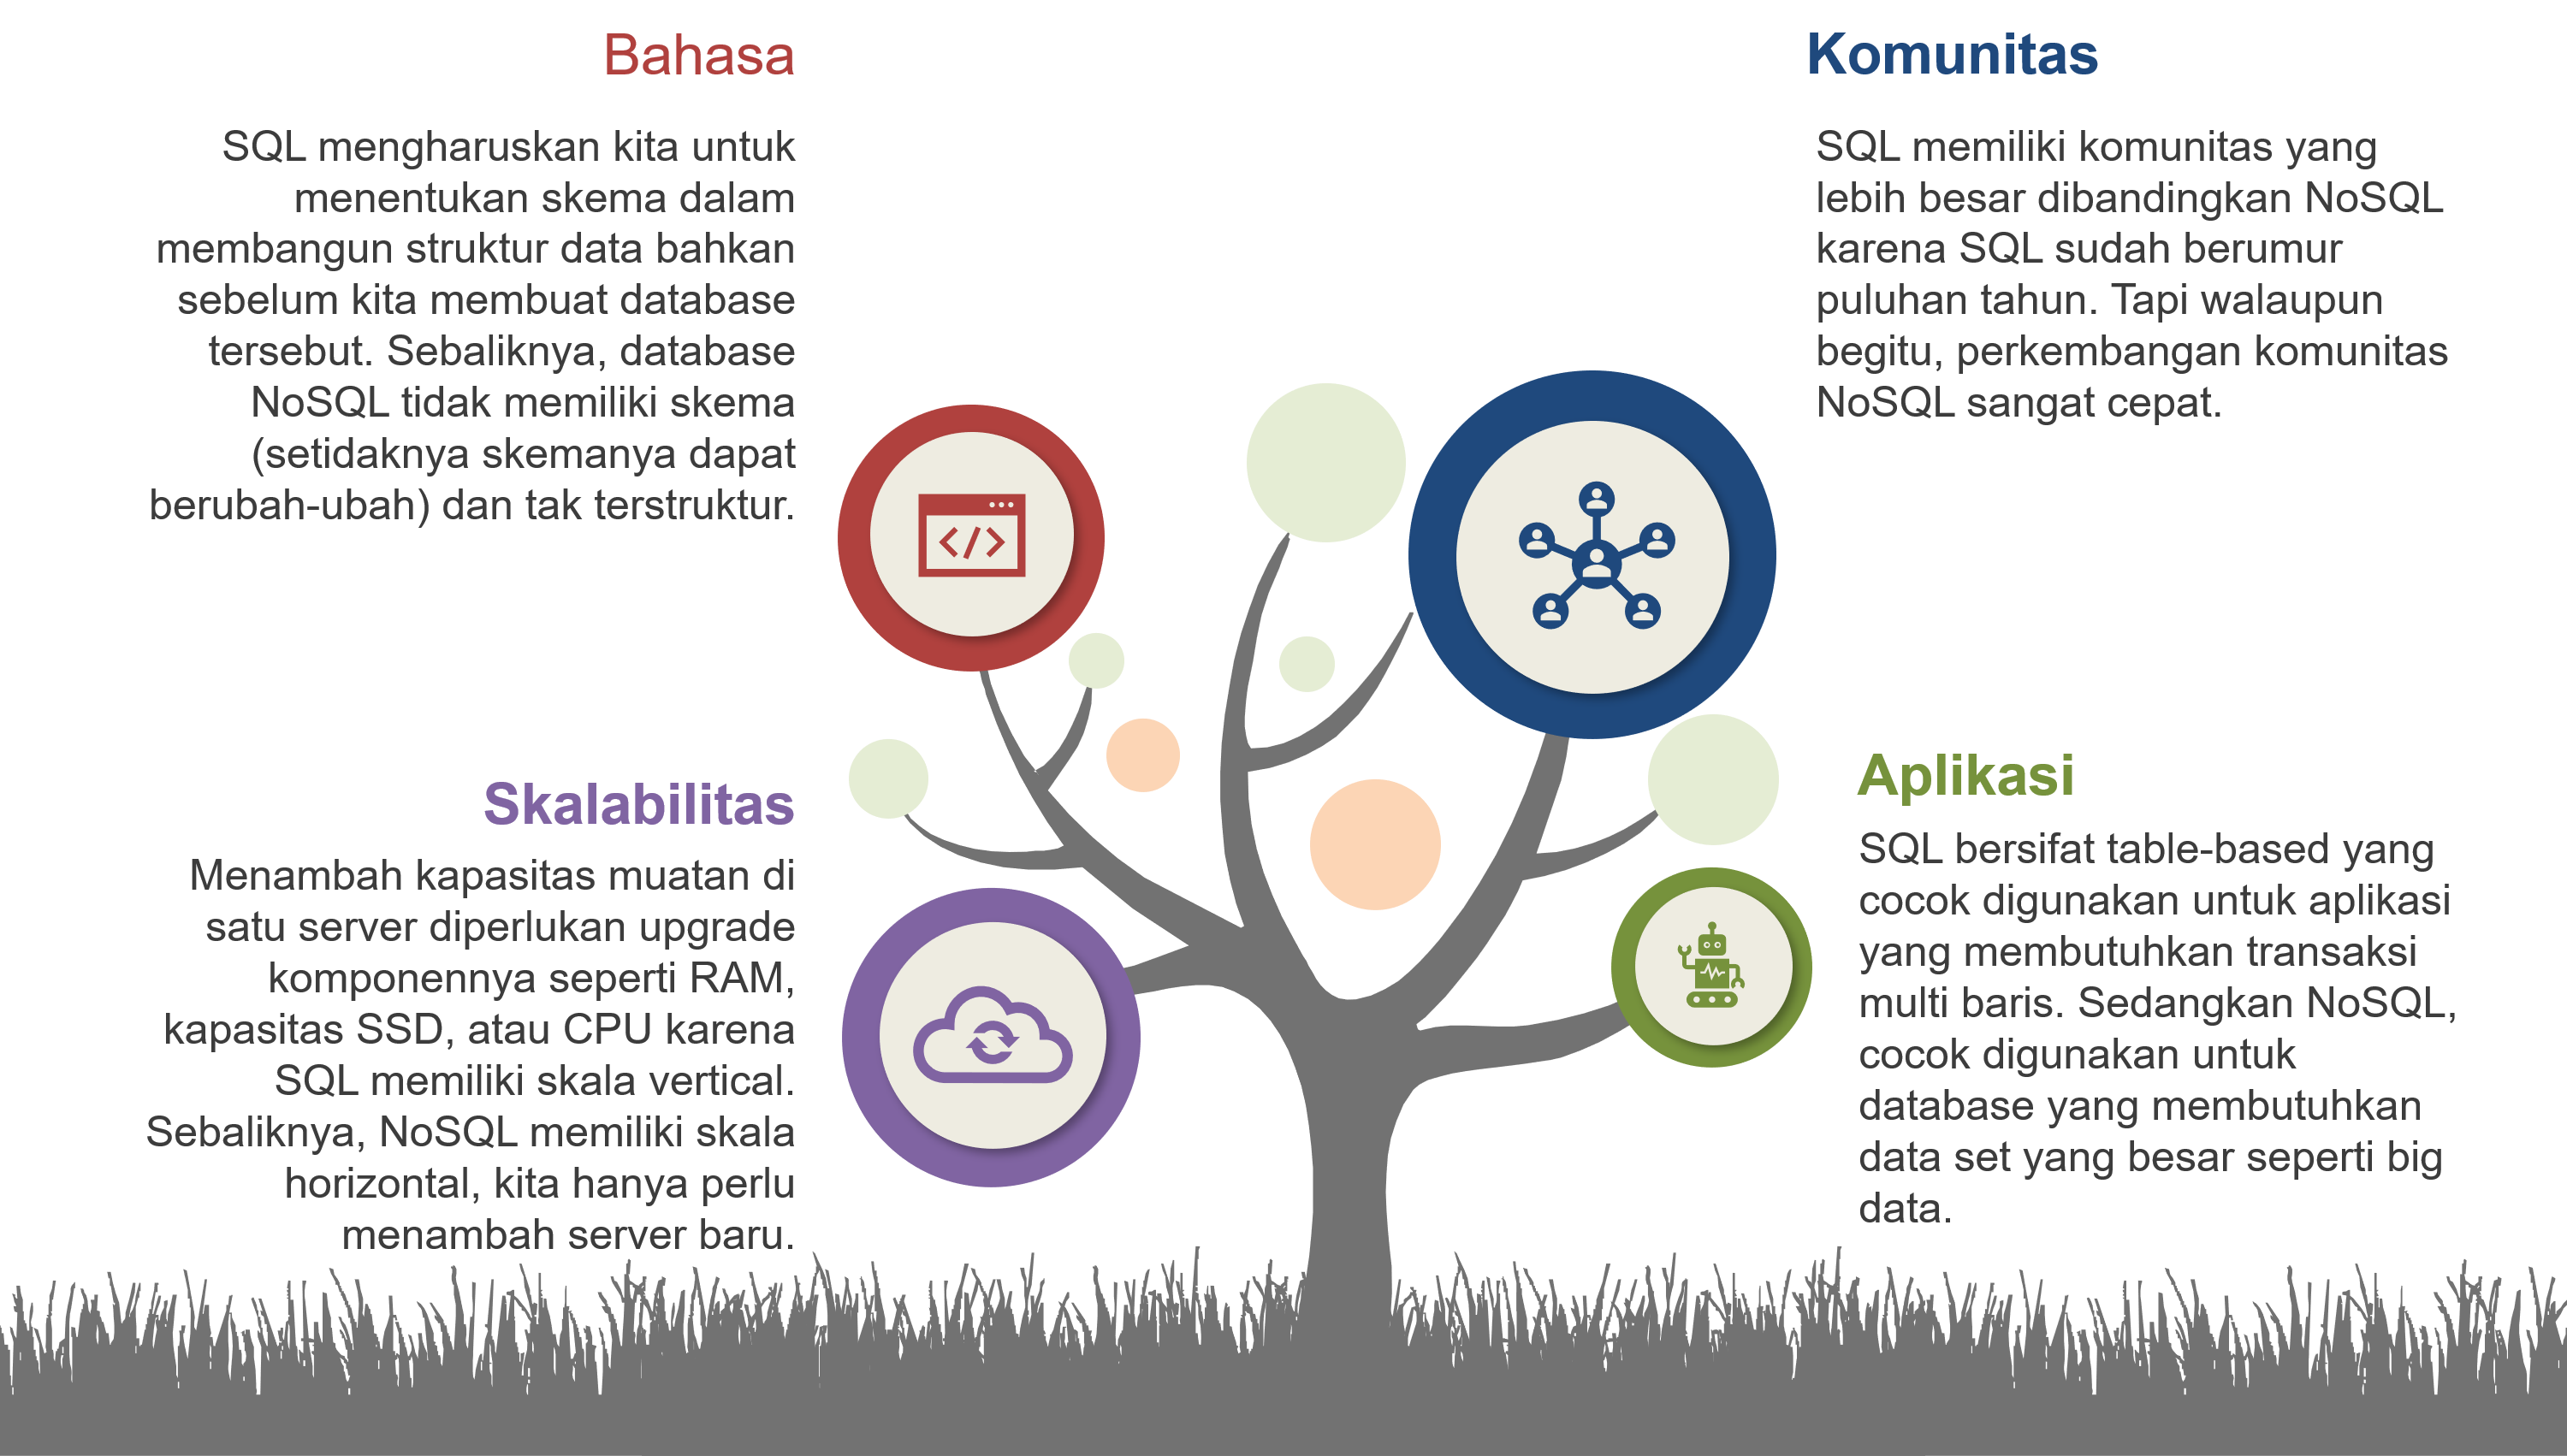
\includegraphics[width=1\linewidth]{./images/Bab1/Perbedaan_DB} 

}

\caption{Perbedaan SQL vs NoSQL}\label{fig:Perbedaan}
\end{figure}

\begin{center}\rule{0.5\linewidth}{0.5pt}\end{center}

\hypertarget{top-7-sql}{%
\subsection{Top 7 SQL}\label{top-7-sql}}

Tercatat sampai bulan Februari 2020 ada 334 jenis database menurut db-engines.com. Berikut ini saya merangkum daftar 7 database terpopuler yang menggunakan \href{https://qwords.com/blog/database-terpopuler/}{SQL} (Relasional):

\begin{figure}

{\centering 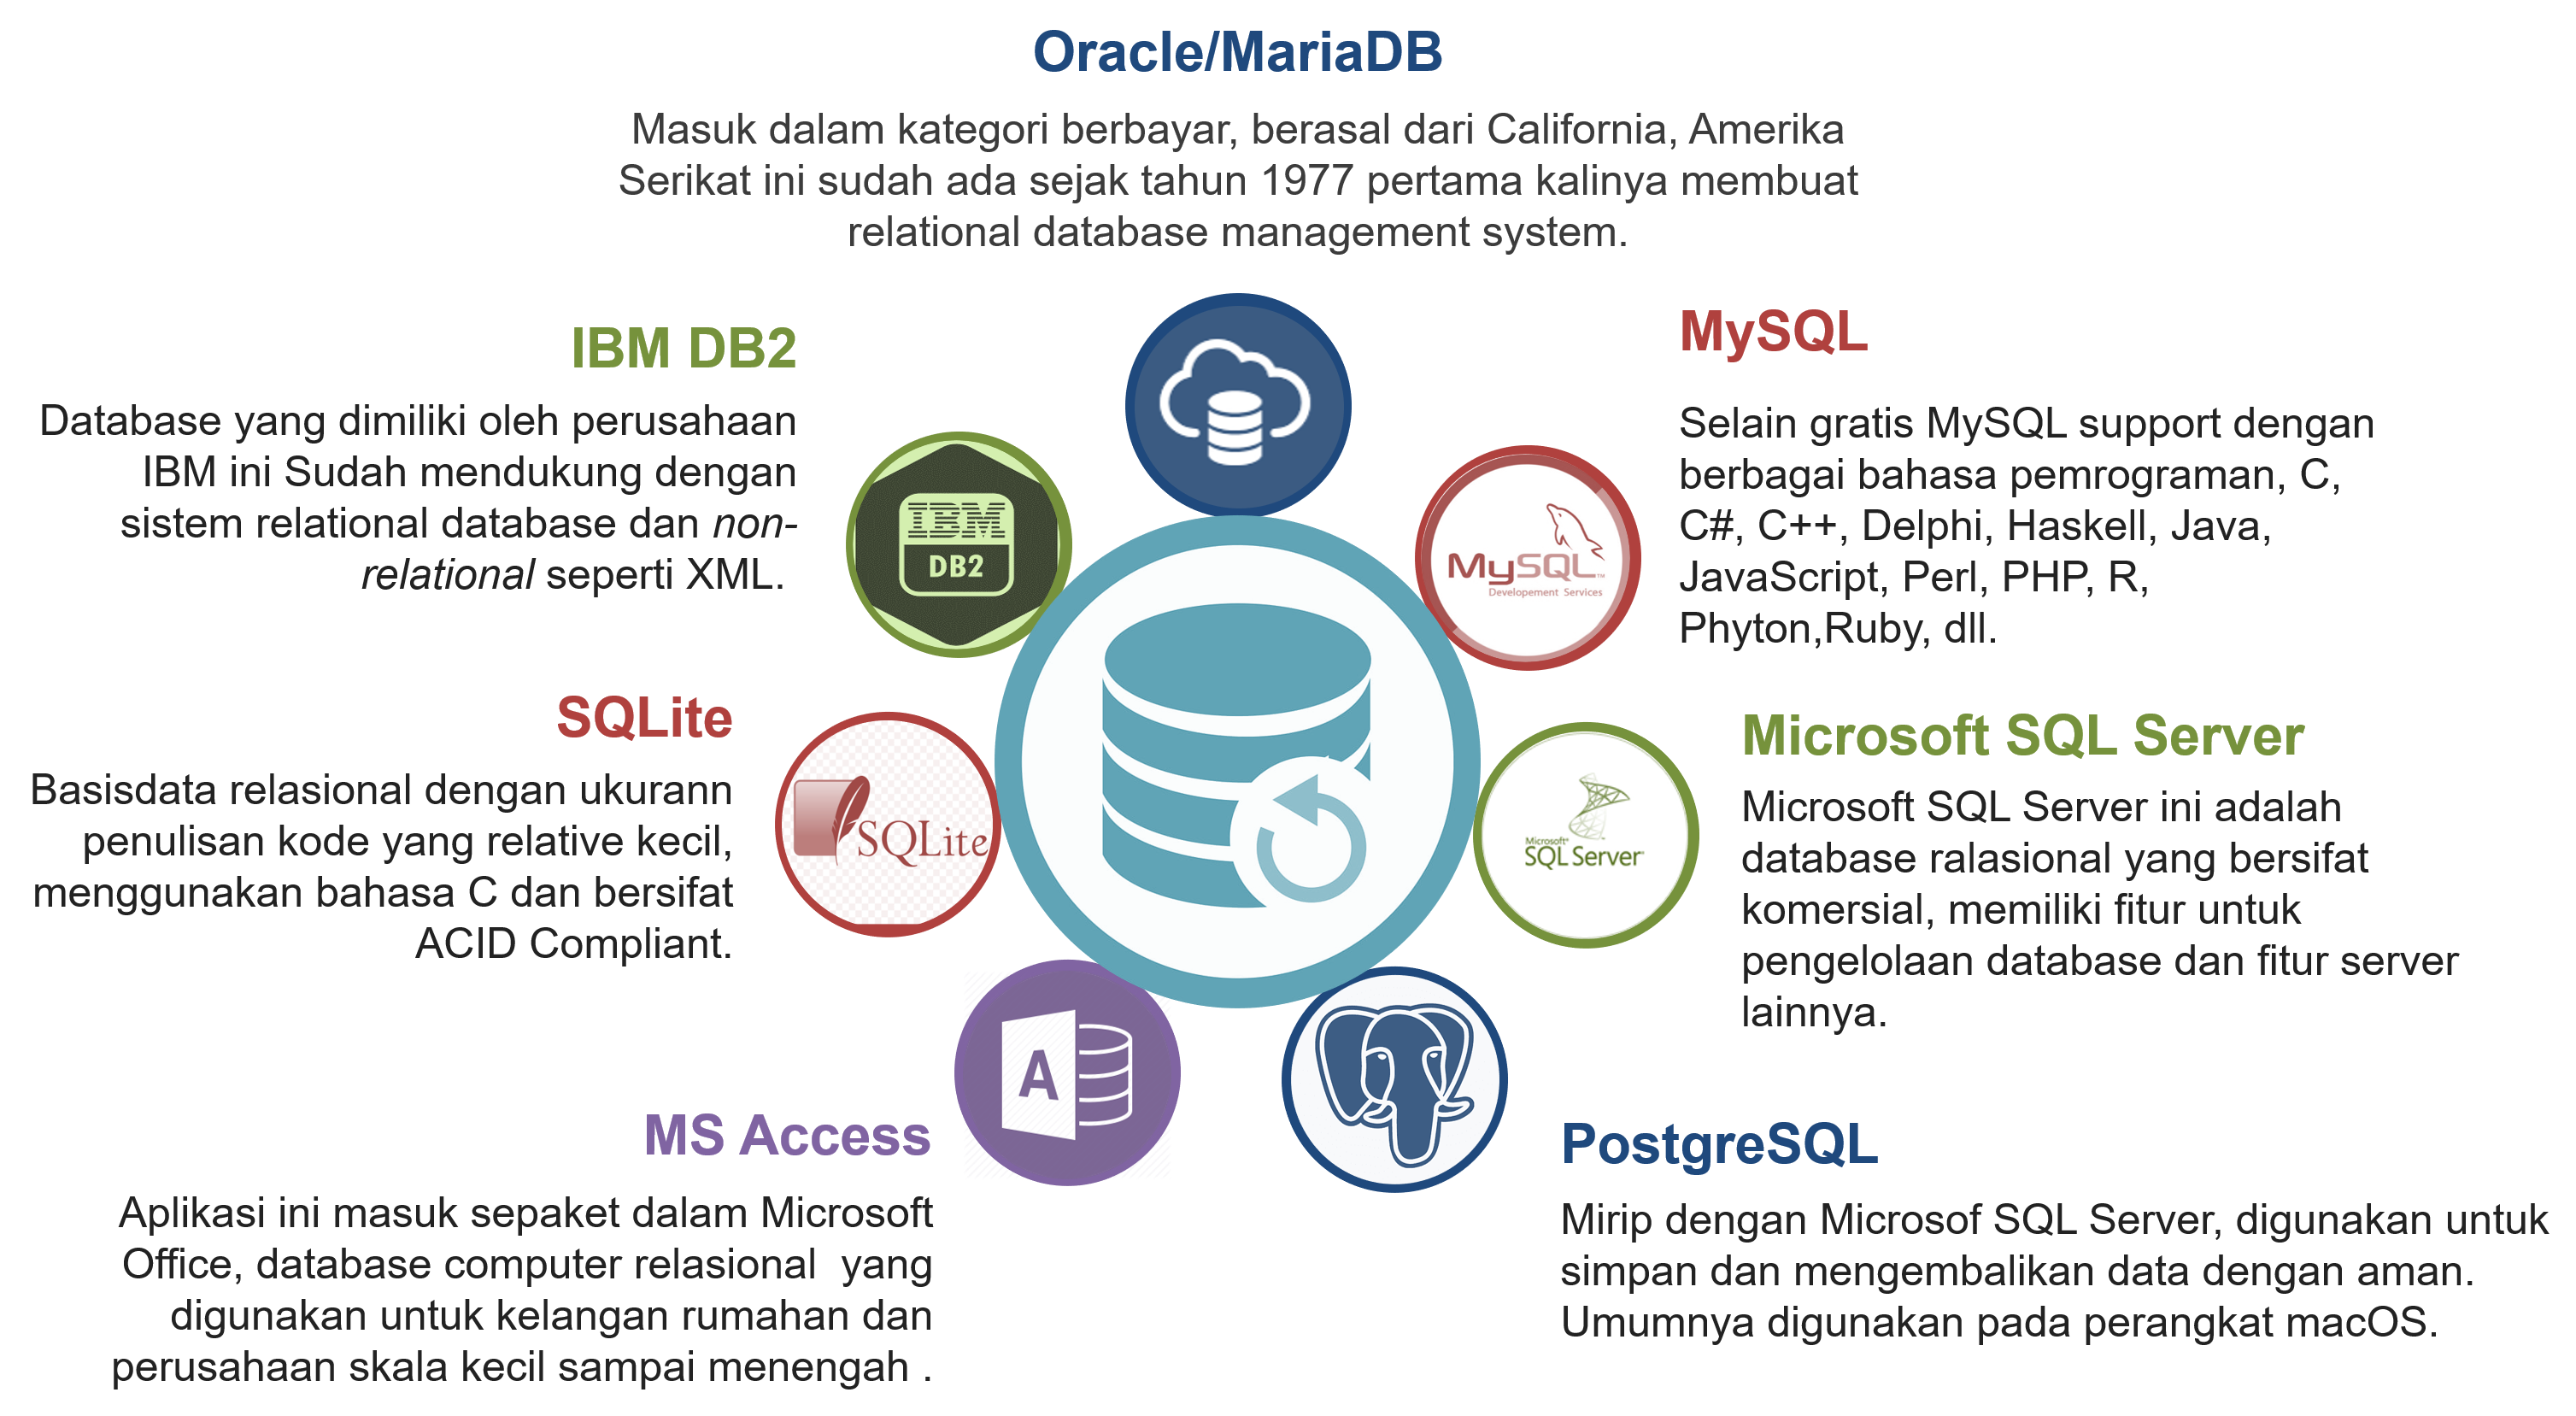
\includegraphics[width=1\linewidth]{./images/Bab1/7SQL_DB} 

}

\caption{Top 7 Perangkat Lunak SQL}\label{fig:top7SQL}
\end{figure}

\begin{center}\rule{0.5\linewidth}{0.5pt}\end{center}

\hypertarget{top-8-nosql}{%
\subsection{Top 8 NoSQL}\label{top-8-nosql}}

Kebanyakan basis data NoSQL digunakan dalam dunia aplikasi web waktu nyata (real-time web app). Berikut ini adalah ulasan 8 jenis basis data \href{https://www.codepolitan.com/7-basis-data-nosql-populer}{NoSQL} yang paling populer digunakan diseluruh dunia:

\begin{figure}

{\centering 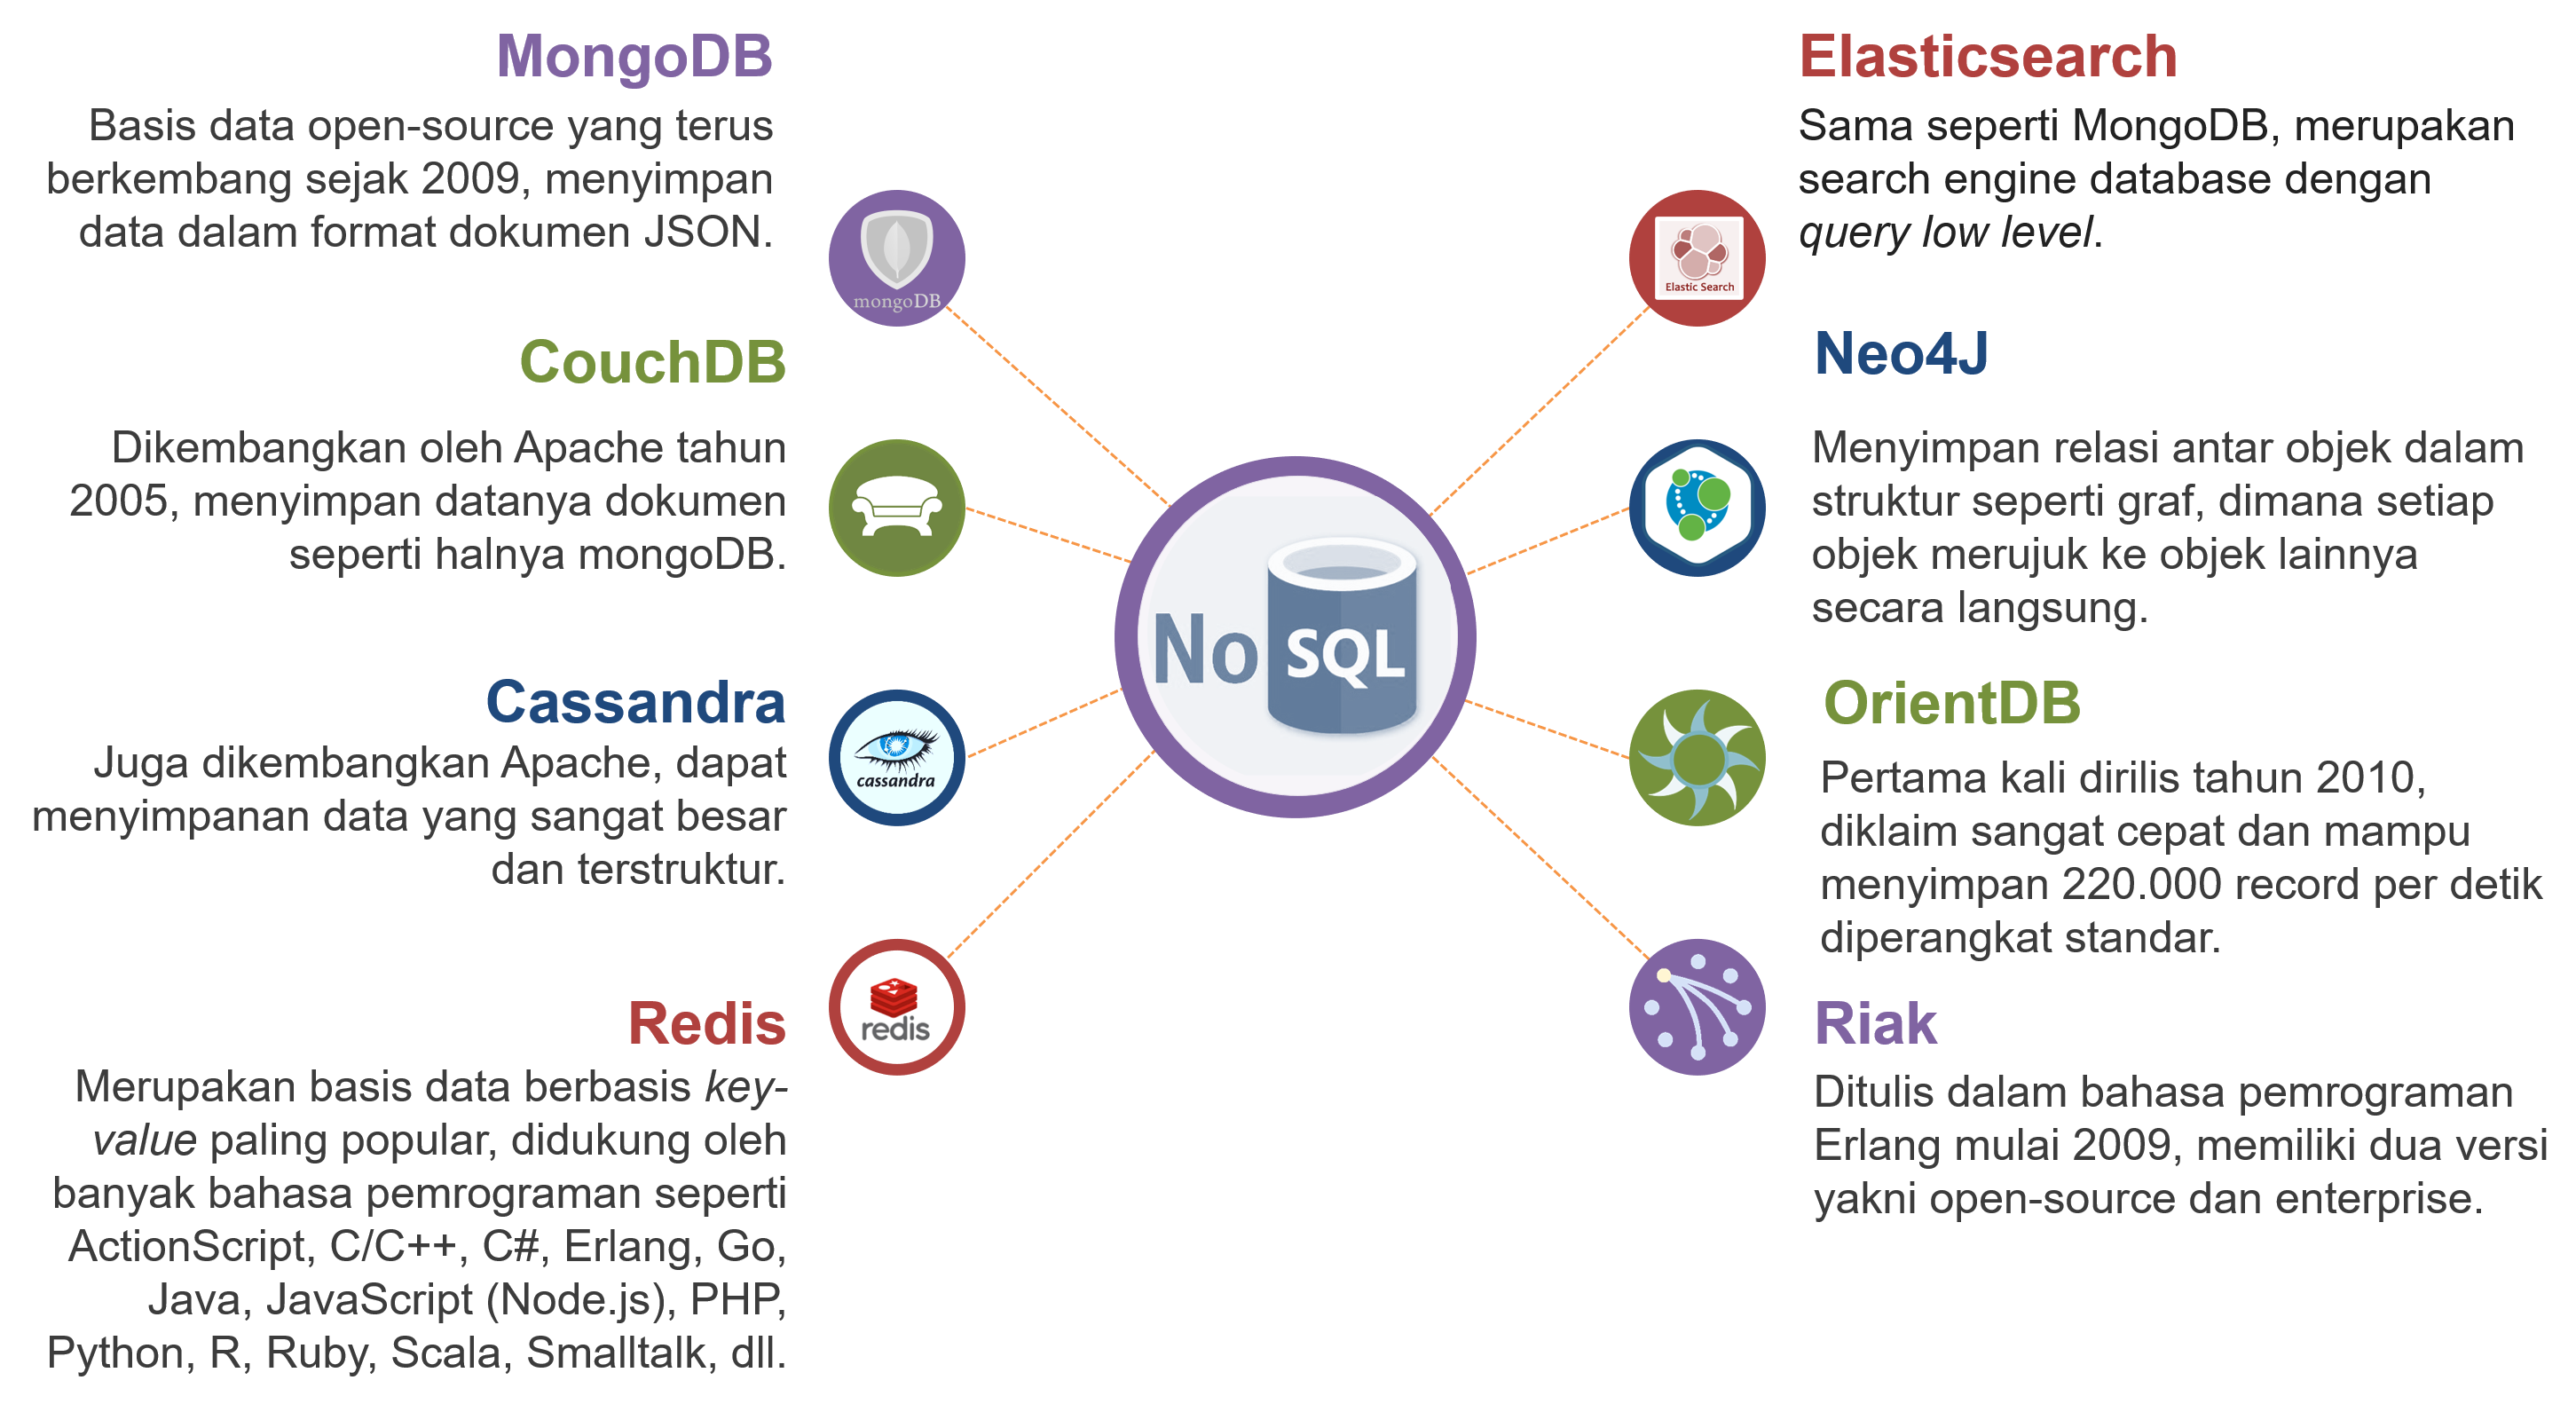
\includegraphics[width=1\linewidth]{./images/Bab1/8NoSQL_DB} 

}

\caption{Top 8 Perangkat Lunak NoSQL}\label{fig:top8noSQL}
\end{figure}

\begin{center}\rule{0.5\linewidth}{0.5pt}\end{center}

\hypertarget{mengapa-r-sql}{%
\section{Mengapa R \& SQL?}\label{mengapa-r-sql}}

Menggunakan R dan SQL merupakan kombinasi yang kuat untuk analisis data dan pengelolaan basis data. Keduanya memiliki peran yang berbeda dalam proses analisis dan pengelolaan data. Berikut adalah beberapa alasan mengapa menggunakan R dan SQL bersama:

\begin{itemize}
\tightlist
\item
  \textbf{Kekuatan Analisis R}
\end{itemize}

R adalah bahasa pemrograman yang khusus dirancang untuk analisis statistik dan visualisasi data.
R memiliki berbagai paket (packages) yang menawarkan fungsi statistik dan analisis yang kuat, termasuk regresi, pengelompokan, analisis deret waktu, dan banyak lagi.
Visualisasi yang dapat dihasilkan dengan R sangat bervariasi, dari grafik sederhana hingga visualisasi interaktif yang kompleks.

\begin{itemize}
\tightlist
\item
  \textbf{Manipulasi dan Pengelolaan Data dengan SQL}
\end{itemize}

SQL digunakan untuk mengelola dan mengambil data dari basis data terstruktur.
SQL menyediakan cara efisien untuk membuat, mengubah, menghapus, dan memanipulasi data dalam basis data.
SQL memiliki fitur untuk menggabungkan data dari berbagai tabel, melakukan agregasi, dan menyaring data.

\begin{itemize}
\tightlist
\item
  \textbf{Integrasi Antara R dan SQL}
\end{itemize}

Banyak perpustakaan R yang mendukung koneksi ke basis data menggunakan SQL.
Anda dapat menggunakan perintah SQL dalam skrip R untuk mengambil data dari basis data, memanipulasi data di dalam R, dan kemudian menerapkan analisis statistik menggunakan paket R. Integrasi ini memungkinkan Anda menggabungkan kekuatan analisis statistik R dengan kemampuan pengelolaan data SQL.

\begin{itemize}
\tightlist
\item
  \textbf{Skalabilitas dan Efisiensi}
\end{itemize}

Menggunakan SQL untuk mengambil dan memanipulasi data dalam basis data bisa lebih efisien daripada melakukannya dalam R, terutama untuk dataset besar.
SQL memungkinkan query yang dioptimalkan dan penggunaan indeks untuk kinerja yang lebih baik.

\begin{itemize}
\tightlist
\item
  \textbf{Data Preprocessing}
\end{itemize}

Sebelum menerapkan analisis di R, Anda mungkin perlu melakukan pra-pemrosesan pada data, seperti membersihkan data, menggabungkan tabel, dan mengisi data yang hilang. SQL dapat membantu dalam melakukan tugas-tugas ini.

Jadi, menggunakan R dan SQL bersama memungkinkan Anda menggabungkan kekuatan analisis statistik R dengan kemampuan pengelolaan data SQL. Ini bisa sangat berguna ketika Anda ingin melakukan analisis data yang luas dan kompleks dari berbagai sumber data yang berbeda.

\begin{figure}

{\centering 
\includegraphics[width=1\linewidth]{./images/Bab1/sql-r-friends} 

}

\caption{R dan SQL [https://irene.rbind.io](https://irene.rbind.io/post/using-sql-in-rstudio/)}\label{fig:sql-r-friends}
\end{figure}

\hypertarget{mysql-vs-postgresql}{%
\section{MySQL vs PostgreSQL}\label{mysql-vs-postgresql}}

MySQL adalah sistem manajemen basis data relasional yang memungkinkan Anda untuk menyimpan data sebagai tabel dengan baris dan kolom. Sistem ini populer sehingga digunakan di banyak aplikasi web, situs web dinamis, dan sistem tertanam. PostgreSQL adalah sistem manajemen basis data relasional-objek yang menawarkan lebih banyak fitur daripada MySQL. Sistem ini memberi Anda lebih banyak fleksibilitas dalam tipe data, skalabilitas, konkurensi, dan integrasi data.

\begin{figure}

{\centering 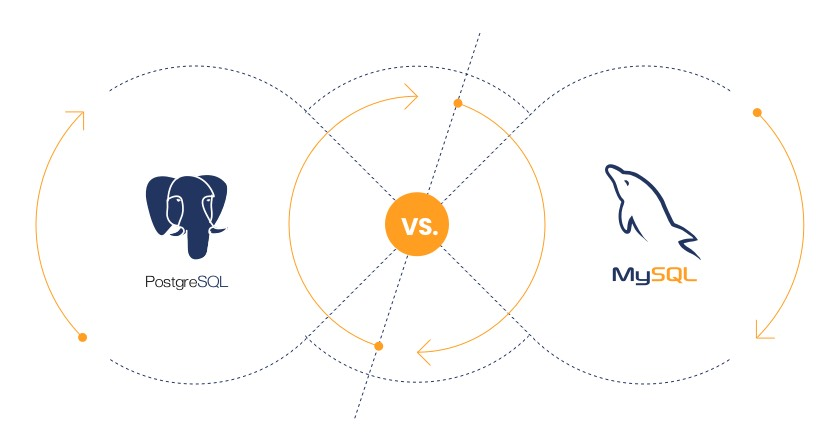
\includegraphics[width=1\linewidth]{./images/Bab1/MySQL-VS-PostgreSQL} 

}

\caption{MySQL vs PostgreSQL [https://integrio.net/](https://integrio.net/blog/postgresql-vs-mysql)}\label{fig:MySQL-VS-PostgreSQL}
\end{figure}

MySQL dan PostgreSQL, Keduanya menyimpan data di dalam tabel yang terkait satu sama lain melalui nilai kolom umum. Namun keduanya sering dibandingkan karena terdapat beberapa perbedaan. Ingin mengenal lebih dalam? Simak penjelasan di bawah.

\hypertarget{kelebihan}{%
\subsection{Kelebihan}\label{kelebihan}}

\begin{longtable}[]{@{}
  >{\raggedright\arraybackslash}p{(\columnwidth - 2\tabcolsep) * \real{0.4545}}
  >{\raggedright\arraybackslash}p{(\columnwidth - 2\tabcolsep) * \real{0.5455}}@{}}
\toprule\noalign{}
\begin{minipage}[b]{\linewidth}\raggedright
MySQL
\end{minipage} & \begin{minipage}[b]{\linewidth}\raggedright
PostgreSQL
\end{minipage} \\
\midrule\noalign{}
\endhead
\bottomrule\noalign{}
\endlastfoot
Integrasi bahasa pemrograman sangat luas; & Support framework website modern seperti Node.js dan Django; Support framework website modern seperti Node.js dan Django; \\
Aplikasi ringan, tidak membutuhkan spesifikasi hardware yang tinggi; & Dirilis dengan lisensi PostgreSQL sendiri; \\
Struktur tabel dengan fleksibilitas tinggi; & Bersifat open source dan gratis; \\
Dibekali banyak administrative tools; & Skala besar, mampu memuat hingga ribuan transaksi data; \\
Bersifat open source dan gratis (versi basic); & Memiliki banyak fitur yang mumpuni; \\
Meski open source, MySQL menjamin keamanan tingkat tinggi; & Memiliki banyak fitur yang mumpuni; \\
Mendukung berbagai variasi Data Type; & Performa sangat baik meski menuntut query yang lebih kompleks; \\
Dapat digunakan banyak pengguna karena mendukung multi user. & Kecepatan analisis (read-write) sangat cepat; Keamanan yang lebih ketat. \\
\end{longtable}

\hypertarget{kekurangan}{%
\subsection{Kekurangan}\label{kekurangan}}

\begin{longtable}[]{@{}
  >{\raggedright\arraybackslash}p{(\columnwidth - 2\tabcolsep) * \real{0.4545}}
  >{\raggedright\arraybackslash}p{(\columnwidth - 2\tabcolsep) * \real{0.5455}}@{}}
\toprule\noalign{}
\begin{minipage}[b]{\linewidth}\raggedright
MySQL
\end{minipage} & \begin{minipage}[b]{\linewidth}\raggedright
PostgreSQL
\end{minipage} \\
\midrule\noalign{}
\endhead
\bottomrule\noalign{}
\endlastfoot
Sistem manajemen database kurang cocok untuk aplikasi mobile dan game; & PostgreSQL tidak mendukung semua stack development; \\
Technical support MySQL dinilai kurang baik; & Meski memiliki integrasi dan skalabilitas tinggi, kecepatan PostgreSQL kalah unggul dibandingkan RDBMS lain; \\
Sulit diaplikasikan untuk manajemen database berskala besar. & Sistem kompatibilitas PostgreSQL menuntut pengguna untuk bekerja lebih keras dalam perbaikan dan perawatan. \\
\end{longtable}

\hypertarget{instalasi-mysql-xampp}{%
\section{Instalasi MySQL (XAMPP)}\label{instalasi-mysql-xampp}}

\hypertarget{download-aplikasi-xampp}{%
\subsection{Download Aplikasi XAMPP}\label{download-aplikasi-xampp}}

Silakan \href{https://www.apachefriends.org/download.html}{klik disini} untuk mengunduh applikasi XAMPP, pilih salah satu saja sesuai Operating System pada Komputer anda.

\begin{figure}

{\centering 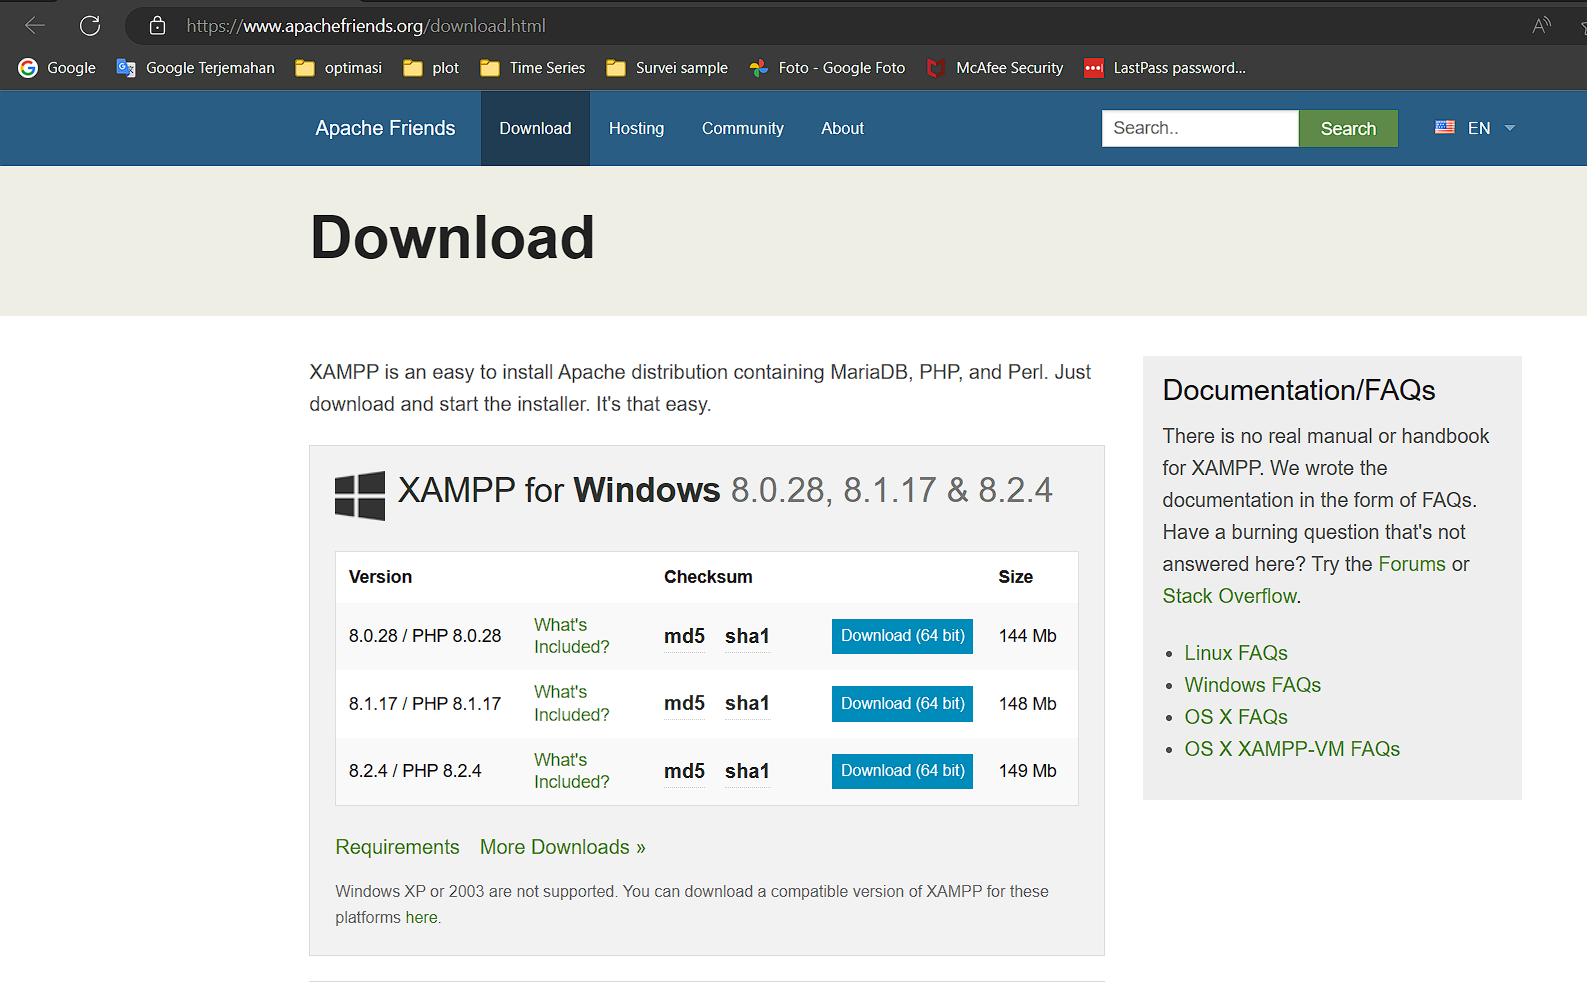
\includegraphics[width=1\linewidth]{./images/Bab1/xampp0} 

}

\caption{Langkah 1, Download XAMPP)}\label{fig:download-xammp}
\end{figure}

\hypertarget{install-aplikasi}{%
\subsection{Install Aplikasi}\label{install-aplikasi}}

Temukan file XAMPP.exe yang telah anda download, secara default biasanya disimpan di;

\begin{figure}

{\centering 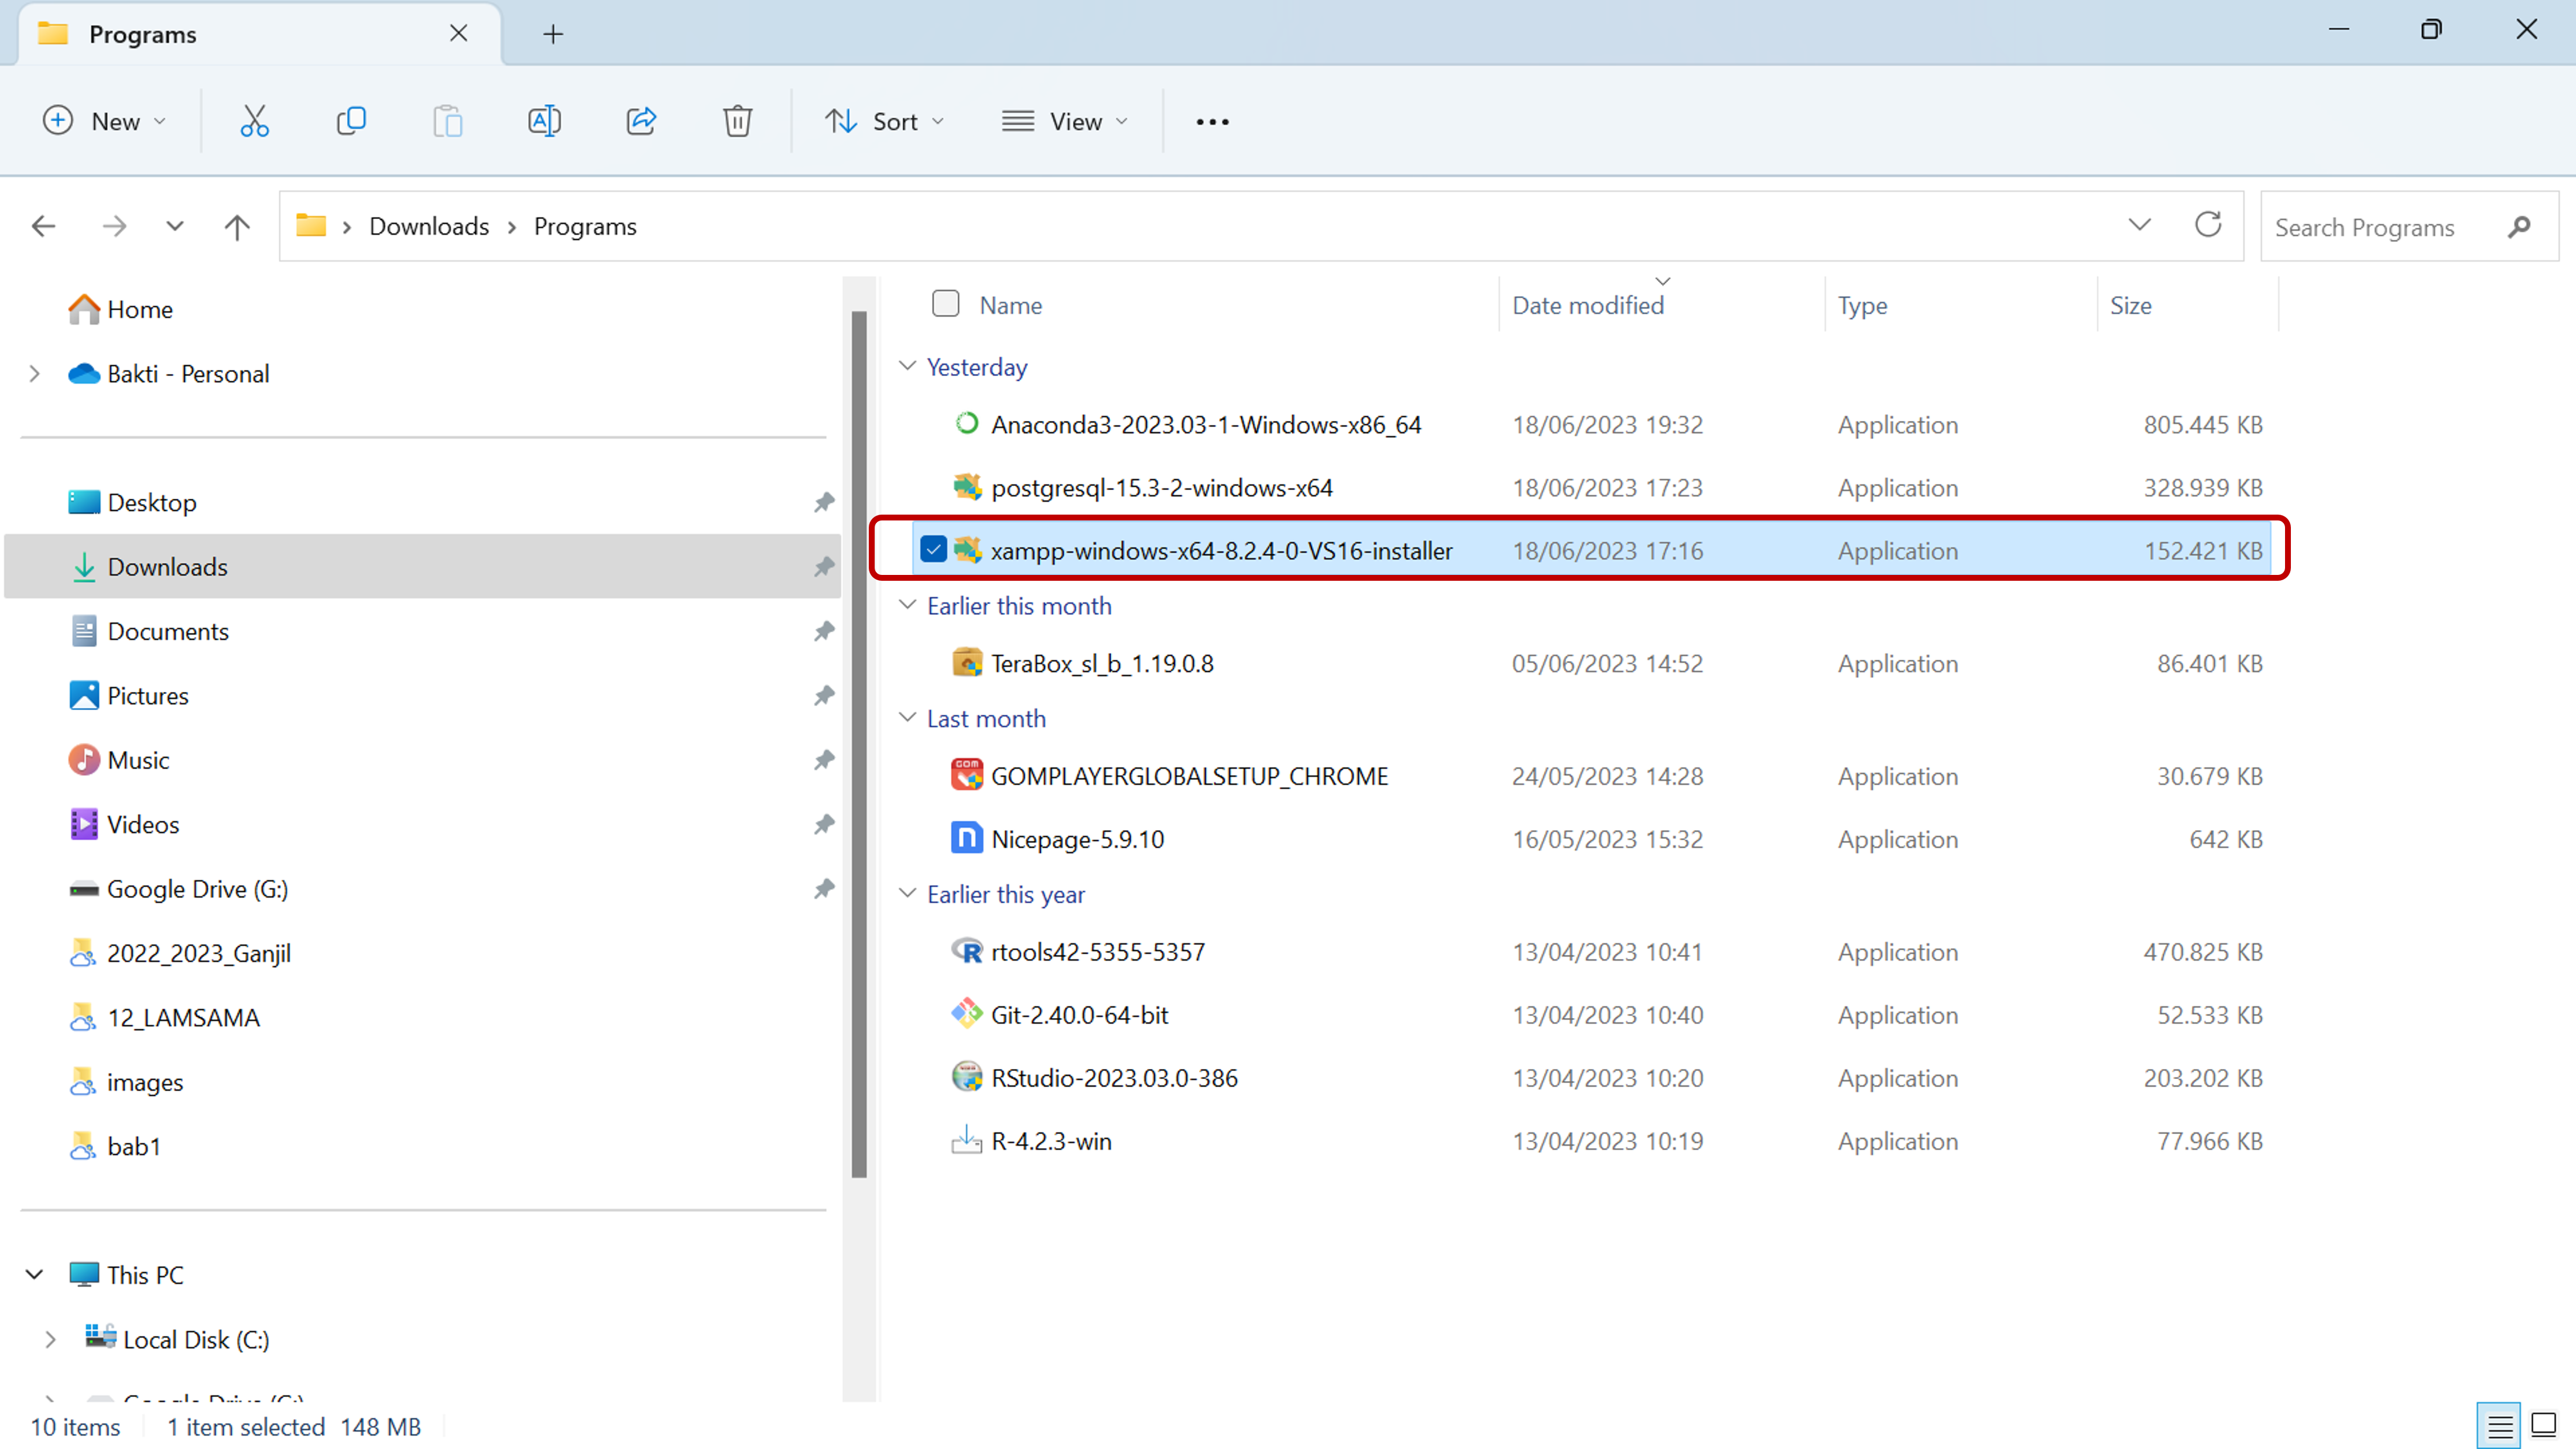
\includegraphics[width=1\linewidth]{./images/Bab1/xampp1} 

}

\caption{Langkah 2, Instalasi XAMPP)}\label{fig:install-xammp}
\end{figure}

Selanjutnya, akan muncul Warning di klik \textbf{OK}

\begin{figure}

{\centering 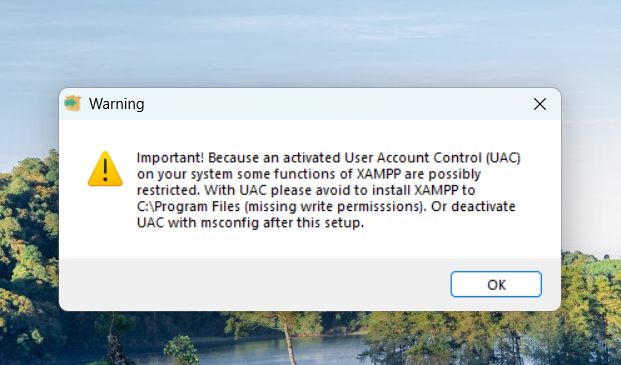
\includegraphics[width=1\linewidth]{./images/Bab1/xampp2} 

}

\caption{Langkah 3, Instalasi XAMPP)}\label{fig:install-xammp2}
\end{figure}

selajutunya klik next

\begin{figure}

{\centering 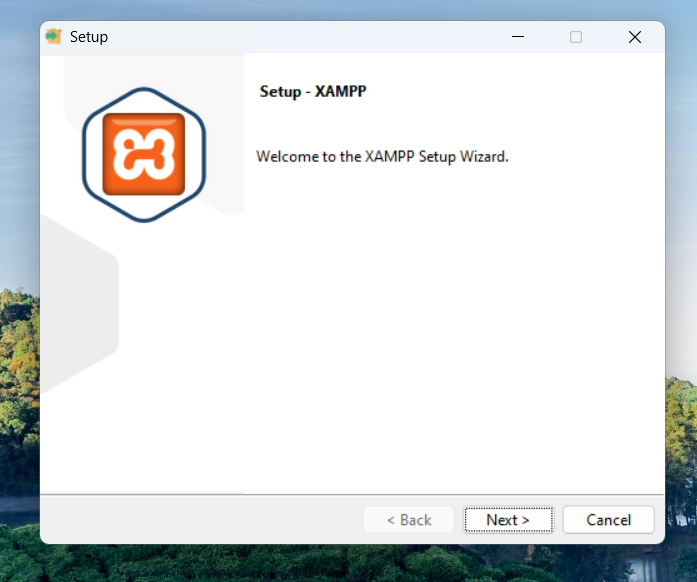
\includegraphics[width=1\linewidth]{./images/Bab1/xampp3} 

}

\caption{Langkah 4: Instalasi XAMPP)}\label{fig:install-xammp3}
\end{figure}

Klik next lagi, karena sudah dipilih secara default oleh XAMPP

\begin{figure}

{\centering 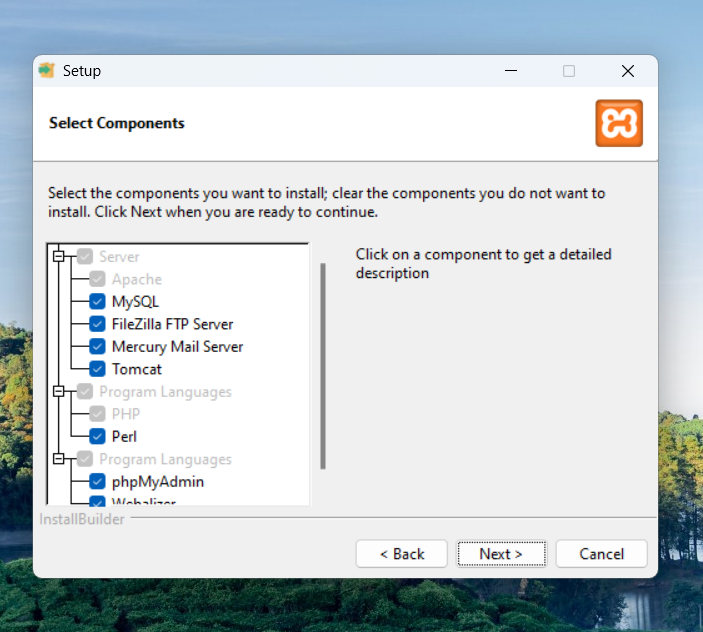
\includegraphics[width=1\linewidth]{./images/Bab1/xampp4} 

}

\caption{Langkah 5, Instalasi XAMPP)}\label{fig:install-xammp4}
\end{figure}

\hypertarget{pilih-folder}{%
\subsection{Pilih Folder}\label{pilih-folder}}

\begin{figure}

{\centering 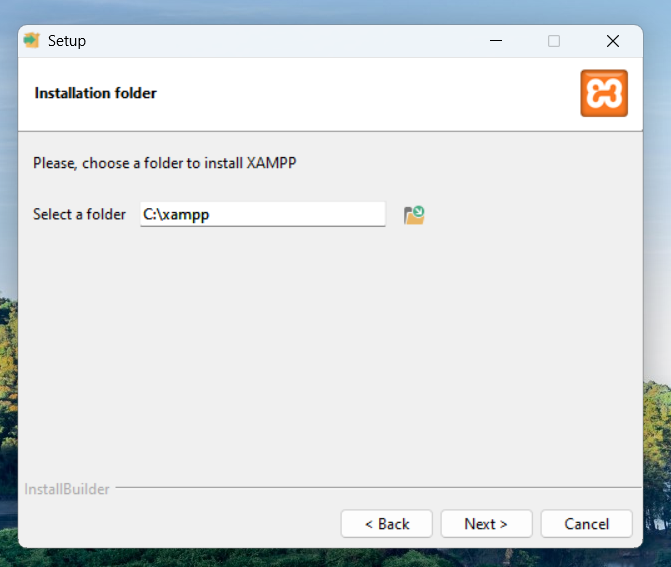
\includegraphics[width=1\linewidth]{./images/Bab1/xampp5} 

}

\caption{Langkah 6, Instalasi XAMPP)}\label{fig:install-xammp5}
\end{figure}

Secara default akan membuat folder baru \textbf{C:\textbackslash xampp}, lalu pilih next.

\textbf{note:} jika anda sudah pernah mendownload aplikasi xampp, perlu di hapus terlebih dahulu file xampp yang lama di file \textbf{C:\textbackslash xampp}

\hypertarget{jalankan-proses-instalasi}{%
\subsection{Jalankan proses Instalasi}\label{jalankan-proses-instalasi}}

\begin{figure}

{\centering 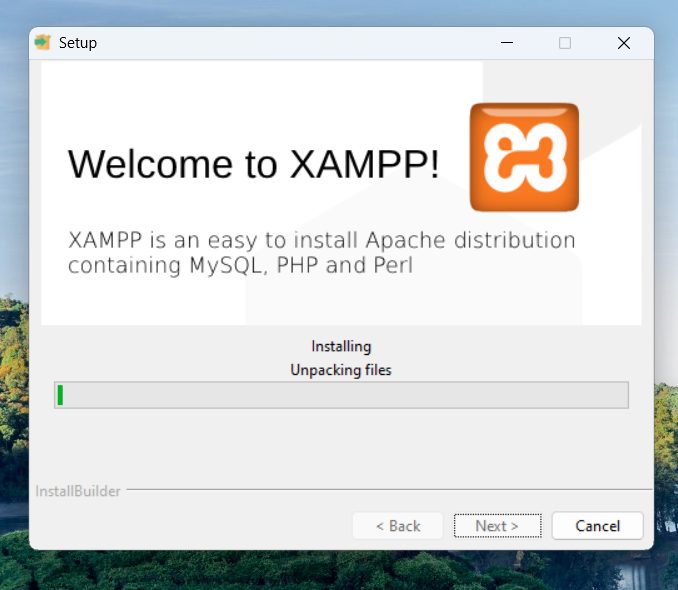
\includegraphics[width=1\linewidth]{./images/Bab1/xampp6} 

}

\caption{Langkah 7, Instalasi XAMPP)}\label{fig:install-xammp6}
\end{figure}

Tunggu proses instalasi selesai \textbf{Biasanya 5-10 menit, tergantung kecepatan komputer anda}.

\hypertarget{xampp-sudah-terinstall}{%
\subsection{XAMPP sudah terinstall}\label{xampp-sudah-terinstall}}

\begin{figure}

{\centering 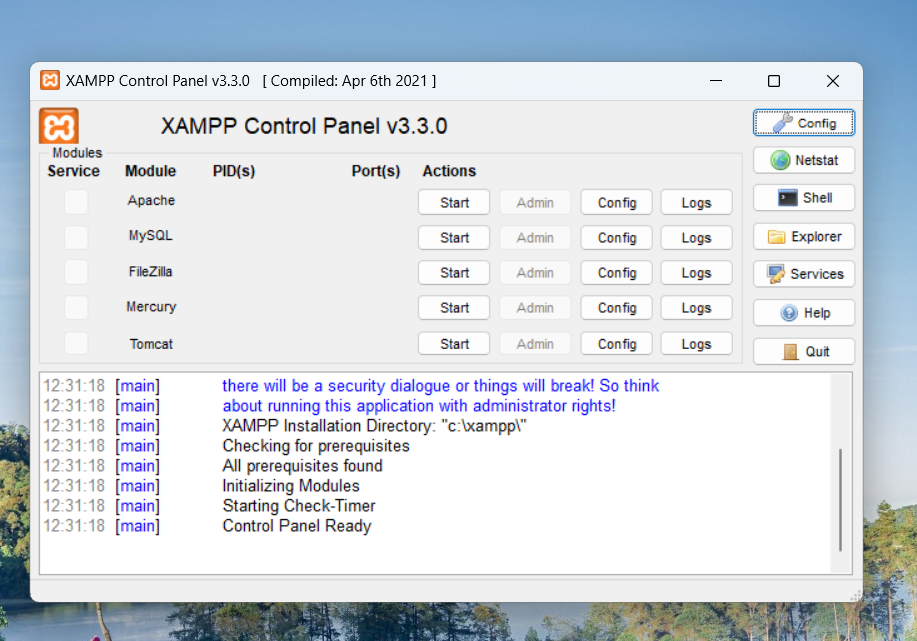
\includegraphics[width=1\linewidth]{./images/Bab1/xampp7} 

}

\caption{Langkah 8, Instalasi XAMPP)}\label{fig:install-xammp7}
\end{figure}

Setelah aplikasi terinstall, sudah bisa digunakan.

\hypertarget{video-instalasi-xampp}{%
\subsection{Video Instalasi XAMPP}\label{video-instalasi-xampp}}

\hypertarget{instalasi-postgresql}{%
\section{Instalasi PostgreSQL}\label{instalasi-postgresql}}

Berikut ini adalah proses langkah demi langkah tentang Cara Menginstal PostgreSQL di Windows:

\hypertarget{buka-browser}{%
\subsection{Buka Browser}\label{buka-browser}}

Klik \url{https://www.postgresql.org/download} and pilih Windows

\begin{figure}

{\centering 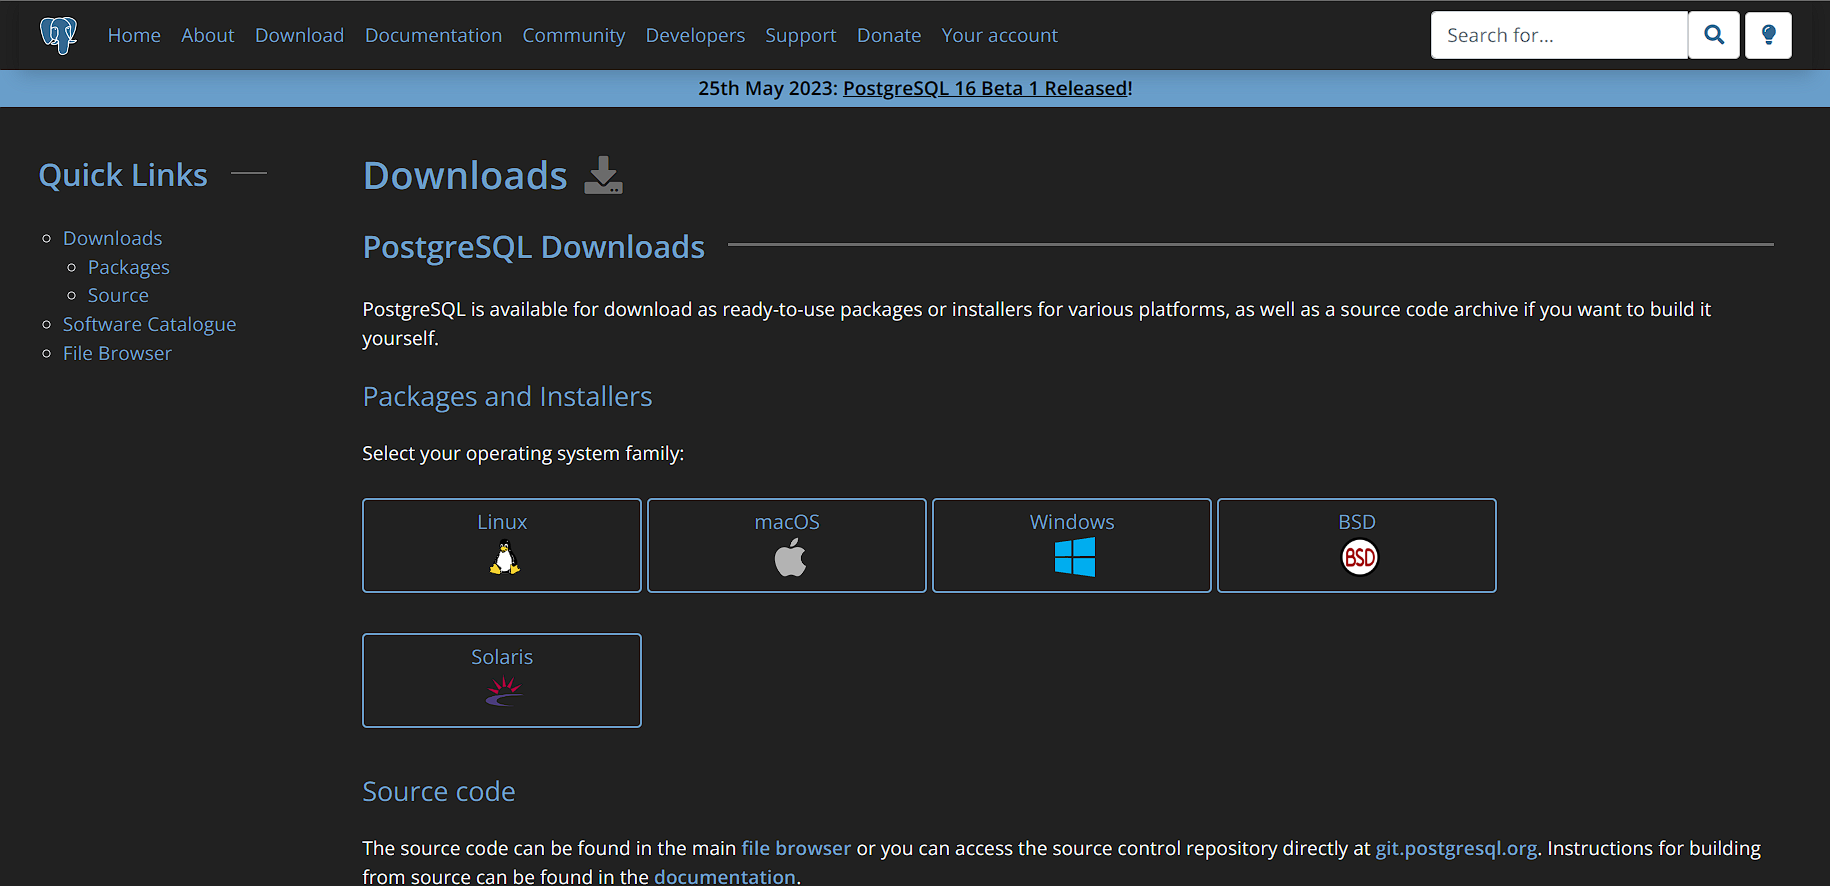
\includegraphics[width=1\linewidth]{./images/Bab1/Postgree0} 

}

\caption{Langkah 1, Instalasi PostgreeSQL)}\label{fig:install-posrgree1}
\end{figure}

\hypertarget{cek-option}{%
\subsection{Cek Option}\label{cek-option}}

Klik Download the installer Interactive Installer by EnterpriseDB

\begin{figure}

{\centering 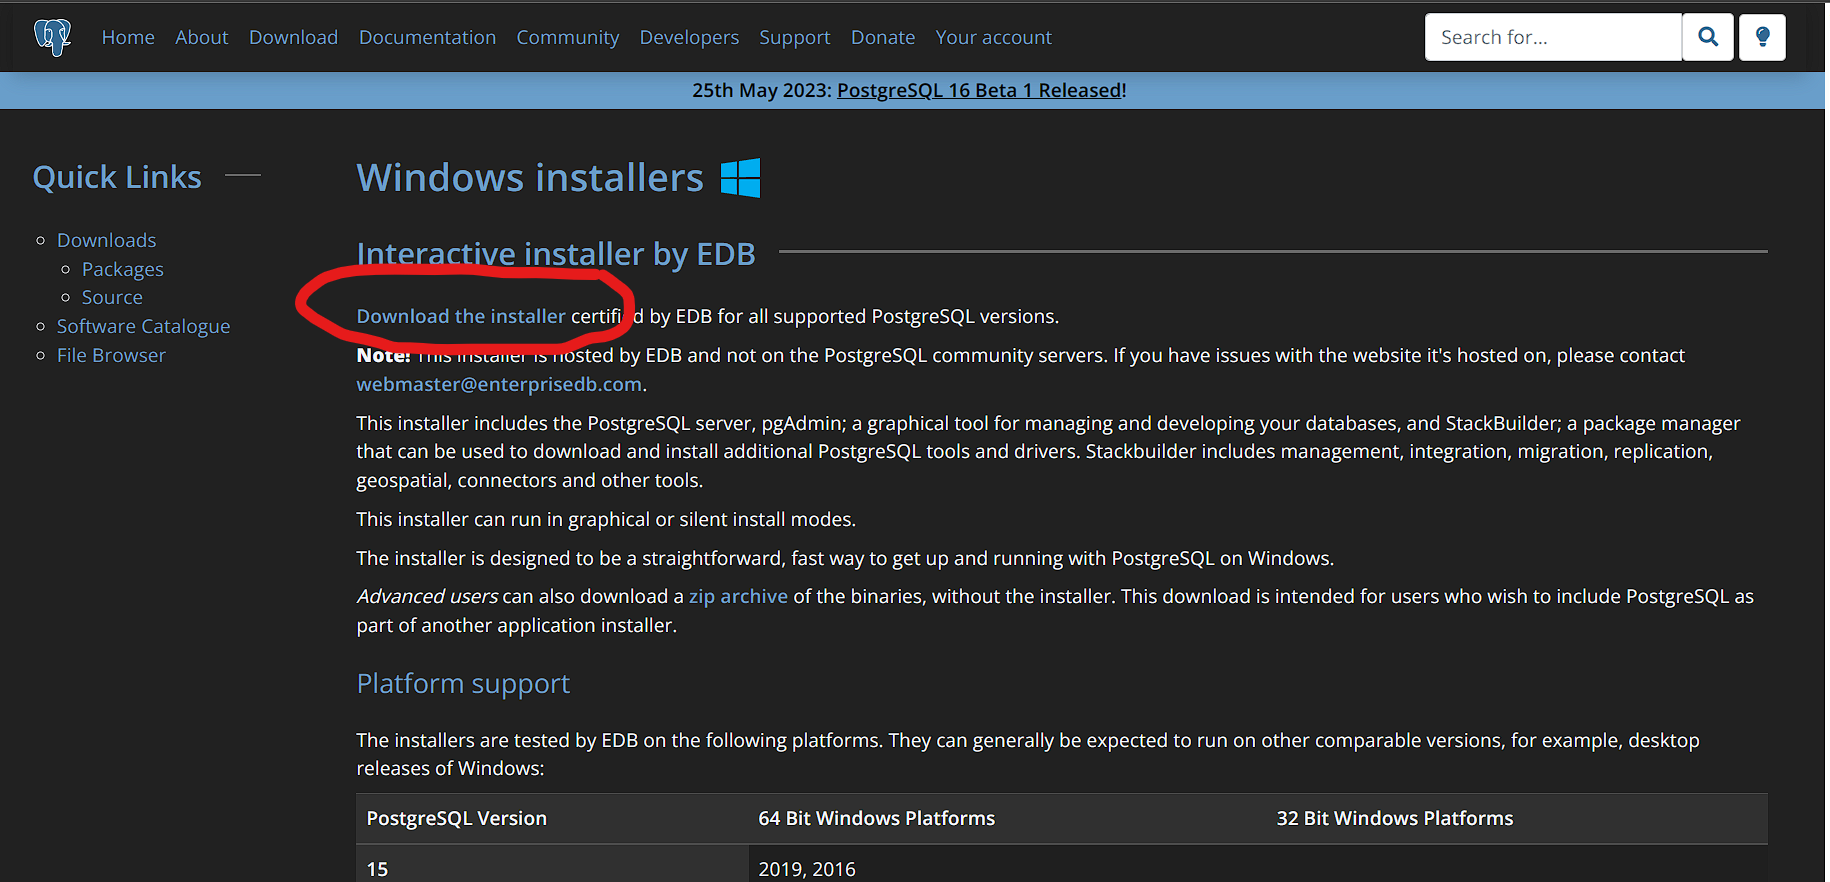
\includegraphics[width=1\linewidth]{./images/Bab1/Postgree1} 

}

\caption{Langkah 2, Instalasi PostgreeSQL)}\label{fig:install-posrgree2}
\end{figure}

\hypertarget{pilih-postgresql-version}{%
\subsection{Pilih PostgreSQL version}\label{pilih-postgresql-version}}

Anda akan diminta untuk memilih versi PostgreSQL dan sistem operasi yang diinginkan. Pilih versi PostgreSQL terbaru dan OS sesuai dengan environment Anda, \textbf{klik tombol download.}

\begin{figure}

{\centering 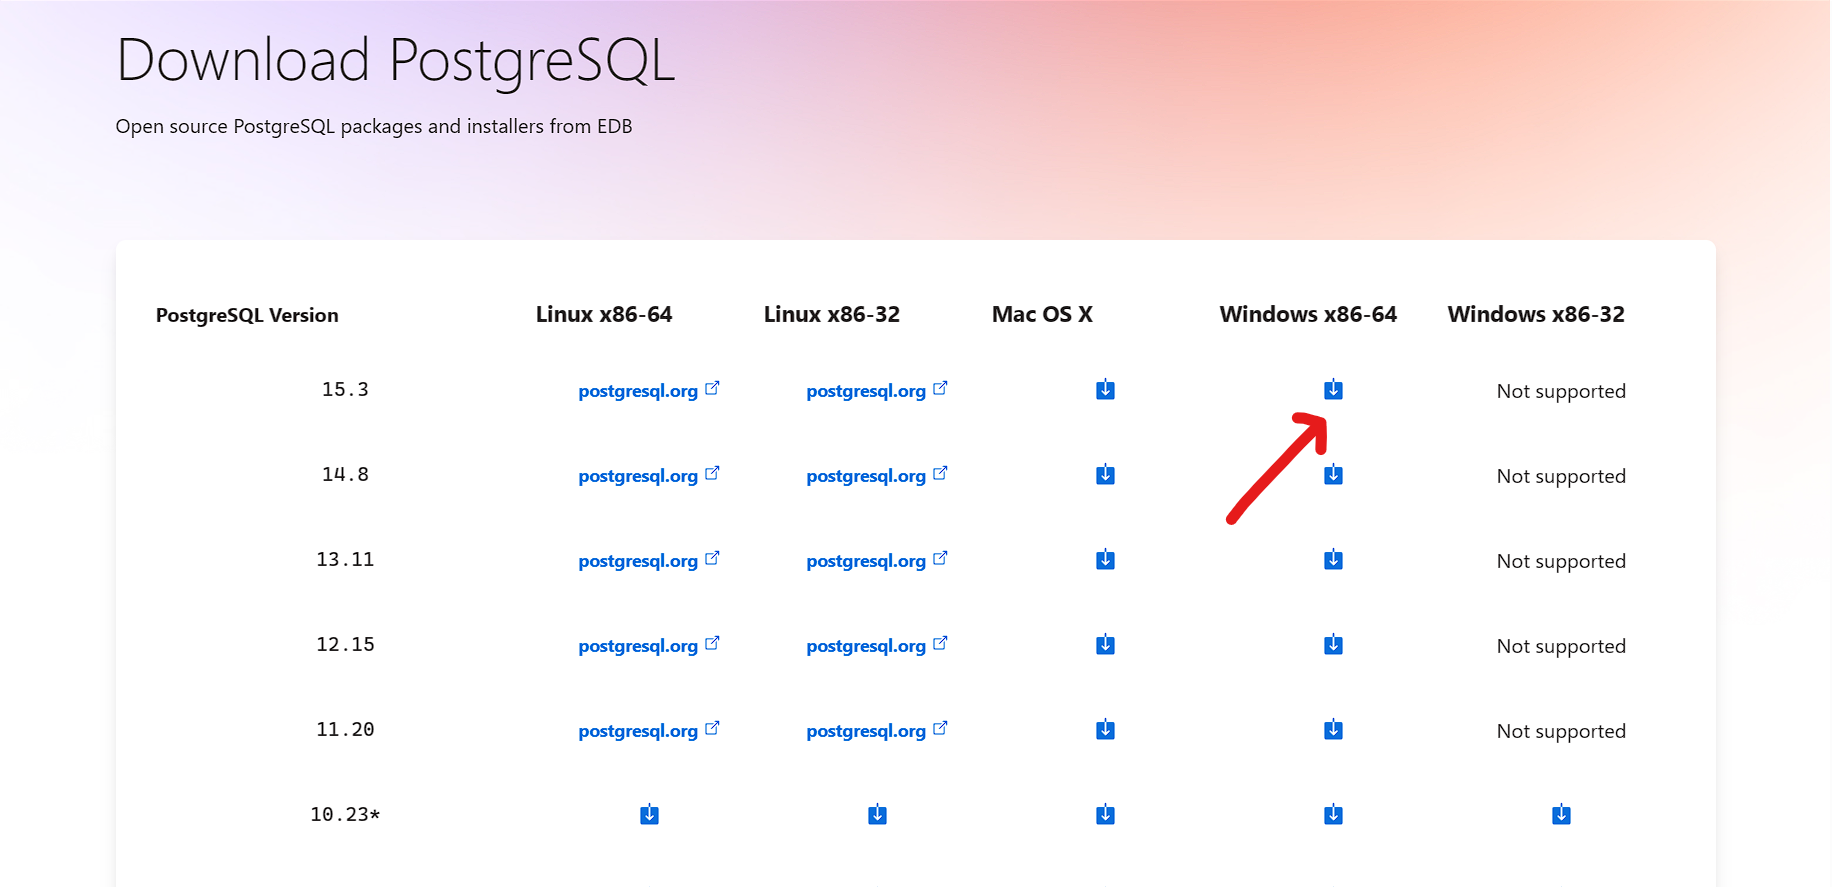
\includegraphics[width=1\linewidth]{./images/Bab1/Postgree2} 

}

\caption{Langkah 3, Instalasi PostgreeSQL)}\label{fig:install-posrgree3}
\end{figure}

\hypertarget{open-exe-file}{%
\subsection{Open exe file}\label{open-exe-file}}

Setelah Anda mengunduh PostgreSQL, buka exe yang telah diunduh dan Klik berikutnya pada layar install welcome screen.

\begin{figure}

{\centering 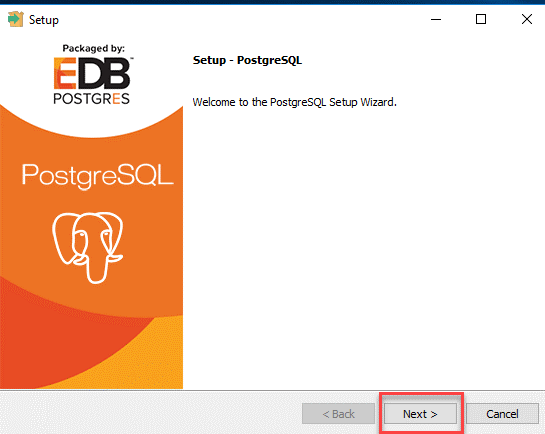
\includegraphics[width=1\linewidth]{./images/Bab1/Postgree3} 

}

\caption{Langkah 4, Instalasi PostgreeSQL)}\label{fig:install-posrgree4}
\end{figure}

\hypertarget{pilih-folder-1}{%
\subsection{Pilih folder}\label{pilih-folder-1}}

Ubah direktori Instalasi jika diperlukan, jika tidak, biarkan default, \textbf{klik Next.}

\begin{figure}

{\centering 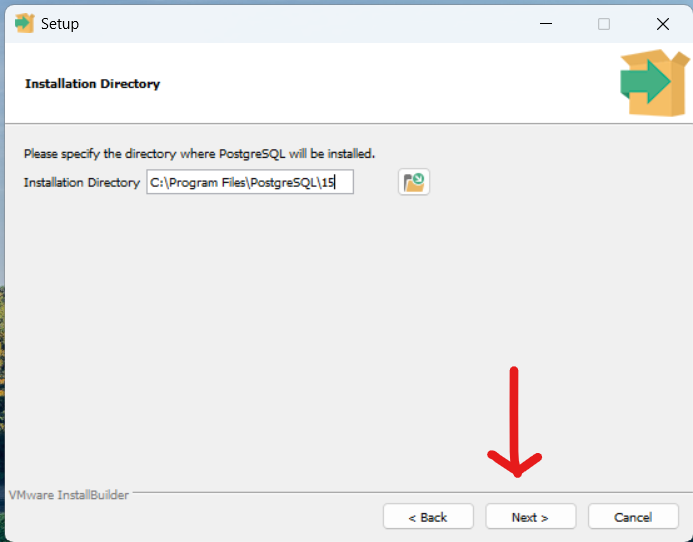
\includegraphics[width=1\linewidth]{./images/Bab1/Postgree4} 

}

\caption{Langkah 5, Instalasi PostgreeSQL)}\label{fig:install-posrgree5}
\end{figure}

\hypertarget{select-components}{%
\subsection{Select components}\label{select-components}}

Anda dapat memilih komponen yang ingin Anda instal di sistem Anda. Anda dapat menghapus centang pada Stack Builder (\emph{disarankan ikuti secara default}), \textbf{klik Next.}

\begin{figure}

{\centering 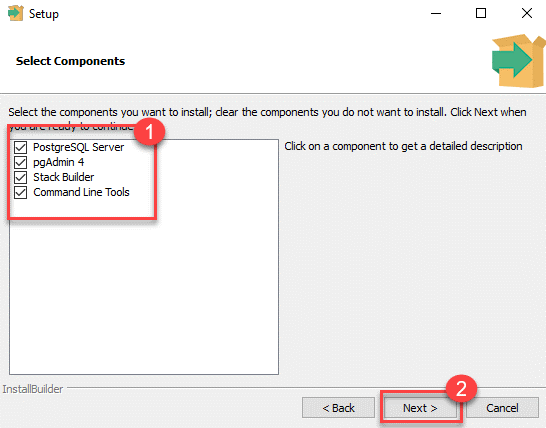
\includegraphics[width=1\linewidth]{./images/Bab1/Postgree5} 

}

\caption{Langkah 6, Instalasi PostgreeSQL)}\label{fig:install-posrgree6}
\end{figure}

\hypertarget{check-data-location}{%
\subsection{Check data location}\label{check-data-location}}

Anda dapat mengubah lokasi data, \textbf{Klik Next.}

\begin{figure}

{\centering 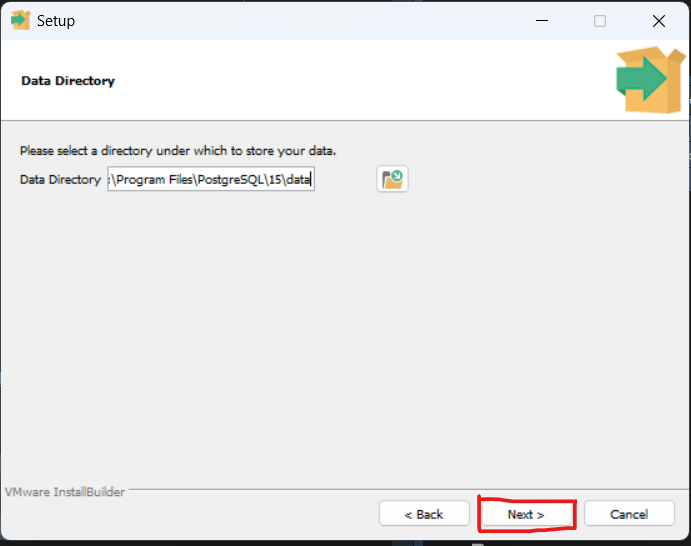
\includegraphics[width=1\linewidth]{./images/Bab1/Postgree6} 

}

\caption{Langkah 7, Instalasi PostgreeSQL)}\label{fig:install-posrgree7}
\end{figure}

\hypertarget{masukan-password}{%
\subsection{Masukan Password}\label{masukan-password}}

Masukkan kata sandi superuser. Catat kata sandi tersebut, \textbf{Klik Next.}

\begin{figure}

{\centering 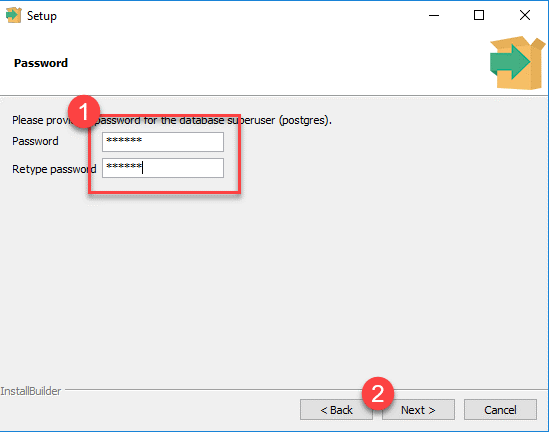
\includegraphics[width=1\linewidth]{./images/Bab1/Postgree7} 

}

\caption{Langkah 8, Instalasi PostgreeSQL)}\label{fig:install-posrgree8}
\end{figure}

\hypertarget{cek-opsi-port}{%
\subsection{Cek opsi port}\label{cek-opsi-port}}

Biarkan nomor port menjadi default, \textbf{Klik Next.}

\begin{figure}

{\centering 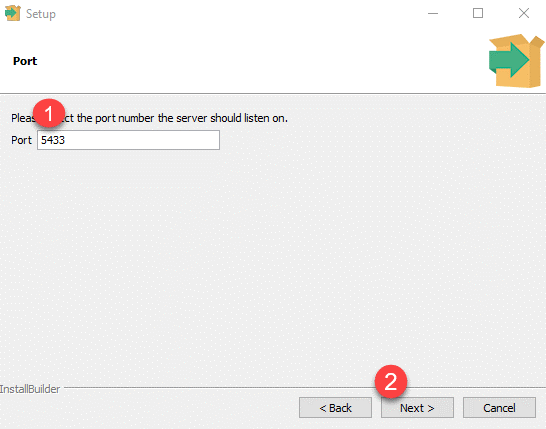
\includegraphics[width=1\linewidth]{./images/Bab1/Postgree8} 

}

\caption{Langkah 9, Instalasi PostgreeSQL)}\label{fig:install-posrgree9}
\end{figure}

\hypertarget{cek-summary}{%
\subsection{Cek Summary}\label{cek-summary}}

Periksa pra-penginstalan summary, \textbf{Klik Next}

\begin{figure}

{\centering 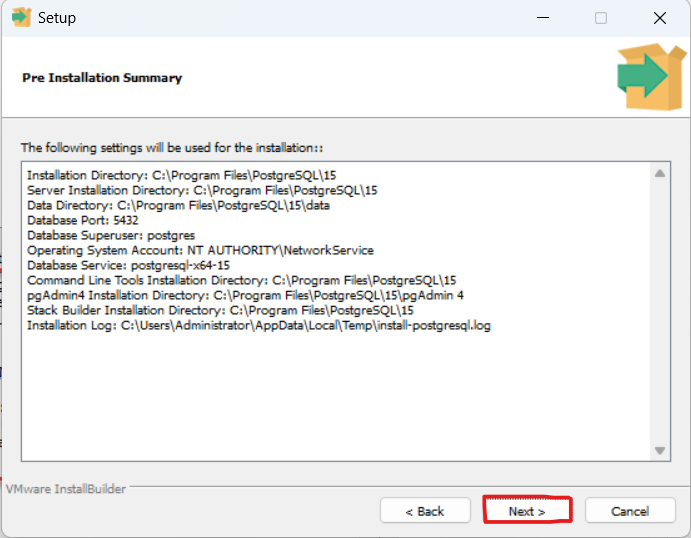
\includegraphics[width=1\linewidth]{./images/Bab1/Postgree9} 

}

\caption{Langkah 10, Instalasi PostgreeSQL)}\label{fig:install-posrgree10}
\end{figure}

\hypertarget{ready-to-install}{%
\subsection{Ready to Install}\label{ready-to-install}}

Klik tombol Next

\begin{figure}

{\centering 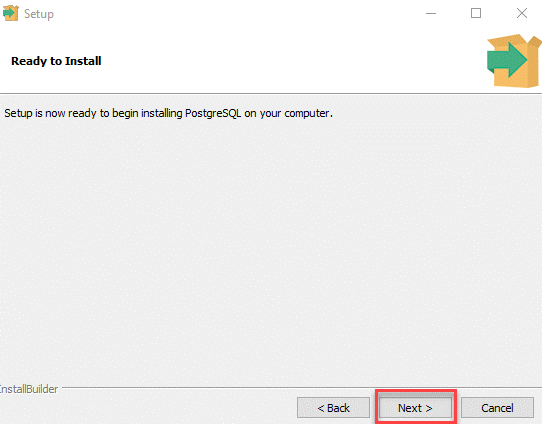
\includegraphics[width=1\linewidth]{./images/Bab1/Postgree10} 

}

\caption{Langkah 11, Instalasi PostgreeSQL)}\label{fig:install-posrgree11}
\end{figure}

\hypertarget{check-stack-builder-prompt}{%
\subsection{Check stack builder prompt}\label{check-stack-builder-prompt}}

Setelah instalasi selesai, Anda akan melihat prompt Stack Builder. Hapus centang pada opsi tersebut. Kita akan menggunakan Stack Builder dalam tutorial selanjutnya, \textbf{Klik Finish.}

\begin{figure}

{\centering 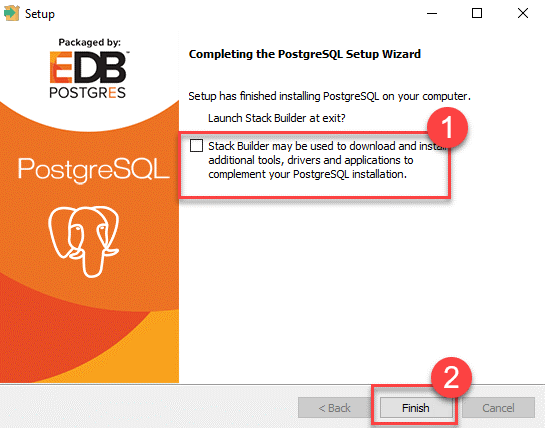
\includegraphics[width=1\linewidth]{./images/Bab1/Postgree11} 

}

\caption{Langkah 12, Instalasi PostgreeSQL)}\label{fig:install-posrgree12}
\end{figure}

\hypertarget{launch-postgresql}{%
\subsection{Launch PostgreSQL}\label{launch-postgresql}}

Untuk launch PostgreSQL, buka Start Menu dan cari pgAdmin 4

\begin{figure}

{\centering 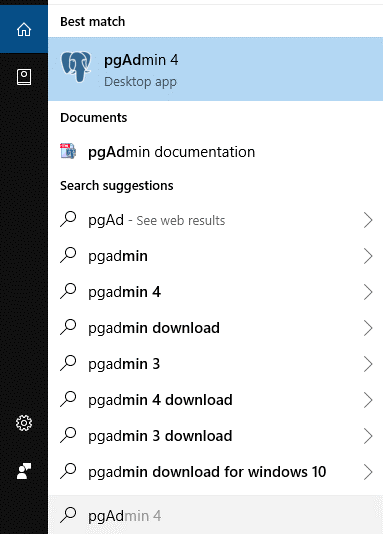
\includegraphics[width=1\linewidth]{./images/Bab1/Postgree12} 

}

\caption{Langkah 13, Instalasi PostgreeSQL)}\label{fig:install-posrgree13}
\end{figure}

\hypertarget{check-pgadmin}{%
\subsection{Check pgAdmin}\label{check-pgadmin}}

Anda akan melihat beranda pgAdmin

\begin{figure}

{\centering 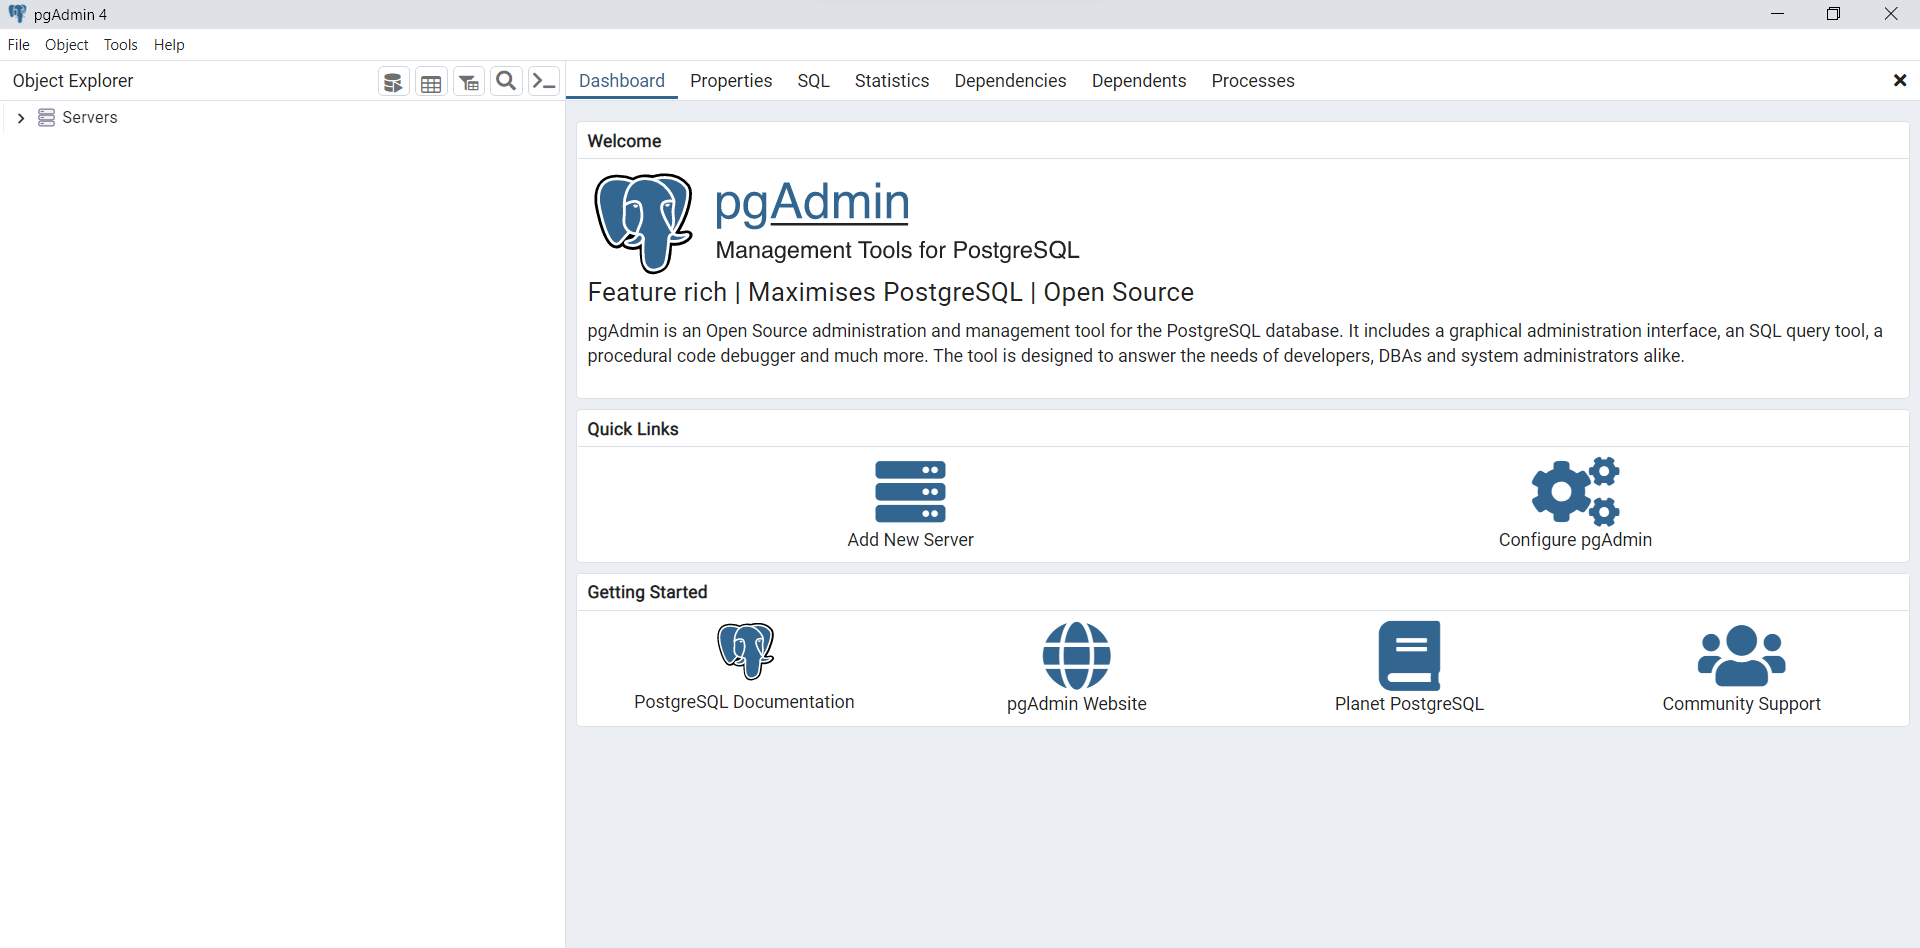
\includegraphics[width=1\linewidth]{./images/Bab1/Postgree13} 

}

\caption{Langkah 14, Instalasi PostgreeSQL)}\label{fig:install-posrgree14}
\end{figure}

\hypertarget{cari-postgresql-15}{%
\subsection{Cari PostgreSQL 15}\label{cari-postgresql-15}}

Klik pada Servers \textgreater{} PostgreSQL 15 di sub sebelah kiri

\begin{figure}

{\centering 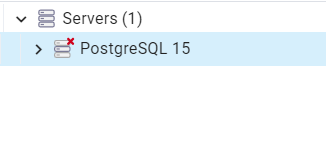
\includegraphics[width=1\linewidth]{./images/Bab1/Postgree14} 

}

\caption{Langkah 15, Instalasi PostgreeSQL)}\label{fig:install-posrgree15}
\end{figure}

\hypertarget{enter-password}{%
\subsection{Enter password}\label{enter-password}}

Masukkan kata sandi superuser yang ditetapkan selama instalasi, \textbf{Klik OK}

\begin{figure}

{\centering 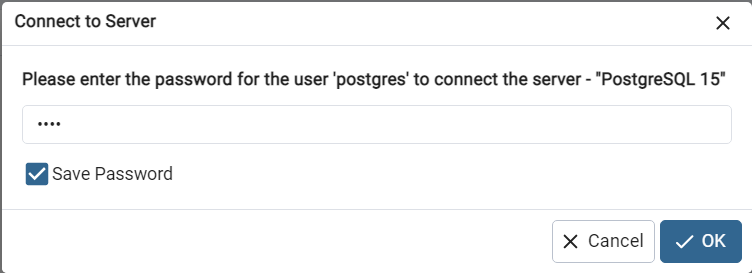
\includegraphics[width=1\linewidth]{./images/Bab1/Postgree15} 

}

\caption{Langkah 16, Instalasi PostgreeSQL)}\label{fig:install-posrgree16}
\end{figure}

\hypertarget{cek-dashboard}{%
\subsection{Cek Dashboard}\label{cek-dashboard}}

Anda akan melihat Dashboard

\begin{figure}

{\centering 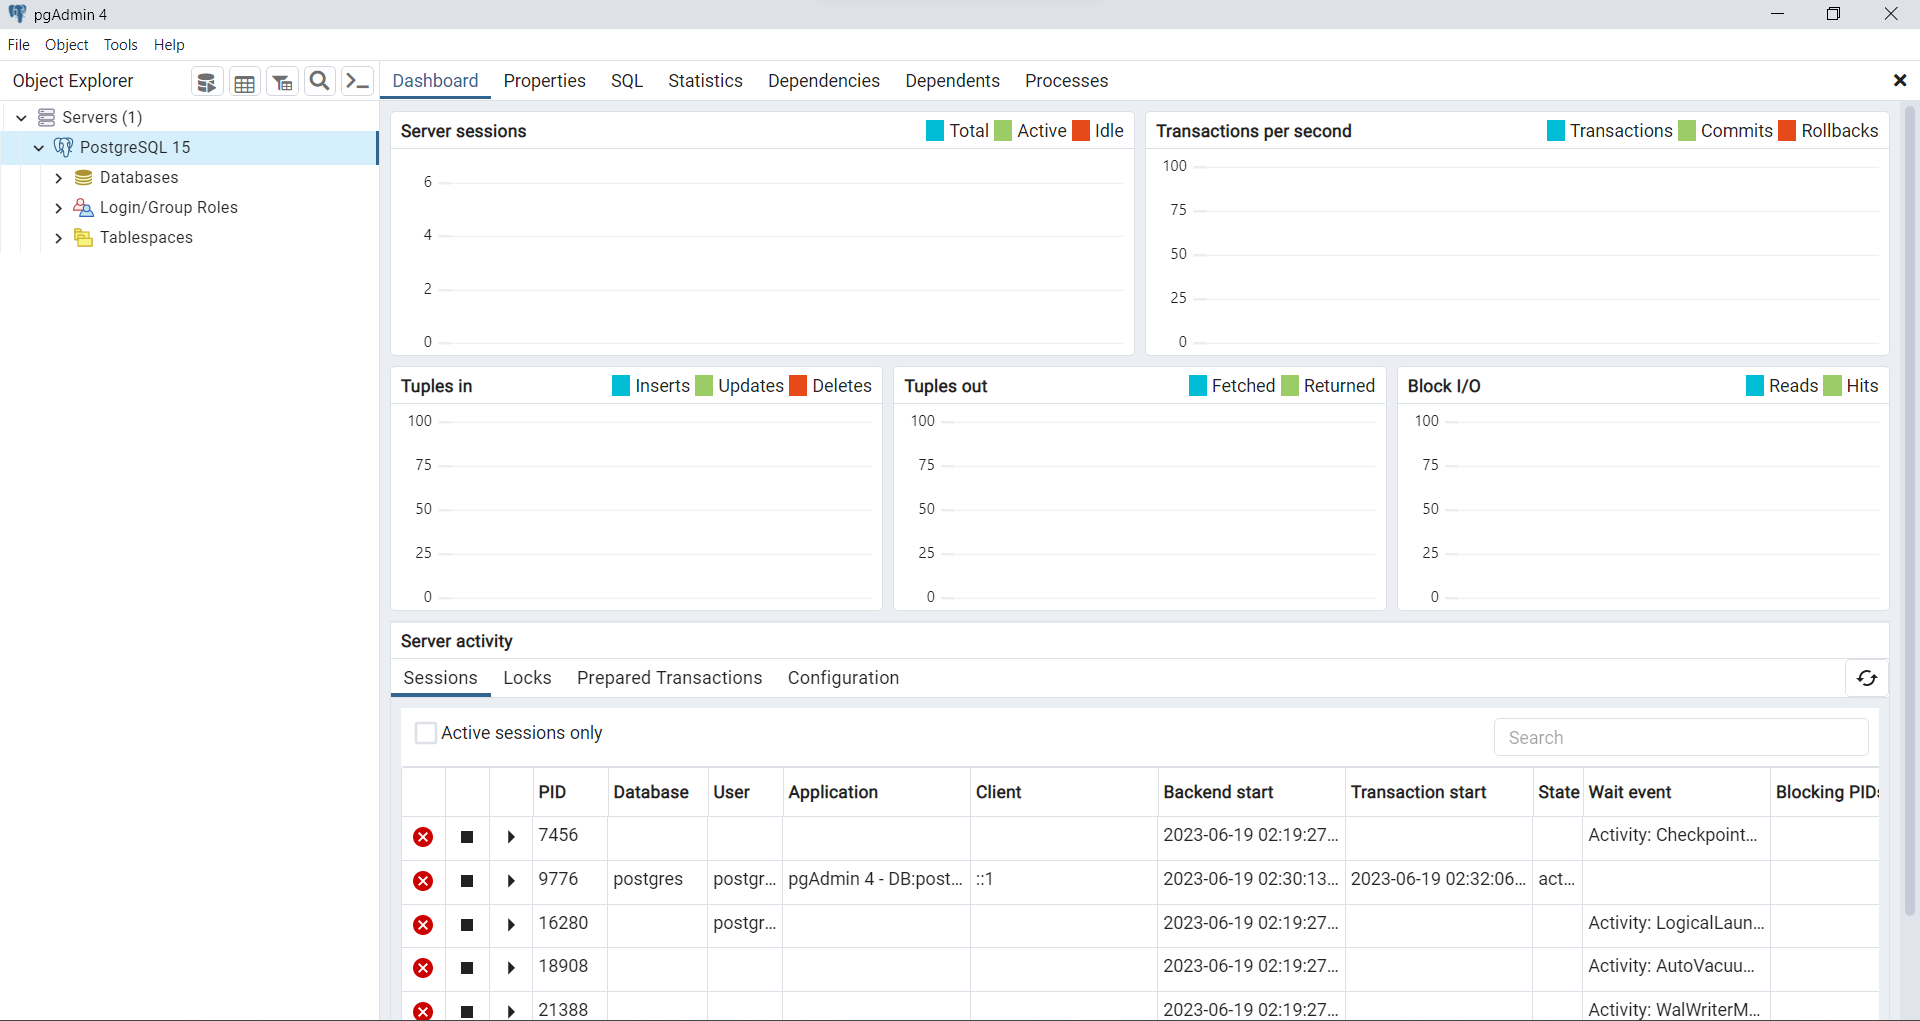
\includegraphics[width=1\linewidth]{./images/Bab1/Postgree16} 

}

\caption{Langkah 17, Instalasi PostgreeSQL)}\label{fig:install-posrgree17}
\end{figure}

\hypertarget{video-instalasi-postgresql}{%
\subsection{Video Instalasi PostgreSQL}\label{video-instalasi-postgresql}}

\hypertarget{praktikum}{%
\section{Praktikum}\label{praktikum}}

\begin{itemize}
\tightlist
\item
  Tutorial di MySQL (CREATE \& Drop Database, Create \& Drop Tabel)
\item
  Tutorial di PostgreeeSQL (CREATE \& Drop Database, Create \& Drop Tabel)
\end{itemize}

\hypertarget{connecting-r-to-sql}{%
\chapter{Connecting R to SQL}\label{connecting-r-to-sql}}

\hypertarget{introduction}{%
\section{Introduction}\label{introduction}}

A database is a structured set of data. Terminology is a little bit different when working with a database management system compared to working with data in R.

\begin{itemize}
\tightlist
\item
  \textbf{field:} variable or quantity
\item
  \textbf{record:} collection of fields
\item
  \textbf{table:} collection of records with all the same fields
\item
  \textbf{database:} collection of tables
\end{itemize}

The relationship between R terminology and database terminology is explained below.

\begin{longtable}[]{@{}ll@{}}
\toprule\noalign{}
R terminology & Database terminology \\
\midrule\noalign{}
\endhead
\bottomrule\noalign{}
\endlastfoot
column & field \\
row & record \\
data frame & table \\
types of columns & table schema \\
collection of data & frames database \\
\end{longtable}

\begin{center}\rule{0.5\linewidth}{0.5pt}\end{center}

\hypertarget{connecting-r-to-sql-1}{%
\section{Connecting R to SQL}\label{connecting-r-to-sql-1}}

Connecting R to SQL databases allows you to leverage the power of R for data analysis while directly interacting with and querying data stored in relational databases. This connection enables you to retrieve, manipulate, and analyze data using SQL queries within your R environment.

\begin{figure}

{\centering 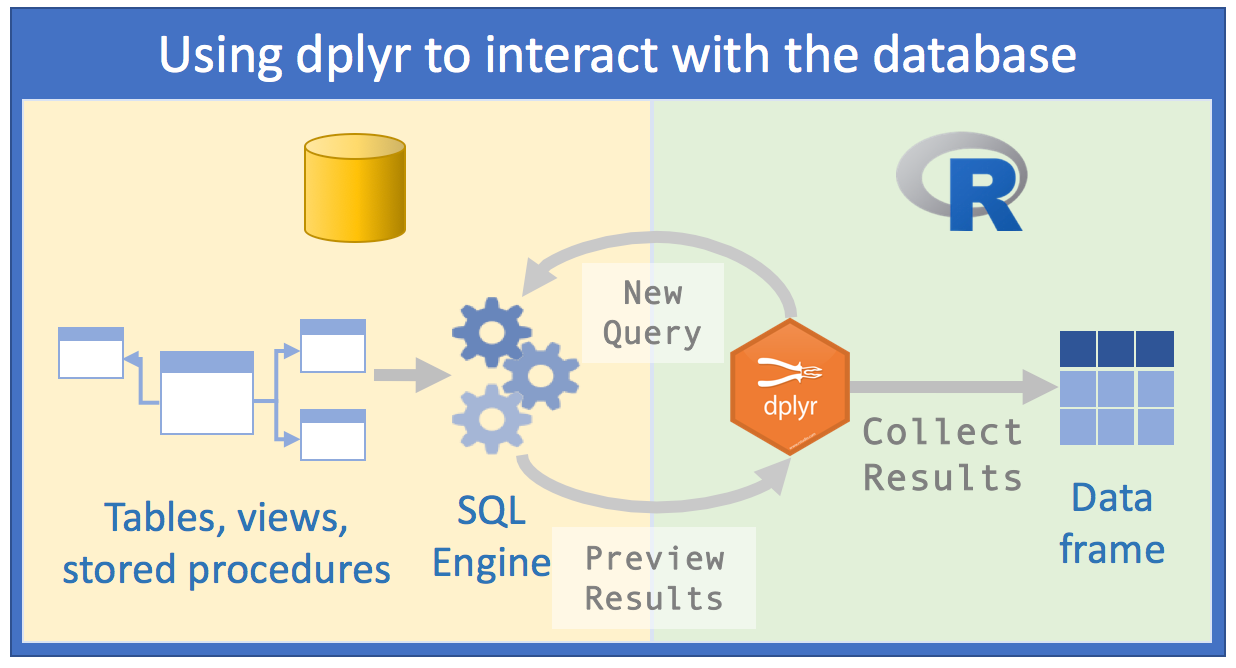
\includegraphics[width=1\linewidth]{./images/Bab2/coneccting_db_in_R} 

}

\caption{Connecting R to SQL [https://rviews.rstudio.com](https://rviews.rstudio.com/2017/05/17/databases-using-r/)}\label{fig:coneccting}
\end{figure}

Here's a step-by-step introduction to connecting R to an SQL database:

\hypertarget{install-required-packages}{%
\subsection{Install Required Packages}\label{install-required-packages}}

First, you need to install R packages that facilitate database connections and SQL interactions. The DBI package provides a common interface for database connections, and you'll also need a database-specific package like RMySQL for MySQL, RPostgreSQL for PostgreSQL, or RODBC for ODBC connections.

You can install these packages using the following commands:

\begin{Shaded}
\begin{Highlighting}[]
\FunctionTok{install.packages}\NormalTok{(}\FunctionTok{c}\NormalTok{(}
                   \StringTok{"RMariaDB"}\NormalTok{,}
                   \StringTok{"RMySQL"}\NormalTok{,}
                   \StringTok{"RPostgres"}
                   \StringTok{"RSQLite"}\NormalTok{,}
\NormalTok{                   )}
\NormalTok{                 )}
\end{Highlighting}
\end{Shaded}

\hypertarget{load-packages}{%
\subsection{Load Packages}\label{load-packages}}

Then, load all these requirement packages:

\begin{Shaded}
\begin{Highlighting}[]
\CommentTok{\# install.packages("pacman")}
\NormalTok{pacman}\SpecialCharTok{::}\FunctionTok{p\_load}\NormalTok{(}
\NormalTok{               RMariaDB,             }\CommentTok{\# Database Interface and \textquotesingle{}MariaDB\textquotesingle{} Driver}
\NormalTok{               RMySQL,               }\CommentTok{\# Database Interface and \textquotesingle{}RMySQL\textquotesingle{} Driver}
\NormalTok{               RPostgres             }\CommentTok{\# Database Interface and \textquotesingle{}RPostgres\textquotesingle{} Driver}
\NormalTok{               RSQLite,              }\CommentTok{\# Database Interface and \textquotesingle{}RSQLite\textquotesingle{} Driver}
\NormalTok{          )}
\end{Highlighting}
\end{Shaded}

\hypertarget{establish-a-connection}{%
\subsection{Establish a Connection}\label{establish-a-connection}}

There are many ways to connect your database with R. This article shows you three of the most common ways:

\hypertarget{mariadb}{%
\subsubsection*{MariaDB}\label{mariadb}}
\addcontentsline{toc}{subsubsection}{MariaDB}

\begin{Shaded}
\begin{Highlighting}[]
\NormalTok{MariaDB }\OtherTok{\textless{}{-}} \FunctionTok{dbConnect}\NormalTok{(RMariaDB}\SpecialCharTok{::}\FunctionTok{MariaDB}\NormalTok{(), }
                  \AttributeTok{user=}\StringTok{\textquotesingle{}root\textquotesingle{}}\NormalTok{,}
                  \AttributeTok{password=}\StringTok{\textquotesingle{}\textquotesingle{}}\NormalTok{, }
                  \AttributeTok{dbname=}\StringTok{\textquotesingle{}bakti\textquotesingle{}}\NormalTok{, }
                  \AttributeTok{host=}\StringTok{\textquotesingle{}localhost\textquotesingle{}}\NormalTok{)}
\FunctionTok{dbListTables}\NormalTok{(MariaDB)                             }\CommentTok{\# table list on your database}
\FunctionTok{dbExecute}\NormalTok{(MariaDB,}\StringTok{"CREATE DATABASE new\_MariaDB"}\NormalTok{)  }\CommentTok{\# Create a new Database}
\FunctionTok{dbExecute}\NormalTok{(MariaDB,}\StringTok{"DROP DATABASE new\_MariaDB"}\NormalTok{)    }\CommentTok{\# Drop a Database}
\end{Highlighting}
\end{Shaded}

\hypertarget{mysql}{%
\subsubsection*{MySQL}\label{mysql}}
\addcontentsline{toc}{subsubsection}{MySQL}

\begin{Shaded}
\begin{Highlighting}[]
\NormalTok{MySQL }\OtherTok{\textless{}{-}} \FunctionTok{dbConnect}\NormalTok{(}\FunctionTok{MySQL}\NormalTok{(), }
                  \AttributeTok{user=}\StringTok{\textquotesingle{}root\textquotesingle{}}\NormalTok{,}
                  \AttributeTok{password=}\StringTok{\textquotesingle{}\textquotesingle{}}\NormalTok{, }
                  \AttributeTok{dbname=}\StringTok{\textquotesingle{}bakti\textquotesingle{}}\NormalTok{, }
                  \AttributeTok{host=}\StringTok{\textquotesingle{}localhost\textquotesingle{}}\NormalTok{)}
\FunctionTok{dbListTables}\NormalTok{(MySQL)                               }\CommentTok{\# table list on your database}
\FunctionTok{dbExecute}\NormalTok{(MySQL,}\StringTok{"CREATE DATABASE new\_MySQL"}\NormalTok{)      }\CommentTok{\# Create a new Database}
\FunctionTok{dbExecute}\NormalTok{(MySQL,}\StringTok{"DROP DATABASE new\_MySQL"}\NormalTok{)        }\CommentTok{\# Drop a Database}
\end{Highlighting}
\end{Shaded}

\hypertarget{postgres}{%
\subsubsection*{Postgres}\label{postgres}}
\addcontentsline{toc}{subsubsection}{Postgres}

\begin{Shaded}
\begin{Highlighting}[]
\NormalTok{postgres }\OtherTok{\textless{}{-}} \FunctionTok{dbConnect}\NormalTok{(RPostgres}\SpecialCharTok{::}\FunctionTok{Postgres}\NormalTok{(), }
                  \AttributeTok{user=}\StringTok{\textquotesingle{}postgres\textquotesingle{}}\NormalTok{,}
                  \AttributeTok{password=}\StringTok{\textquotesingle{}1234\textquotesingle{}}\NormalTok{, }
                  \AttributeTok{dbname=}\StringTok{\textquotesingle{}postgres\textquotesingle{}}\NormalTok{, }
                  \AttributeTok{host=}\StringTok{\textquotesingle{}localhost\textquotesingle{}}\NormalTok{)}
\FunctionTok{dbListTables}\NormalTok{(postgres)                               }\CommentTok{\# table list on your database}
\FunctionTok{dbExecute}\NormalTok{(postgres,}\StringTok{"CREATE DATABASE new\_MySQL"}\NormalTok{)      }\CommentTok{\# Create a new Database}
\FunctionTok{dbExecute}\NormalTok{(postgres,}\StringTok{"DROP DATABASE new\_MySQL"}\NormalTok{)        }\CommentTok{\# Drop a Database}
\end{Highlighting}
\end{Shaded}

\hypertarget{sqlite}{%
\subsubsection*{SQLite}\label{sqlite}}
\addcontentsline{toc}{subsubsection}{SQLite}

\begin{Shaded}
\begin{Highlighting}[]
\NormalTok{RSQLite }\OtherTok{\textless{}{-}} \FunctionTok{dbConnect}\NormalTok{(RSQLite}\SpecialCharTok{::}\FunctionTok{SQLite}\NormalTok{(), }\StringTok{"folder\_db/mydb3.sqlite"}\NormalTok{)}
\FunctionTok{dbListTables}\NormalTok{(RSQLite)                             }\CommentTok{\# table list on your database}
\end{Highlighting}
\end{Shaded}

\begin{itemize}
\tightlist
\item
  \emph{Notes:} RSQLite will store the database you created in your current working directory.
\end{itemize}

\hypertarget{import-data}{%
\section{Import Data}\label{import-data}}

This section can be ignored if the data (table) that you need is already registered in your database. If not, then it is necessary to import data set according to your available files, download it below:

\begin{itemize}
\tightlist
\item
  \href{https://raw.githubusercontent.com/dsciencelabs/dataset/master/Customers.csv}{Customers.csv}
\item
  \href{https://raw.githubusercontent.com/dsciencelabs/dataset/master/Categories.csv}{Categories.csv}
\item
  \href{https://raw.githubusercontent.com/dsciencelabs/dataset/master/Employees.csv}{Employees.csv}
\item
  \href{https://raw.githubusercontent.com/dsciencelabs/dataset/master/OrderDetails.csv}{OrderDetails.csv}\\
\item
  \href{https://raw.githubusercontent.com/dsciencelabs/dataset/master/Orders.csv}{Orders.csv}
\item
  \href{https://raw.githubusercontent.com/dsciencelabs/dataset/master/Products.csv}{Products.csv}
\item
  \href{https://raw.githubusercontent.com/dsciencelabs/dataset/master/Shippers.csv}{Shippers.csv}
\item
  \href{https://raw.githubusercontent.com/dsciencelabs/dataset/master/Suppliers.csv}{Suppliers.csv}
\item
  \href{https://view.officeapps.live.com/op/view.aspx?src=https\%3A\%2F\%2Fraw.githubusercontent.com\%2Fdsciencelabs\%2Fdataset\%2Fmaster\%2FRawDatabase.xlsx\&wdOrigin=BROWSELINK}{RawDatabase.xlsx}
\end{itemize}

\hypertarget{csv-files}{%
\subsection{CSV Files}\label{csv-files}}

When you're working with files in R, such as reading data from a CSV file or saving plots as image files, R needs to know the location of these files. By setting the working directory, you provide a starting point for R to look for and save files.

In R, the setwd() function is used to set the working directory for your R session. The working directory is the folder on your computer where R will look for files and where it will save files unless you specify a different location. Here's why the setwd() function is important and when you might use it:

\begin{Shaded}
\begin{Highlighting}[]
\CommentTok{\# Set the working directory}
\FunctionTok{setwd}\NormalTok{(}\StringTok{"/path/to/your/folder"}\NormalTok{)}
\end{Highlighting}
\end{Shaded}

\begin{Shaded}
\begin{Highlighting}[]
\CommentTok{\# Now you can read CSV files without specifying the full path}
\NormalTok{data }\OtherTok{\textless{}{-}} \FunctionTok{read.csv}\NormalTok{(}\StringTok{"file.csv"}\NormalTok{)}
\end{Highlighting}
\end{Shaded}

Replace ``/path/to/your/folder'' with the actual path to the folder containing your CSV files. Then, you can run the following code!.

\begin{Shaded}
\begin{Highlighting}[]
\NormalTok{Customers   }\OtherTok{\textless{}{-}}\FunctionTok{read.csv}\NormalTok{(}\StringTok{"data/Customers.csv"}\NormalTok{)}
\NormalTok{Categories  }\OtherTok{\textless{}{-}}\FunctionTok{read.csv}\NormalTok{(}\StringTok{"data/Categories.csv"}\NormalTok{)  }
\NormalTok{Employees   }\OtherTok{\textless{}{-}}\FunctionTok{read.csv}\NormalTok{(}\StringTok{"data/Employees.csv"}\NormalTok{)  }
\NormalTok{OrderDetails}\OtherTok{\textless{}{-}}\FunctionTok{read.csv}\NormalTok{(}\StringTok{"data/OrderDetails.csv"}\NormalTok{)  }
\NormalTok{Orders      }\OtherTok{\textless{}{-}}\FunctionTok{read.csv}\NormalTok{(}\StringTok{"data/Orders.csv"}\NormalTok{)  }
\NormalTok{Products    }\OtherTok{\textless{}{-}}\FunctionTok{read.csv}\NormalTok{(}\StringTok{"data/Products.csv"}\NormalTok{)  }
\NormalTok{Shippers    }\OtherTok{\textless{}{-}}\FunctionTok{read.csv}\NormalTok{(}\StringTok{"data/Shippers.csv"}\NormalTok{)}
\NormalTok{Suppliers   }\OtherTok{\textless{}{-}}\FunctionTok{read.csv}\NormalTok{(}\StringTok{"data/Suppliers.csv"}\NormalTok{)  }
\end{Highlighting}
\end{Shaded}

\hypertarget{xlsx-files}{%
\subsection{XLSX Files}\label{xlsx-files}}

\begin{Shaded}
\begin{Highlighting}[]
\FunctionTok{library}\NormalTok{(}\StringTok{"readxl"}\NormalTok{)                                  }
\NormalTok{Customers   }\OtherTok{\textless{}{-}}\FunctionTok{read\_excel}\NormalTok{(}\StringTok{"data/RawDatabase.xlsx"}\NormalTok{,}\AttributeTok{sheet=}\DecValTok{1}\NormalTok{)      }
\NormalTok{Categories  }\OtherTok{\textless{}{-}}\FunctionTok{read\_excel}\NormalTok{(}\StringTok{"data/RawDatabase.xlsx"}\NormalTok{,}\AttributeTok{sheet=}\DecValTok{2}\NormalTok{) }
\NormalTok{Employees   }\OtherTok{\textless{}{-}}\FunctionTok{read\_excel}\NormalTok{(}\StringTok{"data/RawDatabase.xlsx"}\NormalTok{,}\AttributeTok{sheet=}\DecValTok{3}\NormalTok{)}
\NormalTok{OrderDetails}\OtherTok{\textless{}{-}}\FunctionTok{read\_excel}\NormalTok{(}\StringTok{"data/RawDatabase.xlsx"}\NormalTok{,}\AttributeTok{sheet=}\DecValTok{4}\NormalTok{) }
\NormalTok{Orders      }\OtherTok{\textless{}{-}}\FunctionTok{read\_excel}\NormalTok{(}\StringTok{"data/RawDatabase.xlsx"}\NormalTok{,}\AttributeTok{sheet=}\DecValTok{5}\NormalTok{)}
\NormalTok{Products    }\OtherTok{\textless{}{-}}\FunctionTok{read\_excel}\NormalTok{(}\StringTok{"data/RawDatabase.xlsx"}\NormalTok{,}\AttributeTok{sheet=}\DecValTok{6}\NormalTok{) }
\NormalTok{Shippers    }\OtherTok{\textless{}{-}}\FunctionTok{read\_excel}\NormalTok{(}\StringTok{"data/RawDatabase.xlsx"}\NormalTok{,}\AttributeTok{sheet=}\DecValTok{7}\NormalTok{)  }
\NormalTok{Suppliers   }\OtherTok{\textless{}{-}}\FunctionTok{read\_excel}\NormalTok{(}\StringTok{"data/RawDatabase.xlsx"}\NormalTok{,}\AttributeTok{sheet=}\DecValTok{8}\NormalTok{)  }
\end{Highlighting}
\end{Shaded}

\hypertarget{write-dataframe-to-database}{%
\section{Write Dataframe to Database}\label{write-dataframe-to-database}}

The key here is the \texttt{dbWriteTable} function which allows us to write an R data frame directly to a database table. The data frame's column names will be used as the database table's fields. In the following example I use \texttt{RMariaDB} connection, you can apply another driver as you like.

\begin{Shaded}
\begin{Highlighting}[]
\NormalTok{new\_con }\OtherTok{\textless{}{-}} \FunctionTok{dbConnect}\NormalTok{(}\FunctionTok{MariaDB}\NormalTok{(), }
                  \AttributeTok{user=}\StringTok{\textquotesingle{}root\textquotesingle{}}\NormalTok{,}
                  \AttributeTok{password=}\StringTok{\textquotesingle{}\textquotesingle{}}\NormalTok{, }
                  \AttributeTok{dbname=}\StringTok{\textquotesingle{}new\_MariaDB\textquotesingle{}}\NormalTok{, }
                  \AttributeTok{host=}\StringTok{\textquotesingle{}localhost\textquotesingle{}}\NormalTok{)}

\FunctionTok{dbWriteTable}\NormalTok{(new\_con, }\StringTok{"Customers"}\NormalTok{, Customers, }\AttributeTok{append=}\NormalTok{T) }
\FunctionTok{dbWriteTable}\NormalTok{(new\_con, }\StringTok{"Categories"}\NormalTok{, Categories, }\AttributeTok{append=}\NormalTok{T) }
\FunctionTok{dbWriteTable}\NormalTok{(new\_con, }\StringTok{"Employees"}\NormalTok{, Employees, }\AttributeTok{append=}\NormalTok{T) }
\FunctionTok{dbWriteTable}\NormalTok{(new\_con, }\StringTok{"OrderDetails"}\NormalTok{, OrderDetails, }\AttributeTok{append=}\NormalTok{T) }
\FunctionTok{dbWriteTable}\NormalTok{(new\_con, }\StringTok{"Orders"}\NormalTok{, Orders, }\AttributeTok{append=}\NormalTok{T) }
\FunctionTok{dbWriteTable}\NormalTok{(new\_con, }\StringTok{"Products"}\NormalTok{, Products, }\AttributeTok{append=}\NormalTok{T) }
\FunctionTok{dbWriteTable}\NormalTok{(new\_con, }\StringTok{"Shippers"}\NormalTok{, Shippers, }\AttributeTok{append=}\NormalTok{T) }
\FunctionTok{dbWriteTable}\NormalTok{(new\_con, }\StringTok{"Suppliers"}\NormalTok{, Suppliers, }\AttributeTok{append=}\NormalTok{T) }
\end{Highlighting}
\end{Shaded}

\emph{Note:} Some important things that must be considered when storing table data are as follows:

\begin{itemize}
\tightlist
\item
  Data Structure adjustments
\item
  Changes Data type (especially, Date and Time)
\end{itemize}

In this case, we have a problem with the data table \texttt{Employees} and \texttt{Orders}. When you consider these Table (Employees and Orders), you will find there is no date are written correctly in the database. In order to handle this problem, just type the following code in your R console:

\begin{Shaded}
\begin{Highlighting}[]
\FunctionTok{dbRemoveTable}\NormalTok{(new\_con, }\StringTok{"Orders"}\NormalTok{)}
\end{Highlighting}
\end{Shaded}

\begin{Shaded}
\begin{Highlighting}[]
\NormalTok{Orders[}\StringTok{"OrderDate"}\NormalTok{] }\OtherTok{\textless{}{-}}\FunctionTok{as.Date}\NormalTok{(Orders}\SpecialCharTok{$}\NormalTok{OrderDate, }\AttributeTok{format =} \StringTok{"\%Y{-}\%m{-}\%d"}\NormalTok{) }
\end{Highlighting}
\end{Shaded}

\begin{Shaded}
\begin{Highlighting}[]
\FunctionTok{dbWriteTable}\NormalTok{(new\_con, }\StringTok{"Orders"}\NormalTok{, Orders, }\AttributeTok{append=}\NormalTok{T) }
\end{Highlighting}
\end{Shaded}

\emph{Your Exercise:} Do the same thing to update data table \texttt{Employees}

\hypertarget{basic-sql-in-r}{%
\section{Basic SQL in R}\label{basic-sql-in-r}}

\hypertarget{select}{%
\subsection{SELECT}\label{select}}

The SELECT statement is used to select data from a database.

\begin{Shaded}
\begin{Highlighting}[]
\FunctionTok{library}\NormalTok{(DT)}
\NormalTok{df1}\OtherTok{\textless{}{-}}\FunctionTok{dbGetQuery}\NormalTok{(new\_con,}\StringTok{\textquotesingle{}SELECT city}
\StringTok{                         FROM Customers\textquotesingle{}}\NormalTok{)}
\FunctionTok{datatable}\NormalTok{(df1)}
\end{Highlighting}
\end{Shaded}

\hypertarget{where}{%
\subsection{WHERE}\label{where}}

The WHERE clause is used to filter records, extract only those records that fulfill a specified condition.

\begin{Shaded}
\begin{Highlighting}[]
\NormalTok{df2}\OtherTok{\textless{}{-}}\FunctionTok{dbGetQuery}\NormalTok{(new\_con,}\StringTok{"SELECT * }
\StringTok{                         FROM Customers }
\StringTok{                         WHERE Country=\textquotesingle{}Germany\textquotesingle{}"}\NormalTok{)}
\FunctionTok{datatable}\NormalTok{(df2)}
\end{Highlighting}
\end{Shaded}

\hypertarget{insert-into}{%
\subsection{INSERT INTO}\label{insert-into}}

If you are adding values for all the columns of the table, you do not need to specify the column names in the SQL query. However, make sure the order of the values is in the same order as the columns in the table. The INSERT INTO syntax would be as follows:

\begin{Shaded}
\begin{Highlighting}[]
\FunctionTok{dbExecute}\NormalTok{(new\_con,}\StringTok{"INSERT INTO Customers(CustomerName,ContactName,Address,City,PostalCode, Country)}
\StringTok{                   VALUES(\textquotesingle{}Bakti\textquotesingle{},\textquotesingle{}Siregar\textquotesingle{},\textquotesingle{}Jl.Bahagia Selalu\textquotesingle{},\textquotesingle{}Tangerang\textquotesingle{},\textquotesingle{}081369\textquotesingle{},\textquotesingle{}Indonesia\textquotesingle{})"}\NormalTok{)}
\end{Highlighting}
\end{Shaded}

\hypertarget{delete}{%
\subsection{DELETE}\label{delete}}

The DELETE statement is used to delete existing records in a table.

\begin{Shaded}
\begin{Highlighting}[]
\FunctionTok{dbExecute}\NormalTok{(new\_con,}\StringTok{"DELETE FROM Customers}
\StringTok{                   WHERE CustomerName =\textquotesingle{}Bakti\textquotesingle{} "}\NormalTok{)  }
\end{Highlighting}
\end{Shaded}

\hypertarget{update}{%
\subsection{UPDATE}\label{update}}

The UPDATE statement is used to modify the existing records in a table.

\begin{Shaded}
\begin{Highlighting}[]
\FunctionTok{dbExecute}\NormalTok{(new\_con,}\StringTok{"UPDATE Customers}
\StringTok{                   SET ContactName = \textquotesingle{}Alfred Schmidt\textquotesingle{}, City= \textquotesingle{}Frankfurt\textquotesingle{}}
\StringTok{                   WHERE CustomerID = 1"}\NormalTok{)}
\end{Highlighting}
\end{Shaded}

\hypertarget{disconnect-database}{%
\subsection{Disconnect Database}\label{disconnect-database}}

If you are done with the query process and you don't want to use it anymore, you should disconnect the connection from your database.

\begin{Shaded}
\begin{Highlighting}[]
\FunctionTok{dbDisconnect}\NormalTok{(new\_con)                                        }\CommentTok{\# disconnect from your database}
\end{Highlighting}
\end{Shaded}

\hypertarget{your-job}{%
\section{Your Job}\label{your-job}}

\begin{enumerate}
\def\labelenumi{\arabic{enumi}.}
\tightlist
\item
  Write Dataframe to your Database directory, using the following Engine:
\end{enumerate}

\begin{itemize}
\tightlist
\item
  RMySQL
\item
  RPostgres\\
\item
  RSQLite
\end{itemize}

\begin{enumerate}
\def\labelenumi{\arabic{enumi}.}
\setcounter{enumi}{1}
\tightlist
\item
  Create a `Basic Queries' tutorial using all engine that you already use at task no 1, (Such as: \texttt{SELECT}, \texttt{WHERE}, \texttt{INSERT\ INTO}, \texttt{DELETE}, and \texttt{UPDATE})!
\end{enumerate}

\hypertarget{fundamental-sql-in-r}{%
\chapter{Fundamental SQL in R}\label{fundamental-sql-in-r}}

In the previous section, we learned how to connect R to a Database System (SQL) Such as RMariaDB, RMySQL, and RSQLite. In this section, we continue to cover all that you have to know about fundamental operations in SQL (Here, focus on RMySQL).

\hypertarget{connecting-r-to-mysql}{%
\section{Connecting R to MySQL}\label{connecting-r-to-mysql}}

Connecting R to MySQL is made very easy with the \texttt{RMySQL} package. To connect to a MySQL database simply install the package and load the library.

\begin{Shaded}
\begin{Highlighting}[]
\FunctionTok{library}\NormalTok{(RMySQL)}
\NormalTok{MySQL }\OtherTok{\textless{}{-}} \FunctionTok{dbConnect}\NormalTok{(}\FunctionTok{MySQL}\NormalTok{(), }
                  \AttributeTok{user=}\StringTok{\textquotesingle{}root\textquotesingle{}}\NormalTok{,}
                  \AttributeTok{password=}\StringTok{\textquotesingle{}\textquotesingle{}}\NormalTok{, }
                  \AttributeTok{dbname=}\StringTok{\textquotesingle{}mysql\textquotesingle{}}\NormalTok{, }
                  \AttributeTok{host=}\StringTok{\textquotesingle{}localhost\textquotesingle{}}\NormalTok{)}
\FunctionTok{dbListTables}\NormalTok{(MySQL)                  }\CommentTok{\# a list of the tables in our connection}
\end{Highlighting}
\end{Shaded}

\emph{Note:} Open and your XAMPP, click start on Apache and MySQL. Then, make sure you have the admin privilege before creating any database.

\hypertarget{create-db}{%
\section{Create DB}\label{create-db}}

If you want to create a new database, then the CREATE DATABASE statement would be as shown below:

\begin{Shaded}
\begin{Highlighting}[]
\FunctionTok{dbExecute}\NormalTok{(MySQL, }\StringTok{"CREATE DATABASE factory\_db"}\NormalTok{)}
\end{Highlighting}
\end{Shaded}

The result show us \texttt{1}, means that you have succeeded to create a database.

\hypertarget{drop-db}{%
\section{Drop DB}\label{drop-db}}

If you want to delete an existing database, then the DROP DATABASE statement would be as shown below:

\begin{Shaded}
\begin{Highlighting}[]
\FunctionTok{dbExecute}\NormalTok{(MySQL, }\StringTok{"DROP DATABASE factory\_db"}\NormalTok{)}
\end{Highlighting}
\end{Shaded}

The result show us \texttt{0}, means that you have succeeded to remove (Drop) a database.

\hypertarget{create-table}{%
\section{Create Table}\label{create-table}}

Once you have a database, you can continue to create table as shown below:

\begin{Shaded}
\begin{Highlighting}[]
\FunctionTok{dbExecute}\NormalTok{(MySQL, }\StringTok{"CREATE TABLE Persons(}
\StringTok{                 PersonID int,}
\StringTok{                 LastName varchar(255),}
\StringTok{                 FirstName varchar(255),}
\StringTok{                 Address varchar(255),}
\StringTok{                 City varchar(255))"}\NormalTok{)}
\end{Highlighting}
\end{Shaded}

\hypertarget{insert-value}{%
\section{Insert Value}\label{insert-value}}

If you are adding values for all the columns of the table, you do not need to specify the column names in the SQL query. However, make sure the order of the values is in the same order as the columns in the table. The INSERT INTO syntax would be as follows:

\begin{Shaded}
\begin{Highlighting}[]
\FunctionTok{dbExecute}\NormalTok{(MySQL,}\StringTok{"INSERT INTO Persons(PersonID,LastName,FirstName, Address,City)}
\StringTok{                 VALUES(1,\textquotesingle{}Siregar\textquotesingle{},\textquotesingle{}Bakti\textquotesingle{}, \textquotesingle{}Jl.Bahagia\textquotesingle{},\textquotesingle{}Tangerang\textquotesingle{})"}\NormalTok{)}
\end{Highlighting}
\end{Shaded}

\hypertarget{truncate-table}{%
\section{Truncate Table}\label{truncate-table}}

The TRUNCATE TABLE statement is used to delete the data inside a table, but not the table itself.

\begin{Shaded}
\begin{Highlighting}[]
\FunctionTok{dbExecute}\NormalTok{(MySQL, }\StringTok{"TRUNCATE TABLE Persons"}\NormalTok{)}
\end{Highlighting}
\end{Shaded}

\hypertarget{drop-table}{%
\section{Drop Table}\label{drop-table}}

The DROP TABLE statement is used to drop an existing table in a database.

\begin{Shaded}
\begin{Highlighting}[]
\FunctionTok{dbExecute}\NormalTok{(MySQL, }\StringTok{"DROP TABLE Persons"}\NormalTok{)}
\end{Highlighting}
\end{Shaded}

\begin{center}\rule{0.5\linewidth}{0.5pt}\end{center}

\hypertarget{write-table}{%
\section{Write Table}\label{write-table}}

The key here is the \texttt{dbWriteTable} function which allows us to write an R data frame directly to a database table. The data frame's column names will be used as the database table's fields.

\begin{Shaded}
\begin{Highlighting}[]
\NormalTok{Orders      }\OtherTok{\textless{}{-}}\FunctionTok{read.csv}\NormalTok{(}\StringTok{"data/Orders.csv"}\NormalTok{)  }
\FunctionTok{dbWriteTable}\NormalTok{(MySQL, }\StringTok{"Orders"}\NormalTok{, Orders, }\AttributeTok{append=}\NormalTok{T) }
\end{Highlighting}
\end{Shaded}

\hypertarget{alter-table}{%
\section{Alter Table}\label{alter-table}}

The ALTER TABLE statement is used to add, delete, or modify columns in an existing table. The ALTER TABLE statement is also used to add and drop various constraints on an existing table.

\hypertarget{add-column}{%
\section{Add Column}\label{add-column}}

To add a column in a table, use the following syntax:

\begin{Shaded}
\begin{Highlighting}[]
\FunctionTok{dbExecute}\NormalTok{(MySQL, }\StringTok{"ALTER TABLE Orders}
\StringTok{                 ADD Email varchar(255)"}\NormalTok{)}
\end{Highlighting}
\end{Shaded}

\hypertarget{drop-column}{%
\section{Drop Column}\label{drop-column}}

To delete a column in a table, use the following syntax (notice that some database systems don't allow deleting a column):

\begin{Shaded}
\begin{Highlighting}[]
\FunctionTok{dbSendQuery}\NormalTok{(MySQL, }\StringTok{"ALTER TABLE Orders}
\StringTok{                   DROP COLUMN Email"}\NormalTok{)}
\end{Highlighting}
\end{Shaded}

\hypertarget{modify-column}{%
\section{Modify Column}\label{modify-column}}

\begin{Shaded}
\begin{Highlighting}[]
\FunctionTok{dbSendQuery}\NormalTok{(MySQL,}\StringTok{" ALTER TABLE Orders}
\StringTok{                  MODIFY COLUMN OrderDate date"}\NormalTok{)}
\end{Highlighting}
\end{Shaded}

\hypertarget{constraints}{%
\section{Constraints}\label{constraints}}

SQL constraints are used to specify rules for the data in a table. Constraints are used to limit the type of data that can go into a table. This ensures the accuracy and reliability of the data in the table. If there is any violation between the constraint and the data action, the action is aborted.

Constraints can be column level or table level. Column level constraints apply to a column, and table level constraints apply to the whole table. The following constraints are commonly used in SQL:

\begin{itemize}
\tightlist
\item
  \emph{NOT NULL:} Ensures that a column cannot have a NULL value
\item
  \emph{UNIQUE:} Ensures that all values in a column are different
\item
  \emph{PRIMARY KEY:} A combination of a NOT NULL and UNIQUE. Uniquely identifies each row in a table
\item
  \emph{FOREIGN KEY:} Uniquely identifies a row/record in another table
\item
  \emph{CHECK:} Ensures that all values in a column satisfies a specific condition
\item
  \emph{DEFAULT:} Sets a default value for a column when no value is specified
\item
  \emph{INDEX:} Used to create and retrieve data from the database very quickly
\end{itemize}

\hypertarget{not-null}{%
\subsection{Not Null}\label{not-null}}

The following SQL ensures that the ``ID'', ``LastName'', and ``FirstName'' columns will NOT accept NULL values when the ``Persons\_NotNull'' table is created:

\begin{Shaded}
\begin{Highlighting}[]
\FunctionTok{dbSendQuery}\NormalTok{(MySQL,}\StringTok{"CREATE TABLE Person\_NotNull (}
\StringTok{                   ID int NOT NULL,}
\StringTok{                   LastName varchar(255) NOT NULL,}
\StringTok{                   FirstName varchar(255) NOT NULL,}
\StringTok{                   Age int)"}\NormalTok{)}
\end{Highlighting}
\end{Shaded}

\hypertarget{unique}{%
\subsection{Unique}\label{unique}}

The following SQL creates a UNIQUE constraint on the ``ID'' column when the ``Persons'' table is created:

\begin{Shaded}
\begin{Highlighting}[]
\FunctionTok{dbSendQuery}\NormalTok{(MySQL,}\StringTok{"CREATE TABLE Persons\_Unique (ID int NOT NULL UNIQUE,}
\StringTok{                   LastName varchar(255) NOT NULL,}
\StringTok{                   FirstName varchar(255) NOT NULL,}
\StringTok{                   Age int)"}\NormalTok{)}
\end{Highlighting}
\end{Shaded}

To create a UNIQUE constraint on the ``ID'' column when the table is already created, use the following SQL:

\begin{Shaded}
\begin{Highlighting}[]
\FunctionTok{dbSendQuery}\NormalTok{(MySQL,}\StringTok{"ALTER TABLE Persons\_Unique}
\StringTok{                   ADD UNIQUE (ID)"}\NormalTok{)}
\end{Highlighting}
\end{Shaded}

To define a UNIQUE constraint on multiple columns, use the following SQL syntax:

\begin{Shaded}
\begin{Highlighting}[]
\FunctionTok{dbSendQuery}\NormalTok{(MySQL,}\StringTok{"ALTER TABLE Persons\_Unique}
\StringTok{                  ADD CONSTRAINT UNIQUE (ID,LastName)"}
\end{Highlighting}
\end{Shaded}

To drop a UNIQUE constraint, use the following SQL:

\begin{Shaded}
\begin{Highlighting}[]
\FunctionTok{dbSendQuery}\NormalTok{(MySQL,}\StringTok{"ALTER TABLE Persons\_Unique}
\StringTok{                  DROP INDEX ID"}\NormalTok{)}
\end{Highlighting}
\end{Shaded}

\hypertarget{primary-key}{%
\subsection{Primary Key}\label{primary-key}}

The PRIMARY KEY constraint uniquely identifies each record in a table. Primary keys must contain UNIQUE values, and cannot contain NULL values. A table can have only ONE primary key; and in the table, this primary key can consist of single or multiple columns (fields).

\begin{Shaded}
\begin{Highlighting}[]
\FunctionTok{dbSendQuery}\NormalTok{(MySQL,}\StringTok{"CREATE TABLE Persons\_PK (ID int NOT NULL PRIMARY KEY,}
\StringTok{                   LastName varchar(255) NOT NULL,}
\StringTok{                   FirstName varchar(255),}
\StringTok{                   Age int)"}\NormalTok{)}
\end{Highlighting}
\end{Shaded}

To allow naming of a PRIMARY KEY constraint, and for defining a PRIMARY KEY constraint on multiple columns, use the following SQL syntax:

\begin{Shaded}
\begin{Highlighting}[]
\FunctionTok{dbSendQuery}\NormalTok{(MySQL,}\StringTok{"CREATE TABLE Persons\_PK (ID int NOT NULL,}
\StringTok{                  LastName varchar(255) NOT NULL,}
\StringTok{                  FirstName varchar(255),}
\StringTok{                  Age int,}
\StringTok{                  CONSTRAINT Persons\_PK PRIMARY KEY (ID,LastName))"}\NormalTok{)}
\end{Highlighting}
\end{Shaded}

To create a PRIMARY KEY constraint on the ``ID'' column when the table is already created, use the following SQL:

\begin{Shaded}
\begin{Highlighting}[]
\FunctionTok{dbSendQuery}\NormalTok{(MySQL, }\StringTok{"ALTER TABLE Persons\_PK}
\StringTok{                   ADD PRIMARY KEY (ID)"}\NormalTok{)}
\end{Highlighting}
\end{Shaded}

\hypertarget{foreign-key}{%
\subsection{Foreign Key}\label{foreign-key}}

A FOREIGN KEY is a key used to link two tables together. A FOREIGN KEY is a field (or collection of fields) in one table that refers to the PRIMARY KEY in another table. The table containing the foreign key is called the child table, and the table containing the candidate key is called the referenced or parent table.

Look at the following two tables:

\begin{itemize}
\tightlist
\item
  ``Persons'' table:
\end{itemize}

\begin{longtable}[]{@{}cccc@{}}
\toprule\noalign{}
PersonID & LastName & FirstName & Age \\
\midrule\noalign{}
\endhead
\bottomrule\noalign{}
\endlastfoot
1 & Xi & Bakti & 28 \\
2 & Li & Chong & 23 \\
3 & Gou & Mei & 20 \\
\end{longtable}

\begin{itemize}
\tightlist
\item
  ``Orders'' table:
\end{itemize}

\begin{longtable}[]{@{}ccc@{}}
\toprule\noalign{}
OrderID & OrderNumber & PersonID \\
\midrule\noalign{}
\endhead
\bottomrule\noalign{}
\endlastfoot
1 & 77895 & 3 \\
2 & 44678 & 3 \\
\end{longtable}

Notice that the ``PersonID'' column in the ``Orders'' table points to the ``PersonID'' column in the ``Persons'' table.

\begin{itemize}
\tightlist
\item
  The ``PersonID'' column in the ``Persons'' table is the PRIMARY KEY in the ``Persons'' table.
\item
  The ``PersonID'' column in the ``Orders'' table is a FOREIGN KEY in the ``Orders'' table.
\item
  The FOREIGN KEY constraint is used to prevent actions that would destroy links between tables.
\item
  The FOREIGN KEY constraint also prevents invalid data from being inserted into the foreign key column, because it has to be one of the values contained in the table it points to.
\end{itemize}

To allow naming of a FOREIGN KEY constraint, and for defining a FOREIGN KEY constraint on multiple columns, use the following SQL syntax:

\begin{Shaded}
\begin{Highlighting}[]
\FunctionTok{dbSendQuery}\NormalTok{(MySQL,}
\StringTok{"CREATE TABLE Orders (OrderID int NOT NULL,}
\StringTok{                     OrderNumber int NOT NULL,}
\StringTok{                     PersonID int,}
\StringTok{                     CONSTRAINT FOREIGN KEY (PersonID))"}\NormalTok{)}
\end{Highlighting}
\end{Shaded}

To allow naming of a FOREIGN KEY constraint, and for defining a FOREIGN KEY constraint on multiple columns, use the following SQL syntax:

\begin{Shaded}
\begin{Highlighting}[]
\FunctionTok{dbSendQuery}\NormalTok{(MySQL,}
\StringTok{"CREATE TABLE Orders (}
\StringTok{    OrderID int NOT NULL,}
\StringTok{    OrderNumber int NOT NULL,}
\StringTok{    PersonID int,}
\StringTok{    PRIMARY KEY (OrderID),}
\StringTok{    FOREIGN KEY (PersonID) REFERENCES Persons\_pk (PersonID))"}\NormalTok{)}
\end{Highlighting}
\end{Shaded}

To allow naming of a FOREIGN KEY constraint, and for defining a FOREIGN KEY constraint on multiple columns, use the following SQL syntax:

\begin{Shaded}
\begin{Highlighting}[]
\FunctionTok{dbSendQuery}\NormalTok{(MySQL,}
\StringTok{"ALTER TABLE Orders}
\StringTok{ADD CONSTRAINT FK\_Person Order}
\StringTok{FOREIGN KEY (PersonID) REFERENCES Persons(PersonID)"}\NormalTok{)}
\end{Highlighting}
\end{Shaded}

\hypertarget{check}{%
\subsection{Check}\label{check}}

The CHECK constraint is used to limit the value range that can be placed in a column. If you define a CHECK constraint on a single column it allows only certain values for this column. If you define a CHECK constraint on a table it can limit the values in certain columns based on values in other columns in the row. The following SQL creates a CHECK constraint on the ``Age'' column when the ``Persons'' table is created. The CHECK constraint ensures that the age of a person must be 18, or older:

\begin{Shaded}
\begin{Highlighting}[]
\FunctionTok{dbSendQuery}\NormalTok{(MySQL,}
\StringTok{"CREATE TABLE Persons (ID int NOT NULL,}
\StringTok{                      LastName varchar(255) NOT NULL,}
\StringTok{                      FirstName varchar(255),}
\StringTok{                      Age int,}
\StringTok{                      CHECK (Age\textgreater{}=18))"}\NormalTok{)}
\end{Highlighting}
\end{Shaded}

To allow naming of a CHECK constraint, and for defining a CHECK constraint on multiple columns, use the following SQL syntax:

\begin{Shaded}
\begin{Highlighting}[]
\FunctionTok{dbSendQuery}\NormalTok{(MySQL,}
\StringTok{"CREATE TABLE Persons (}
\StringTok{    ID int NOT NULL,}
\StringTok{    LastName varchar(255) NOT NULL,}
\StringTok{    FirstName varchar(255),}
\StringTok{    Age int,}
\StringTok{    City varchar(255),}
\StringTok{    CONSTRAINT CHK\_Person CHECK (Age\textgreater{}=18 AND City=\textquotesingle{}Sandnes\textquotesingle{}))"}\NormalTok{)}
\end{Highlighting}
\end{Shaded}

To create a CHECK constraint on the ``Age'' column when the table is already created, use the following SQL:

\begin{Shaded}
\begin{Highlighting}[]
\FunctionTok{dbSendQuery}\NormalTok{(MySQL, }\StringTok{"ALTER TABLE Persons}
\StringTok{                         ADD CHECK (Age\textgreater{}=18)"}\NormalTok{)}
\end{Highlighting}
\end{Shaded}

To allow naming of a CHECK constraint, and for defining a CHECK constraint on multiple columns, use the following SQL syntax:

\begin{Shaded}
\begin{Highlighting}[]
\FunctionTok{dbSendQuery}\NormalTok{(MySQL, }\StringTok{"ALTER TABLE Persons}
\StringTok{                    ADD CONSTRAINT CHK\_PersonAge }
\StringTok{                    CHECK (Age\textgreater{}=18 AND City=\textquotesingle{}Sandnes\textquotesingle{})"}\NormalTok{)}
\end{Highlighting}
\end{Shaded}

\hypertarget{default}{%
\subsection{Default}\label{default}}

The DEFAULT constraint is used to provide a default value for a column. The default value will be added to all new records IF no other value is specified. The following SQL sets a DEFAULT value for the ``City'' column when the ``Persons'' table is created:

\begin{Shaded}
\begin{Highlighting}[]
\FunctionTok{dbSendQuery}\NormalTok{(MySQL,}
\StringTok{"CREATE TABLE Persons\_default (ID int NOT NULL,}
\StringTok{                              LastName varchar(255) NOT NULL,}
\StringTok{                              FirstName varchar(255),}
\StringTok{                              Age int,}
\StringTok{                              City varchar(255) DEFAULT \textquotesingle{}Sandnes\textquotesingle{})"}\NormalTok{)}
\end{Highlighting}
\end{Shaded}

To create a DEFAULT constraint on the ``City'' column when the table is already created, use the following SQL:

\begin{Shaded}
\begin{Highlighting}[]
\FunctionTok{dbSendQuery}\NormalTok{(MySQL,}\StringTok{"ALTER TABLE Persons}
\StringTok{                        ALTER City SET DEFAULT \textquotesingle{}Sandnes\textquotesingle{}"}\NormalTok{)}
\end{Highlighting}
\end{Shaded}

\hypertarget{index}{%
\subsection{Index}\label{index}}

The CREATE INDEX statement is used to create indexes in tables. Indexes are used to retrieve data from the database more quickly than otherwise. The users cannot see the indexes, they are just used to speed up searches/queries. Creates an index on a table. Duplicate values are allowed:

\begin{Shaded}
\begin{Highlighting}[]
\FunctionTok{dbSendQuery}\NormalTok{(MySQL, }\StringTok{"CREATE INDEX idx\_pname}
\StringTok{                   ON Persons (LastName, FirstName)"}\NormalTok{)}
\end{Highlighting}
\end{Shaded}

\emph{Note:} Updating a table with indexes takes more time than updating a table without (because the indexes also need an update). So, only create indexes on columns that will be frequently searched against.

\hypertarget{auto-increment}{%
\subsection{Auto Increment}\label{auto-increment}}

Auto-increment allows a unique number to be generated automatically when a new record is inserted into a table. Often this is the primary key field that we would like to be created automatically every time a new record is inserted. The following SQL statement defines the ``Personid'' column to be an auto-increment primary key field in the ``Persons'' table:

\begin{Shaded}
\begin{Highlighting}[]
\FunctionTok{dbSendQuery}\NormalTok{(MySQL,}
\StringTok{"CREATE TABLE Persons\_ai (}
\StringTok{    Personid int NOT NULL AUTO\_INCREMENT,}
\StringTok{    LastName varchar(255) NOT NULL,}
\StringTok{    FirstName varchar(255),}
\StringTok{    Age int,}
\StringTok{    PRIMARY KEY (Personid))"}\NormalTok{)}
\end{Highlighting}
\end{Shaded}

\hypertarget{previewing-.sql-in-r}{%
\section{\texorpdfstring{Previewing \texttt{.sql} in R}{Previewing .sql in R}}\label{previewing-.sql-in-r}}

When you open a new \texttt{.sql} file in RStudio, it automatically populates the file with the following code:

\begin{Shaded}
\begin{Highlighting}[]
\FunctionTok{library}\NormalTok{(RSQLite)}
\FunctionTok{library}\NormalTok{(dplyr)}
\FunctionTok{library}\NormalTok{(dbplyr)}

\NormalTok{conn }\OtherTok{\textless{}{-}} \FunctionTok{src\_memdb}\NormalTok{() }\CommentTok{\# create a SQLite database in memory}
\FunctionTok{copy\_to}\NormalTok{(conn, }
\NormalTok{        storms,     }\CommentTok{\# this is a dataset built into dplyr}
        \AttributeTok{overwrite =} \ConstantTok{TRUE}\NormalTok{)}
\FunctionTok{tbl}\NormalTok{(conn, }\FunctionTok{sql}\NormalTok{(}\StringTok{"SELECT * FROM storms LIMIT 5"}\NormalTok{))}
\end{Highlighting}
\end{Shaded}

You need to create a \texttt{.sql} file with the following code:

\begin{verbatim}
-- !preview conn=src_memdb()$con

SELECT * FROM storms LIMIT 5
\end{verbatim}

Then, you will the resul like this:

\begin{Shaded}
\begin{Highlighting}[]
\FunctionTok{library}\NormalTok{(knitr)}
\FunctionTok{include\_graphics}\NormalTok{(}\StringTok{"./images/Bab3/sql{-}file{-}preview.png"}\NormalTok{)}
\end{Highlighting}
\end{Shaded}

\begin{figure}

{\centering 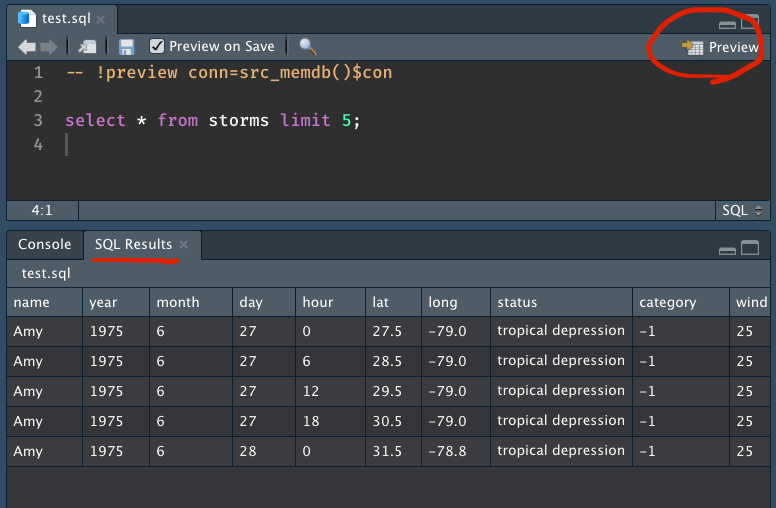
\includegraphics[width=1\linewidth]{./images/Bab3/sql-file-preview} 

}

\caption{Previewing `.sql` in R}\label{fig:unnamed-chunk-55}
\end{figure}

\hypertarget{sql-chunks-in-rmarkdown}{%
\section{SQL chunks in RMarkdown}\label{sql-chunks-in-rmarkdown}}

I generally prefer to show RMarkdown output in the console 1 (and it looks like I'm not the only one). This means that when I run code in an .Rmd file, it feels more or less the same as when I run an .R file: the plots show up in the plots pane, code is run in the console, and so on. While you can use SQL chunks with this setting, there is NO chunk preview option. You must trust your queries and knit the file to make sure everything runs. You get the syntax highlighting razzle-dazzle but alas-- no preview.

It is in this very specific case where inline mode wins big time. SQL previews magically become an option, allowing you to interact with your beautifully colored SQL code.

\hypertarget{database-normalization-in-sql}{%
\chapter{Database Normalization in SQL}\label{database-normalization-in-sql}}

Normalization is a database design technique that reduces data redundancy and eliminates undesirable characteristics like Insertion, Update and Deletion Anomalies. Normalization rules divides larger tables into smaller tables and links them using relationships. The purpose of Normalisation in SQL is to eliminate redundant (repetitive) data and ensure data is stored logically.

The inventor of the relational model Edgar Codd proposed the theory of normalization of data with the introduction of the First Normal Form, and he continued to extend theory with Second and Third Normal Form. Later he joined Raymond F. Boyce to develop the theory of Boyce-Codd Normal Form.

Here is a list of Normal Forms in SQL:

\begin{itemize}
\tightlist
\item
  1NF (First Normal Form)
\item
  2NF (Second Normal Form)
\item
  3NF (Third Normal Form)
\item
  BCNF (Boyce-Codd Normal Form)
\item
  4NF (Fourth Normal Form)
\item
  5NF (Fifth Normal Form)
\item
  6NF (Sixth Normal Form)
\end{itemize}

The Theory of Data Normalization in MySQL server is still being developed further. For example, there are discussions even on 6th Normal Form. However, in most practical applications, normalization achieves its best in 3rd Normal Form.

\hypertarget{the-process-of-normalization}{%
\section{The Process of Normalization}\label{the-process-of-normalization}}

The process of normalization involves breaking down a large table into smaller, related tables and defining relationships between them. This helps in achieving the following benefits:

\begin{itemize}
\tightlist
\item
  \textbf{Elimination of Data Redundancy:} Redundant data can lead to inconsistencies and increased storage requirements. Normalization ensures that each piece of data is stored in only one place, reducing redundancy and promoting consistency.
\item
  \textbf{Data Integrity:} Normalization minimizes the chances of inconsistencies and anomalies that may occur when data is duplicated or updated in one place but not in another.
\item
  \textbf{Efficient Data Updates:} Since data is stored in smaller, more specific tables, updates are more efficient and require fewer changes.
\item
  \textbf{Simpler Queries:} Normalized data allows for more straightforward and efficient querying due to the structured relationships between tables.
\end{itemize}

The process of database normalization is typically divided into several ``normal forms'' (often referred to as 1NF, 2NF, 3NF, BCNF, etc.), each with its own set of rules and requirements. These normal forms build on each other, with higher normal forms addressing more complex issues of redundancy and dependency. Here's a brief overview of some common normal forms:

\begin{enumerate}
\def\labelenumi{\arabic{enumi}.}
\tightlist
\item
  \textbf{First Normal Form (1NF):}
\end{enumerate}

\begin{itemize}
\tightlist
\item
  Eliminate duplicate columns.
\item
  Create separate tables for related data.
\item
  Define a primary key for each table.
\end{itemize}

\begin{enumerate}
\def\labelenumi{\arabic{enumi}.}
\setcounter{enumi}{1}
\tightlist
\item
  \textbf{Second Normal Form (2NF):}
\end{enumerate}

\begin{itemize}
\tightlist
\item
  Meet 1NF requirements.
\item
  Remove partial dependencies (attributes dependent on only part of the primary key) by creating
\item
  separate tables.
\end{itemize}

\begin{enumerate}
\def\labelenumi{\arabic{enumi}.}
\setcounter{enumi}{2}
\tightlist
\item
  \textbf{Third Normal Form (3NF):}
\end{enumerate}

\begin{itemize}
\tightlist
\item
  Meet 2NF requirements.
\item
  Remove transitive dependencies (attributes dependent on non-key attributes) by creating separate tables.
\end{itemize}

\begin{enumerate}
\def\labelenumi{\arabic{enumi}.}
\setcounter{enumi}{3}
\tightlist
\item
  \textbf{Boyce-Codd Normal Form (BCNF):}
\end{enumerate}

\begin{itemize}
\tightlist
\item
  Meet 3NF requirements.
\item
  Remove overlapping candidate keys by creating separate tables.
\end{itemize}

Higher normal forms exist beyond these, such as \textbf{Fourth Normal Form (4NF)} and \textbf{Fifth Normal Form (5NF)}, but they are less commonly encountered and may be more relevant in specific cases of complex data modeling. While normalization offers significant benefits, it's important to strike a balance between normalization and performance. Over-normalization can lead to complex query logic and decreased query performance. Therefore, designing a database often involves considering the nature of the data and the queries that will be performed on it.

\hypertarget{simple-database-normalization}{%
\section{Simple Database Normalization}\label{simple-database-normalization}}

Let's go through a simple example of database normalization using a hypothetical scenario of an online bookstore. We'll start with an unnormalized table and then progressively normalize it through different normal forms.

Scenario: Consider an unnormalized table that stores information about books, authors, and their publishers.

\textbf{Unnormalized Table (1NF):}

\begin{longtable}[]{@{}
  >{\raggedright\arraybackslash}p{(\columnwidth - 10\tabcolsep) * \real{0.1233}}
  >{\raggedright\arraybackslash}p{(\columnwidth - 10\tabcolsep) * \real{0.2329}}
  >{\raggedright\arraybackslash}p{(\columnwidth - 10\tabcolsep) * \real{0.1918}}
  >{\raggedright\arraybackslash}p{(\columnwidth - 10\tabcolsep) * \real{0.1918}}
  >{\raggedright\arraybackslash}p{(\columnwidth - 10\tabcolsep) * \real{0.1781}}
  >{\raggedright\arraybackslash}p{(\columnwidth - 10\tabcolsep) * \real{0.0822}}@{}}
\toprule\noalign{}
\begin{minipage}[b]{\linewidth}\raggedright
Book ID
\end{minipage} & \begin{minipage}[b]{\linewidth}\raggedright
Title
\end{minipage} & \begin{minipage}[b]{\linewidth}\raggedright
Author
\end{minipage} & \begin{minipage}[b]{\linewidth}\raggedright
Author Birth
\end{minipage} & \begin{minipage}[b]{\linewidth}\raggedright
Publisher
\end{minipage} & \begin{minipage}[b]{\linewidth}\raggedright
Year
\end{minipage} \\
\midrule\noalign{}
\endhead
\bottomrule\noalign{}
\endlastfoot
1 & Algorithm & John Smith & 1980-05-15 & ABC Pub & 2000 \\
2 & Data Science & Jane Doe & 1975-10-20 & XYZ Books & 2015 \\
3 & Database System & John Smith & 1980-05-15 & ABC Pub & 2012 \\
\end{longtable}

In this unnormalized table, we have duplicate author and publisher information, leading to redundancy. John Smith's information is repeated, and if any of his details change, we need to update multiple rows.

\textbf{First Normal Form (1NF):}

To achieve 1NF, we break the table into smaller tables and remove duplicate data. We create separate tables for authors and publishers.

Authors Table:

\begin{longtable}[]{@{}lll@{}}
\toprule\noalign{}
Author ID & Author & Author Birth \\
\midrule\noalign{}
\endhead
\bottomrule\noalign{}
\endlastfoot
1 & John Smith & 1980-05-15 \\
2 & Jane Doe & 1975-10-20 \\
\end{longtable}

Publishers Table:

\begin{longtable}[]{@{}ll@{}}
\toprule\noalign{}
Publisher ID & Publisher \\
\midrule\noalign{}
\endhead
\bottomrule\noalign{}
\endlastfoot
1 & ABC Pub \\
2 & XYZ Books \\
\end{longtable}

Books Table (1NF):

\begin{longtable}[]{@{}lllll@{}}
\toprule\noalign{}
Book ID & Title & Author ID & Publisher ID & Year \\
\midrule\noalign{}
\endhead
\bottomrule\noalign{}
\endlastfoot
1 & Algorithm & 1 & 1 & 2000 \\
2 & Data Science & 2 & 2 & 2015 \\
3 & Database System & 1 & 1 & 2012 \\
\end{longtable}

We've eliminated redundancy by referencing author and publisher IDs in the books table.

\textbf{Second Normal Form (2NF):}

To achieve 2NF, we identify partial dependencies and create a separate table for author information.

Authors Table (2NF):

\begin{longtable}[]{@{}lll@{}}
\toprule\noalign{}
Author ID & Author & Author Birth \\
\midrule\noalign{}
\endhead
\bottomrule\noalign{}
\endlastfoot
1 & John Smith & 1980-05-15 \\
2 & Jane Doe & 1975-10-20 \\
\end{longtable}

Books Table (2NF):

\begin{longtable}[]{@{}lllll@{}}
\toprule\noalign{}
Book ID & Title & Author ID & Publisher ID & Year \\
\midrule\noalign{}
\endhead
\bottomrule\noalign{}
\endlastfoot
1 & Algorithm & 1 & 1 & 2000 \\
2 & Data Science & 2 & 2 & 2015 \\
3 & Database System & 1 & 1 & 2012 \\
\end{longtable}

No changes are required in the Books table for 2NF since there were no partial dependencies.

\textbf{Third Normal Form (3NF):}

To achieve 3NF, we identify transitive dependencies and create a separate table for publisher information.

Publishers Table (3NF):

\begin{longtable}[]{@{}ll@{}}
\toprule\noalign{}
Publisher ID & Publisher \\
\midrule\noalign{}
\endhead
\bottomrule\noalign{}
\endlastfoot
1 & ABC Pub \\
2 & XYZ Books \\
\end{longtable}

Books Table (3NF):

\begin{longtable}[]{@{}lllll@{}}
\toprule\noalign{}
Book ID & Title & Author ID & Publisher ID & Year \\
\midrule\noalign{}
\endhead
\bottomrule\noalign{}
\endlastfoot
1 & Algorithm & 1 & 1 & 2000 \\
2 & Data Science & 2 & 2 & 2015 \\
3 & Database System & 1 & 1 & 2012 \\
\end{longtable}

No changes are required in the Books table for 3NF since there were no transitive dependencies. The result is a normalized database structure that eliminates redundancy and ensures data integrity.

Please note that the above example is simplified for demonstration purposes. In real-world scenarios, databases can have more complex structures and relationships, which may require deeper levels of normalization to achieve higher normal forms like BCNF or 4NF.

\hypertarget{your-job-1}{%
\section{Your Job}\label{your-job-1}}

Consider a hypothetical database for an online bookstore. We'll start with a denormalized table and then go through the normalization process step by step.

Suppose we have a single table called Books with the following columns:

\begin{table}

\caption{\label{tab:unnamed-chunk-57}First Normal Form (1NF)}
\centering
\begin{tabular}[t]{l|l|l|l|l|l}
\hline
BookID & Title & Author & Genre & Publisher & PublicationYear\\
\hline
1 & Book A & Author X & Fiction & dsciencelabs & 2021\\
\hline
2 & Book B & Author Y & Mystery & Matana & 2022\\
\hline
3 & Book B & Author X & Romance & dsciencelabs & 2023\\
\hline
\end{tabular}
\end{table}

Your job is the following statements:

\begin{enumerate}
\def\labelenumi{\arabic{enumi}.}
\tightlist
\item
  Display Database Normalization Process
\item
  Create Database to your PC After Normalization Process using R and SQL
\end{enumerate}

\hypertarget{join-table-in-sql}{%
\chapter{Join Table in SQL}\label{join-table-in-sql}}

A SQL join is a Structured Query Language (SQL) instruction to combine data from two sets of data (i.e.~two tables). Before we dive into the details of a SQL join, let's briefly discuss what SQL is, and why someone would want to perform a SQL join.

SQL is a special-purpose programming language designed for managing information in a relational database management system (RDBMS). The word relational here is key; it specifies that the database management system is organized in such a way that there are clear relations defined between different sets of data. Typically, you need to extract, transform, and load data into your RDBMS before you're able to manage it using SQL, which you can accomplish by using a tool like Stitch.

\begin{center}\rule{0.5\linewidth}{0.5pt}\end{center}

\hypertarget{relational-database}{%
\section{Relational Database}\label{relational-database}}

Imagine you're running a store and would like to record information about your customers and their orders. By using a relational database, you can save this information as two tables that represent two distinct entities: customers and orders .

\hypertarget{table-customers}{%
\subsection{Table Customers}\label{table-customers}}

\begin{Shaded}
\begin{Highlighting}[]
\FunctionTok{library}\NormalTok{(DT)}
\NormalTok{costomers}\OtherTok{\textless{}{-}}\FunctionTok{read.csv}\NormalTok{(}\StringTok{"data/customers.csv"}\NormalTok{)}
\FunctionTok{datatable}\NormalTok{(}\FunctionTok{head}\NormalTok{(costomers, }\DecValTok{5}\NormalTok{), }
          \AttributeTok{caption =}\NormalTok{ htmltools}\SpecialCharTok{::}\NormalTok{tags}\SpecialCharTok{$}\FunctionTok{caption}\NormalTok{(}
            \AttributeTok{style =} \StringTok{\textquotesingle{}caption{-}side: bottom; text{-}align: center;\textquotesingle{}}\NormalTok{, }
\NormalTok{            htmltools}\SpecialCharTok{::}\FunctionTok{em}\NormalTok{(}\StringTok{\textquotesingle{}Table 1: customers.\textquotesingle{}}\NormalTok{)),}
          \AttributeTok{options =} \FunctionTok{list}\NormalTok{(}\AttributeTok{dom =} \StringTok{\textquotesingle{}t\textquotesingle{}}\NormalTok{))}
\end{Highlighting}
\end{Shaded}

Table 1, informs about each customer is stored in its own row, with columns specifying different bits of information, including their first name, last name, and email address. Additionally, we associate a unique customer number, or primary key, with each customer record.

\hypertarget{table-orders}{%
\subsection{Table Orders}\label{table-orders}}

\begin{Shaded}
\begin{Highlighting}[]
\NormalTok{orders}\OtherTok{\textless{}{-}}\FunctionTok{read.csv}\NormalTok{(}\StringTok{"data/orders.csv"}\NormalTok{)}
\FunctionTok{datatable}\NormalTok{(}\FunctionTok{head}\NormalTok{(orders,}\DecValTok{5}\NormalTok{), }
          \AttributeTok{caption =}\NormalTok{ htmltools}\SpecialCharTok{::}\NormalTok{tags}\SpecialCharTok{$}\FunctionTok{caption}\NormalTok{(}
            \AttributeTok{style =} \StringTok{\textquotesingle{}caption{-}side: bottom; text{-}align: center;\textquotesingle{}}\NormalTok{, }
\NormalTok{            htmltools}\SpecialCharTok{::}\FunctionTok{em}\NormalTok{(}\StringTok{\textquotesingle{}Table 2: orders.\textquotesingle{}}\NormalTok{)),}
          \AttributeTok{options =} \FunctionTok{list}\NormalTok{(}\AttributeTok{dom =} \StringTok{\textquotesingle{}t\textquotesingle{}}\NormalTok{))}
\end{Highlighting}
\end{Shaded}

Again, Table 2 are contains information about a specific order. Each order has its own unique identification key \texttt{order\_id} for this table -- assigned to it as well.

\hypertarget{relational-model}{%
\section{Relational Model}\label{relational-model}}

You've probably noticed that these two examples share similar information. You can see these simple relations diagrammed below:

\begin{figure}

{\centering 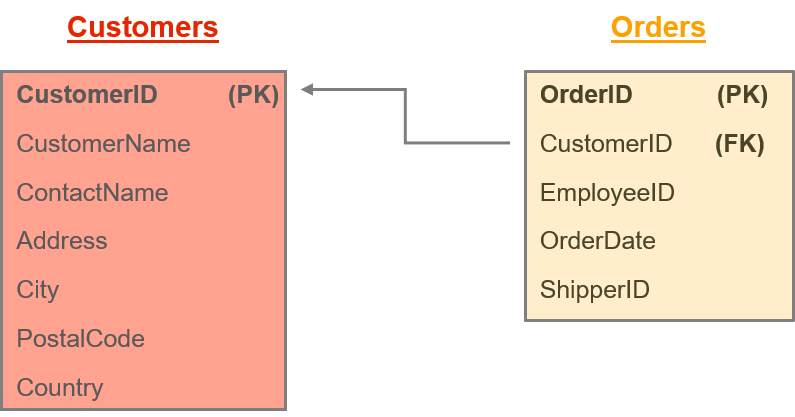
\includegraphics[width=1\linewidth]{./images/Bab5/relational} 

}

\caption{Relational Table}\label{fig:relational}
\end{figure}

Note that the orders table contains two keys: one for the order and one for the customer who placed that order. In scenarios when there are multiple keys in a table, the key that refers to the entity being described in that table is called the primary key \emph{(PK)} and other key is called a foreign key \emph{(FK)}.

In our example, \texttt{order\_id} is a primary key in the orders table, while \texttt{customer\_id} is both a primary key in the customers table and a foreign key in the orders table. Primary and foreign keys are essential to describing relations between the tables, and in performing SQL joins.

\begin{center}\rule{0.5\linewidth}{0.5pt}\end{center}

\hypertarget{factory-database}{%
\section{Factory Database}\label{factory-database}}

To make you more convenient about all the data tables that we will use in this section. Here, I summarize the following SQL relational for database \texttt{factory\_db}:

\begin{figure}

{\centering 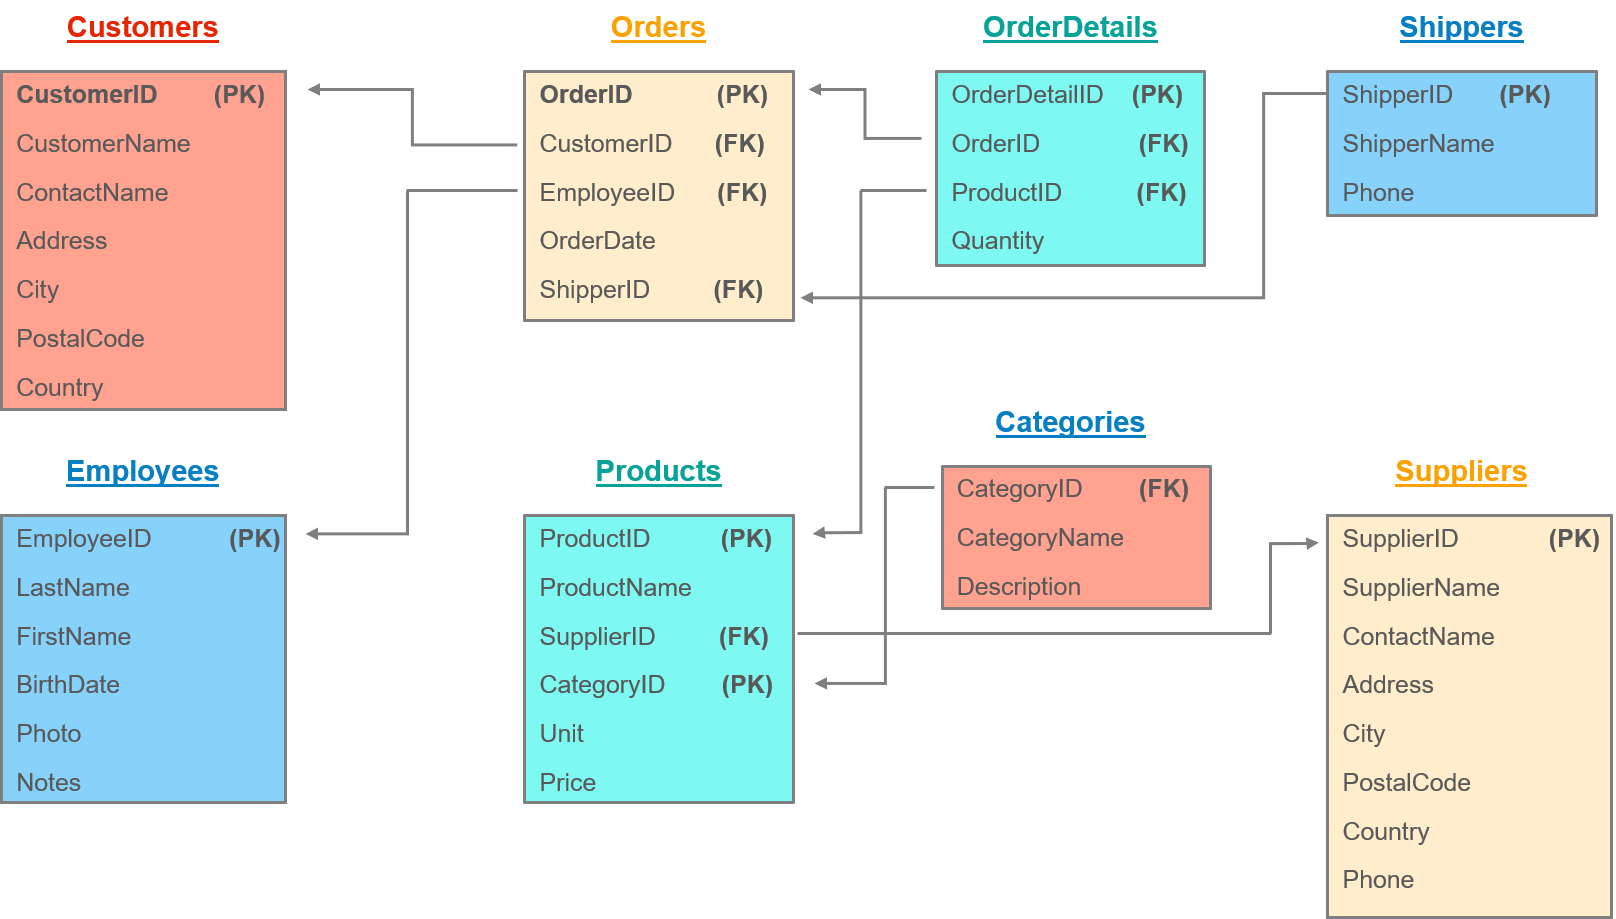
\includegraphics[width=1\linewidth]{./images/Bab5/fullrelational} 

}

\caption{Relational Table of Factory Database}\label{fig:fullrelational}
\end{figure}

\emph{Note:} Don't forget to consider the data structure of your database (all table)

\begin{center}\rule{0.5\linewidth}{0.5pt}\end{center}

\hypertarget{basic-sql-join-types}{%
\section{Basic SQL Join Types}\label{basic-sql-join-types}}

There are four basic types of SQL joins: inner, left, right, and full. The easiest and most intuitive way to explain the difference between these four types is by using a Venn diagram, which shows all possible logical relations between data sets.

Again, it's important to stress that before you can begin using any join type, you'll need to extract the data and load it into an RDBMS like Amazon Redshift, where you can query tables from multiple sources. You build that process manually, or you can use an ETL service like Stitch, which automates that process for you.

\begin{figure}

{\centering 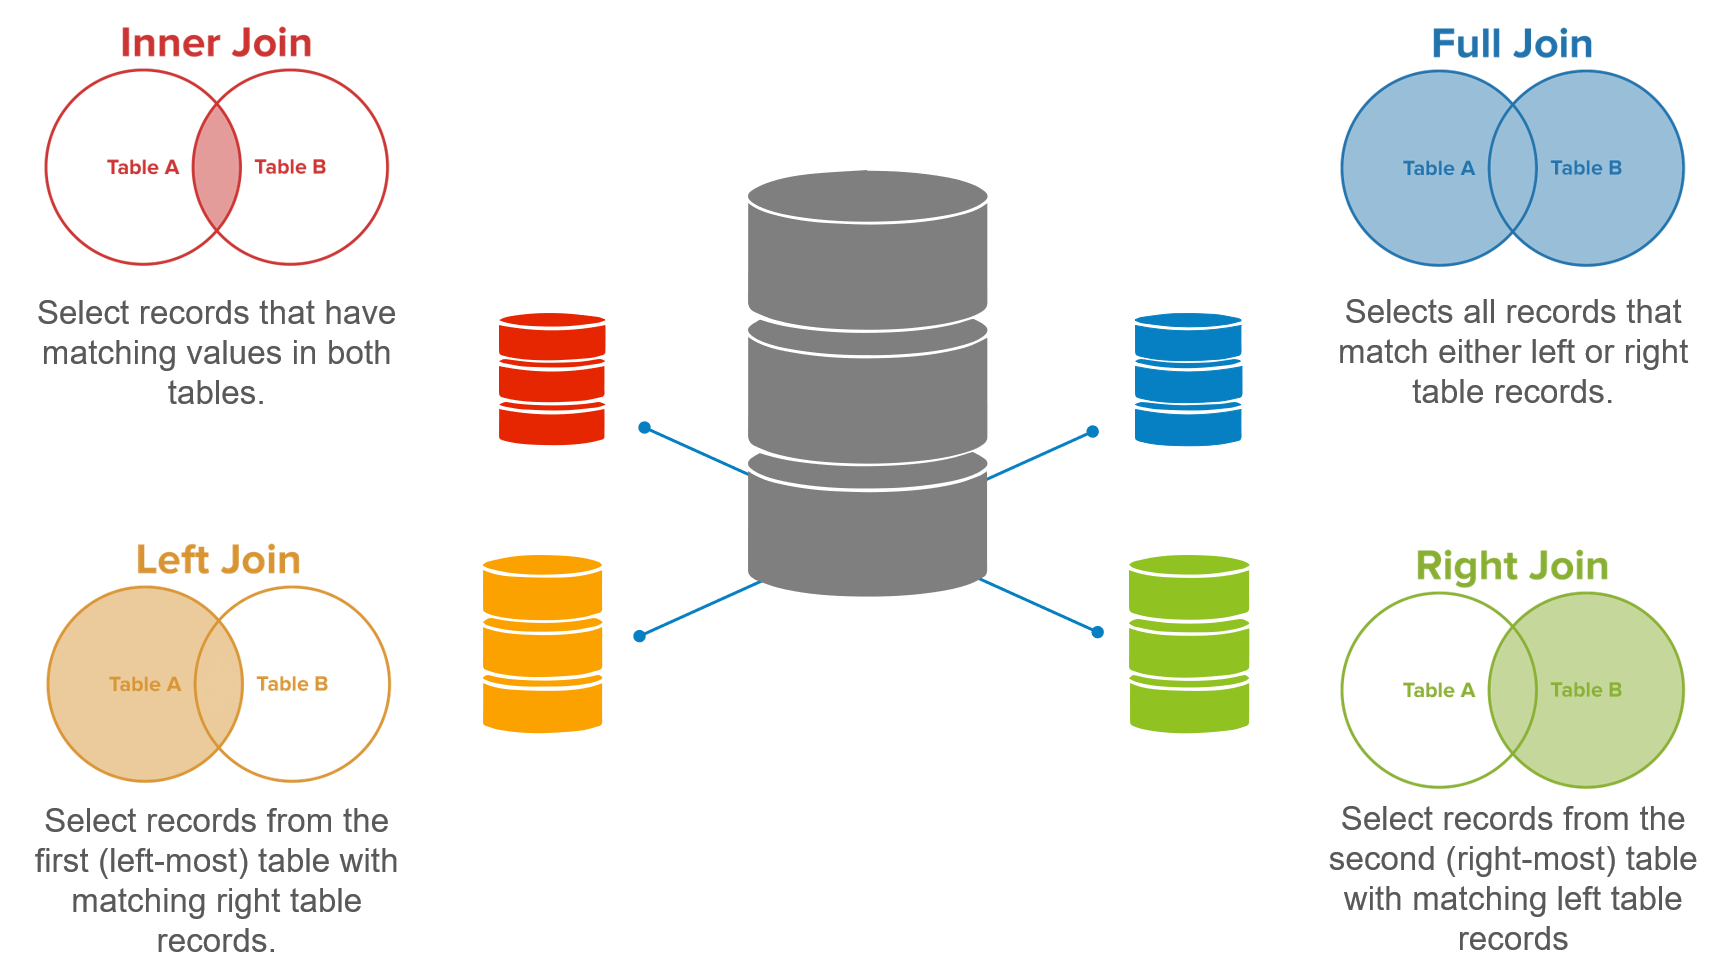
\includegraphics[width=1\linewidth]{./images/Bab5/jointable} 

}

\caption{Basic Join Table}\label{fig:jointable}
\end{figure}

\hypertarget{connect-to-mysql}{%
\section{Connect to MySQL}\label{connect-to-mysql}}

Reading data from \texttt{MySQL} into R workspace, it requires two R libraries, \texttt{RMySQL} and \texttt{DBI}. The connection data should not be embedded in analysis code. Separate the connection code in another script. The script should set up the connection and save it into the workspace.

The saved connection is accessible by its name in the analysis code. In the dbConnect function, you need to replace dbname, username, pwd, dbserver and port with the actual values of your remote database.

\begin{Shaded}
\begin{Highlighting}[]
\CommentTok{\# set up the connection and save it into the workspace}
\CommentTok{\#\textasciitilde{}\textasciitilde{}\textasciitilde{}\textasciitilde{}\textasciitilde{}\textasciitilde{}\textasciitilde{}\textasciitilde{}\textasciitilde{}\textasciitilde{}\textasciitilde{}\textasciitilde{}\textasciitilde{}\textasciitilde{}\textasciitilde{}\textasciitilde{}\textasciitilde{}\textasciitilde{}\textasciitilde{}\textasciitilde{}\textasciitilde{}\textasciitilde{}\textasciitilde{}\textasciitilde{}\textasciitilde{}\textasciitilde{}\textasciitilde{}\textasciitilde{}\textasciitilde{}\textasciitilde{}\textasciitilde{}\textasciitilde{}\textasciitilde{}\textasciitilde{}\textasciitilde{}\textasciitilde{}\textasciitilde{}\textasciitilde{}\textasciitilde{}\textasciitilde{}\textasciitilde{}\textasciitilde{}\textasciitilde{}\textasciitilde{}\textasciitilde{}\textasciitilde{}\textasciitilde{}\textasciitilde{}\textasciitilde{}\textasciitilde{}\textasciitilde{}\textasciitilde{}\textasciitilde{}\textasciitilde{}\textasciitilde{}\textasciitilde{}\textasciitilde{}\textasciitilde{}\textasciitilde{}\textasciitilde{}\textasciitilde{}\textasciitilde{}\textasciitilde{}\textasciitilde{}\textasciitilde{}\textasciitilde{}\textasciitilde{}\textasciitilde{}\textasciitilde{}\textasciitilde{}\textasciitilde{}\textasciitilde{}\textasciitilde{}\textasciitilde{}\textasciitilde{}\textasciitilde{}\textasciitilde{}\textasciitilde{}\textasciitilde{}}
\FunctionTok{library}\NormalTok{(RMySQL)}
\FunctionTok{library}\NormalTok{(DBI)}
\NormalTok{bakti }\OtherTok{\textless{}{-}} \FunctionTok{dbConnect}\NormalTok{(RMySQL}\SpecialCharTok{::}\FunctionTok{MySQL}\NormalTok{(),}
                  \AttributeTok{dbname=}\StringTok{\textquotesingle{}factory\_db\textquotesingle{}}\NormalTok{,}
                  \AttributeTok{username=}\StringTok{\textquotesingle{}root\textquotesingle{}}\NormalTok{,}
                  \AttributeTok{password=}\StringTok{\textquotesingle{}\textquotesingle{}}\NormalTok{, }
                  \AttributeTok{host=}\StringTok{\textquotesingle{}localhost\textquotesingle{}}\NormalTok{,}
                  \AttributeTok{port=}\DecValTok{3306}\NormalTok{)}
\NormalTok{knitr}\SpecialCharTok{::}\NormalTok{opts\_chunk}\SpecialCharTok{$}\FunctionTok{set}\NormalTok{(}\AttributeTok{connection =} \StringTok{"bakti"}\NormalTok{)   }\CommentTok{\# set up the connection }
\end{Highlighting}
\end{Shaded}

After set up the connection and save it into the workspace. Next, we can run SQL in a code chunk of type sql. By setting the connection in the code chuck and adding the option output.var, the resulting table from the SQL is written into a variable in R.

\begin{verbatim}
'''{sql connection=bakti, output.var="report_model_by_make"} 
      Your SQL code Here
'''
\end{verbatim}

\hypertarget{inner-join}{%
\section{Inner Join}\label{inner-join}}

Let's say we wanted to get a list of those customers who placed an order and the details of the order they placed. This would be a perfect fit for an inner join, since an inner join returns records at the intersection of the two tables.

\begin{Shaded}
\begin{Highlighting}[]
\NormalTok{SELECT OrderID, CustomerName}
\NormalTok{  FROM Orders O}
\NormalTok{    INNER JOIN Customers C}
\NormalTok{      ON O.CustomerID }\OtherTok{=}\NormalTok{ C.CustomerID}
\end{Highlighting}
\end{Shaded}

\begin{Shaded}
\begin{Highlighting}[]
\FunctionTok{library}\NormalTok{(DT)}
\FunctionTok{datatable}\NormalTok{(Inner1, }
          \AttributeTok{caption =}\NormalTok{ htmltools}\SpecialCharTok{::}\NormalTok{tags}\SpecialCharTok{$}\FunctionTok{caption}\NormalTok{(}
            \AttributeTok{style =} \StringTok{\textquotesingle{}caption{-}side: bottom; text{-}align: center;\textquotesingle{}}\NormalTok{, }
\NormalTok{            htmltools}\SpecialCharTok{::}\FunctionTok{em}\NormalTok{(}\StringTok{\textquotesingle{}Table 3: SQL Inner Join Two Tables.\textquotesingle{}}\NormalTok{)))}
\end{Highlighting}
\end{Shaded}

The following SQL statement selects all orders with customer and shipper information:

\begin{Shaded}
\begin{Highlighting}[]
\NormalTok{SELECT }\SpecialCharTok{*} 
  \FunctionTok{FROM}\NormalTok{ ((Orders O}
\NormalTok{    INNER JOIN Customers C}
\NormalTok{      ON }\AttributeTok{O.CustomerID =}\NormalTok{ C.CustomerID)}
\NormalTok{    INNER JOIN Shippers S }
\NormalTok{      ON }\AttributeTok{O.ShipperID =}\NormalTok{ S.ShipperID)}
\end{Highlighting}
\end{Shaded}

\begin{Shaded}
\begin{Highlighting}[]
\FunctionTok{datatable}\NormalTok{(Inner2, }
          \AttributeTok{caption =}\NormalTok{ htmltools}\SpecialCharTok{::}\NormalTok{tags}\SpecialCharTok{$}\FunctionTok{caption}\NormalTok{(}
            \AttributeTok{style =} \StringTok{\textquotesingle{}caption{-}side: bottom; text{-}align: center;\textquotesingle{}}\NormalTok{, }
\NormalTok{            htmltools}\SpecialCharTok{::}\FunctionTok{em}\NormalTok{(}\StringTok{\textquotesingle{}Table 4: SQL Inner Join Three Tables.\textquotesingle{}}\NormalTok{)),}
          \AttributeTok{extensions =} \StringTok{\textquotesingle{}FixedColumns\textquotesingle{}}\NormalTok{,}
          \AttributeTok{options =} \FunctionTok{list}\NormalTok{(}\AttributeTok{scrollX =} \ConstantTok{TRUE}\NormalTok{, }\AttributeTok{fixedColumns =} \ConstantTok{TRUE}\NormalTok{)}
\NormalTok{          )}
\end{Highlighting}
\end{Shaded}

\hypertarget{left-join}{%
\section{Left Join}\label{left-join}}

If we wanted to simply append information about orders to our customers table, regardless of whether a customer placed an order or not, we would use a left join. A left join returns all records from table A and any matching records from table B. The result is NULL from the right side, if there is no match.

\begin{Shaded}
\begin{Highlighting}[]
\NormalTok{SELECT CustomerName, OrderID}
\NormalTok{  FROM Customers C}
\NormalTok{    LEFT JOIN Orders O}
\NormalTok{      ON C.CustomerID }\OtherTok{=}\NormalTok{ O.CustomerID}
\NormalTok{        ORDER BY C.CustomerName}
\end{Highlighting}
\end{Shaded}

\begin{Shaded}
\begin{Highlighting}[]
\FunctionTok{datatable}\NormalTok{(Left, }
          \AttributeTok{caption =}\NormalTok{ htmltools}\SpecialCharTok{::}\NormalTok{tags}\SpecialCharTok{$}\FunctionTok{caption}\NormalTok{(}
            \AttributeTok{style =} \StringTok{\textquotesingle{}caption{-}side: bottom; text{-}align: center;\textquotesingle{}}\NormalTok{, }
\NormalTok{            htmltools}\SpecialCharTok{::}\FunctionTok{em}\NormalTok{(}\StringTok{\textquotesingle{}Table 5: SQL Left Join Two Tables.\textquotesingle{}}\NormalTok{)))}
\end{Highlighting}
\end{Shaded}

\hypertarget{right-join}{%
\section{Right Join}\label{right-join}}

The following SQL statement will return all employees, and any orders they might have placed. The result is NULL from the left side, when there is no match.

\begin{Shaded}
\begin{Highlighting}[]
\NormalTok{SELECT OrderID, LastName, FirstName}
\NormalTok{  FROM Orders O}
\NormalTok{    RIGHT JOIN Employees E}
\NormalTok{      ON O.EmployeeID }\OtherTok{=}\NormalTok{ E.EmployeeID}
\NormalTok{        ORDER BY O.OrderID}
\end{Highlighting}
\end{Shaded}

\begin{Shaded}
\begin{Highlighting}[]
\FunctionTok{datatable}\NormalTok{(Right, }
          \AttributeTok{caption =}\NormalTok{ htmltools}\SpecialCharTok{::}\NormalTok{tags}\SpecialCharTok{$}\FunctionTok{caption}\NormalTok{(}
            \AttributeTok{style =} \StringTok{\textquotesingle{}caption{-}side: bottom; text{-}align: center;\textquotesingle{}}\NormalTok{, }
\NormalTok{            htmltools}\SpecialCharTok{::}\FunctionTok{em}\NormalTok{(}\StringTok{\textquotesingle{}Table 6: SQL Right Join Two Tables.\textquotesingle{}}\NormalTok{)))}
\end{Highlighting}
\end{Shaded}

\hypertarget{full-join}{%
\section{Full Join}\label{full-join}}

The FULL OUTER JOIN keyword returns all records when there is a match in left (table1) or right (table2) table records. FULL OUTER JOIN, FULL JOIN, and JOIN (MariaDB) are the same. The following SQL statement selects all customers, and all orders:

\begin{Shaded}
\begin{Highlighting}[]
\NormalTok{SELECT CustomerName, OrderID}
\NormalTok{  FROM Customers C}
\NormalTok{    JOIN Orders O}
\NormalTok{      ON C.CustomerID}\OtherTok{=}\NormalTok{O.CustomerID}
\NormalTok{        ORDER BY C.CustomerName}
\end{Highlighting}
\end{Shaded}

\begin{Shaded}
\begin{Highlighting}[]
\FunctionTok{datatable}\NormalTok{(Full, }
          \AttributeTok{caption =}\NormalTok{ htmltools}\SpecialCharTok{::}\NormalTok{tags}\SpecialCharTok{$}\FunctionTok{caption}\NormalTok{(}
            \AttributeTok{style =} \StringTok{\textquotesingle{}caption{-}side: bottom; text{-}align: center;\textquotesingle{}}\NormalTok{, }
\NormalTok{            htmltools}\SpecialCharTok{::}\FunctionTok{em}\NormalTok{(}\StringTok{\textquotesingle{}Table 7: SQL Full Join Two Tables.\textquotesingle{}}\NormalTok{)))}
\end{Highlighting}
\end{Shaded}

\hypertarget{self-join}{%
\section{Self JOIN}\label{self-join}}

A self JOIN is a regular join, but the table is joined with itself. The following SQL statement matches customers that are from the same city:

\begin{Shaded}
\begin{Highlighting}[]
\NormalTok{SELECT A.CustomerName AS CustomerName1, }
\NormalTok{       B.CustomerName AS CustomerName2, }
\NormalTok{       A.City}
\NormalTok{  FROM Customers A, }
\NormalTok{       Customers B}
\NormalTok{    WHERE A.CustomerID }\SpecialCharTok{\textless{}}\ErrorTok{\textgreater{}}\NormalTok{ B.CustomerID}
\NormalTok{      AND A.City }\OtherTok{=}\NormalTok{ B.City}
\NormalTok{        ORDER BY A.City}
\end{Highlighting}
\end{Shaded}

\begin{Shaded}
\begin{Highlighting}[]
\FunctionTok{datatable}\NormalTok{(Self, }
          \AttributeTok{caption =}\NormalTok{ htmltools}\SpecialCharTok{::}\NormalTok{tags}\SpecialCharTok{$}\FunctionTok{caption}\NormalTok{(}
            \AttributeTok{style =} \StringTok{\textquotesingle{}caption{-}side: bottom; text{-}align: center;\textquotesingle{}}\NormalTok{, }
\NormalTok{            htmltools}\SpecialCharTok{::}\FunctionTok{em}\NormalTok{(}\StringTok{\textquotesingle{}Table 8: SQL Self Join Two Tables.\textquotesingle{}}\NormalTok{)))}
\end{Highlighting}
\end{Shaded}

After finishing the work with the database, close the connection.

\begin{Shaded}
\begin{Highlighting}[]
\NormalTok{DBI}\SpecialCharTok{::}\FunctionTok{dbDisconnect}\NormalTok{(bakti)}
\end{Highlighting}
\end{Shaded}

\hypertarget{your-job-2}{%
\section{Your Job}\label{your-job-2}}

\begin{enumerate}
\def\labelenumi{\arabic{enumi}.}
\item
  Apply Left join and Right join to returns all records from table Orders and any matching records from table Suppliers.
\item
  Choose the correct JOIN clause to select all records from the two tables (Orders and Suppliers) where there is a match in both tables.
\item
  Choose the correct JOIN clause to select all the records from the Suppliers table plus all the matches in the Orders table.
\end{enumerate}

\hypertarget{referensi}{%
\chapter{Referensi}\label{referensi}}

  \bibliography{book.bib,packages.bib}

\end{document}
